
% 定义 release 变量就表示发布(编译所有的文件)
\providecommand{\release}{Release}

% 增加review命令表示盲审的论文(除去个人和导师信息)
%\providecommand{\review}{Review}


% /data2/whd/win10/doc/thesis/模板/latex/hnuthesis_master_v4.0
% !Mode:: "TeX:UTF-8"
\def\usewhat{dvipdfmx}                               % 定义编译方式 dvipdfmx 或者 pdflatex ,默认为 dvipdfmx
% 方式编译,如果需要修改,只需改变花括号中的内容即可。
%\setlength{\baselineskip}{20pt}
%\setlength{\headheight}{25pt}
\documentclass[a4paper,12pt,openany,twoside]{book}


% setup/package:存放论文所使用的宏包和全文格式的定义。
% 如果论文超过60页 可以使用twoside 双面打印
% !Mode:: "TeX:UTF-8"
%  Authors: 杜家宜   Jiayi Du: Max_dujiayi@gmail.com     湖南大学2010级计算机科学与技术专业博士生

%%%%%%%%%% Package %%%%%%%%%%%%
\usepackage{supertabular}
\usepackage{threeparttable}
\usepackage{mathtools}
\usepackage{bigstrut}
\usepackage[chapter]{algorithm}
\usepackage{algorithmic}
\usepackage{rotating}
%\usepackage[ruled, linesnumbered]{algorithm2e}
\usepackage{graphicx}                       % 支持插图处理
\usepackage{geometry}
\geometry{left=2.5cm,right=2.5cm,top=2.2cm,bottom=2.2cm,footskip=1.1cm,headsep=0.7cm,head=0.4cm}
%\usepackage[a4paper,text={158true mm,253true mm},top=22true mm,left=25true mm,head=5true mm,foot=11true mm]{geometry} %设置边距 郑伟华 将text={160true mm,253true mm} 改为 text={158true mm,253true mm}

\usepackage{titlesec}                       % 控制标题的宏包
\usepackage{titletoc}                       % 控制目录的宏包
\usepackage{fancyhdr}                       % fancyhdr宏包 支持页眉和页脚的相关定义
\usepackage[UTF8]{ctex}                     % 支持中文显示
\usepackage{cite}
\usepackage{color}                          % 支持彩色
\usepackage{amsmath}                        % AMSLaTeX宏包 用来排出更加漂亮的公式
\usepackage{amssymb}                        % 数学符号生成命令
\usepackage[below]{placeins}                %允许上一个section的浮动图形出现在下一个section的开始部分,还提供\FloatBarrier命令,使所有未处理的浮动图形立即被处理
\usepackage{flafter}                        % 使得所有浮动体不能被放置在其浮动环境之前,以免浮动体在引述它的文本之前出现.
\usepackage{multirow}                       % 使用Multirow宏包,使得表格可以合并多个row格
\usepackage{booktabs}                       % 表格,横的粗线;\specialrule{1pt}{0pt}{0pt}
\usepackage{longtable}                      % 支持跨页的表格。
\usepackage{tabularx}                       % 自动设置表格的列宽
\usepackage{setspace}
\usepackage{subfigure}                      % 支持子图 %centerlast 设置最后一行是否居中
\usepackage[subfigure]{ccaption}            % 支持子图的中文标题
\usepackage[sort&compress,numbers]{natbib}  % 支持引用缩写的宏包
\usepackage{enumitem}                       % 使用enumitem宏包,改变列表项的格式
\usepackage{calc}                           % 长度可以用+ - * / 进行计算
\usepackage{txfonts}                        % 字体宏包
\usepackage{bm}                             % 处理数学公式中的黑斜体的宏包
\usepackage[amsmath,thmmarks,hyperref]{ntheorem}  % 定理类环境宏包,其中 amsmath 选项用来兼容 AMS LaTeX 的宏包
\usepackage{CJKnumb}                        % 提供将阿拉伯数字转换成中文数字的命令
\usepackage{indentfirst}                    % 首行缩进宏包
\usepackage{CJKutf8}                        % 用在UTF8编码环境下,它可以自动调用CJK,同时针对UTF8编码作了设置。
\usepackage{CJK}
\usepackage{fancyhdr}
\usepackage{lastpage}
\usepackage{layout}
\usepackage{graphicx}
\usepackage{subfigure}
\usepackage[titles,subfigure]{tocloft}                       %控制生成的表格和图片的目录格式
%\usepackage{hyperref}
%\usepackage{hypbmsec}                      % 用来控制书签中标题显示内容

% 适应Ubuntu编译
\usepackage[UTF8]{ctex}  % 设置为中文编译(否则为日语)
\usepackage{tikz}
\usetikzlibrary{chains}
\usepackage{smartdiagram}

% 跨tex文件进行引用,在引用的源文件中加入:\externaldocument{chap3}
\usepackage{xr}

% 引入条件编译(调试文档)
\usepackage{ifthen}

% 判断在哪个平台上进行编译:\ifwindows, \iflinux, \ifmacosx 和 \ifcygwin
\usepackage{ifplatform}

%如果您的pdf制作中文书签有乱码使用如下命令,就可以解决了
\usepackage[unicode,               % pdflatex, pdftex 这里决定运行文件的方式不同
            pdfstartview=FitH,
            %CJKbookmarks=true,
            bookmarksnumbered=true,
            bookmarksopen=true,
            colorlinks=true,
            pdfborder={0 0 1},
            citecolor=black,
            linkcolor=black,
            anchorcolor=black,
            urlcolor=black,
            breaklinks=true
            ]{hyperref}

\hypersetup{hidelinks}
                      % 定义本文所使用宏包(\input仅仅把另一个文件导入到主tex文件中)
\graphicspath{{figures/}}                  % 定义所有的.eps文件在figures子目录下


\begin{document}                           % 开始全文
%	\begin{CJK*}{UTF8}{song}                   % 开始中文字体使用(Ubuntu中编译有问题)
		% setup/package: 存放论文所使用全文格式的定义。
		% !Mode:: "TeX:UTF-8"
%  Authors: 杜家宜   Jiayi Du: Max_dujiayi@gmail.com     湖南大学2010级计算机科学与技术专业博士生

%%%%%%%%%% Fonts Definition and Basics %%%%%%%%%%%%%%%%%
\newcommand{\song}{\CJKfamily{song}}    % 宋体
\newcommand{\fs}{\CJKfamily{fs}}        % 仿宋体
\newcommand{\kai}{\CJKfamily{kai}}      % 楷体
\newcommand{\hei}{\CJKfamily{hei}}      % 黑体
\newcommand{\li}{\CJKfamily{li}}        % 隶书
\newcommand{\yihao}{\fontsize{26pt}{26pt}\selectfont}       % 一号, 1.倍行距
\newcommand{\xiaoyi}{\fontsize{24pt}{24pt}\selectfont}      % 小一, 1.倍行距
\newcommand{\erhao}{\fontsize{22pt}{22pt}\selectfont}       % 二号, 1.倍行距
\newcommand{\xiaoer}{\fontsize{18pt}{18pt}\selectfont}      % 小二, 单倍行距
\newcommand{\sanhao}{\fontsize{16pt}{16pt}\selectfont}      % 三号, 1.倍行距
\newcommand{\xiaosan}{\fontsize{15pt}{15pt}\selectfont}     % 小三, 1.倍行距
\newcommand{\sihao}{\fontsize{14pt}{14pt}\selectfont}       % 四号, 1.0倍行距
\newcommand{\xiaosi}{\fontsize{12pt}{12pt}\selectfont}      % 小四, 1.倍行距
\newcommand{\wuhao}{\fontsize{10.5pt}{10.5pt}\selectfont}   % 五号, 单倍行距
\newcommand{\xiaowu}{\fontsize{9pt}{9pt}\selectfont}        % 小五, 单倍行距
\newcommand{\liuhao}{\fontsize{8pt}{8pt}\selectfont}        % 小六, 单倍行距
\setlength{\headheight}{20pt}
%\CJKcaption{gb_452}
%\CJKtilde  % 重新定义了波浪符~的意义
\newcommand\prechaptername{第}
\newcommand\postchaptername{章}

% 调整罗列环境的布局
\setitemize{leftmargin=3em,itemsep=0em,partopsep=0em,parsep=0em,topsep=-0em}
\setenumerate{leftmargin=3em,itemsep=0em,partopsep=0em,parsep=0em,topsep=0em}


%避免宏包 hyperref 和 arydshln 不兼容带来的目录链接失效的问题。
\def\temp{\relax}
\let\temp\addcontentsline
\gdef\addcontentsline{\phantomsection\temp}

% 自定义项目列表标签及格式 \begin{publist} 列表项 \end{publist}
\newcounter{pubctr} %自定义新计数器
\newenvironment{publist}{%%%%%定义新环境
	\begin{list}{[\arabic{pubctr}]} %%标签格式
		{
			\usecounter{pubctr}
			\setlength{\leftmargin}{2em}     % 左边界 \leftmargin =\itemindent + \labelwidth + \labelsep
			\setlength{\itemindent}{0em}     % 标号缩进量
			\setlength{\labelsep}{1em}       % 标号和列表项之间的距离,默认0.5em
			\setlength{\rightmargin}{0em}    % 右边界
			\setlength{\topsep}{0ex}         % 列表到上下文的垂直距离
			\setlength{\parsep}{0ex}         % 段落间距
			\setlength{\itemsep}{0ex}        % 标签间距
			\setlength{\listparindent}{0pt} % 段落缩进量
		}}
		{\end{list}}%%%%%
	
	
	\makeatletter
	\renewcommand\normalsize{
		\@setfontsize\normalsize{12pt}{12pt} % 小四对应12.25pt
		\setlength\abovedisplayskip{4pt}
		\setlength\abovedisplayshortskip{4pt}
		\setlength\belowdisplayskip{\abovedisplayskip}
		\setlength\belowdisplayshortskip{\abovedisplayshortskip}
		\let\@listi\@listI}
	\def\defaultfont{\renewcommand{\baselinestretch}{1.7}\normalsize\selectfont}
	
	% 设置行距和段落间垂直距离
	\setlength{\baselineskip}{20pt}
	\renewcommand{\CJKglue}{\hskip 0.5pt plus \baselineskip} %加大字间距,使每行35个字
	
	
	\makeatother
	
%%%%%%%%%%%%% Contents %%%%%%%%%%%%%%%%%
\renewcommand{\contentsname}{目\qquad 录}
\setcounter{tocdepth}{2}
\titlecontents{chapter}[0em]{\xiaosi\hei}%
{\prechaptername~~\thecontentslabel~~\postchaptername~~~}{} %
{\titlerule*[5pt]{$\cdot$}\xiaosi\contentspage}
\titlecontents{section}[2em]{\xiaosi\song} %
{\thecontentslabel\quad}{} %
{\hspace{.25em}\titlerule*[5pt]{$\cdot$}\xiaosi\contentspage}
\titlecontents{subsection}[4em]{\xiaosi\song} %
{\thecontentslabel\quad}{} %
{\hspace{.25em}\titlerule*[5pt]{$\cdot$}\xiaosi\contentspage}
\renewcommand{\cftdotsep}{1.1}
\renewcommand{\listfigurename}{插图索引}
\setcounter{lofdepth}{1}
%\titlefigures{chapter}[1em]{\xiaosi\hei}%
%             {\prechaptername~~\thecontentslabel~~\postchaptername~~~}{} %
%            {\titlerule*[5pt]{$\cdot$}\xiaosi\contentspage}
\renewcommand{\listtablename}{附表索引}
	
	
%%删除表格和插图因章不同中的空行%%%
\makeatletter
\def\@chapter[#1]#2{\ifnum \c@secnumdepth >\m@ne
	\if@mainmatter
	\refstepcounter{chapter}%
	\typeout{\@chapapp\space\thechapter.}%
	\addcontentsline{toc}{chapter}%
	{\protect\numberline{\thechapter}#1}%
	\else
	\addcontentsline{toc}{chapter}{#1}%
	\fi
	\else
	\addcontentsline{toc}{chapter}{#1}%
	\fi
	\chaptermark{#1}%
	\if@twocolumn
	\@topnewpage[\@makechapterhead{#2}]%
	\else
	\@makechapterhead{#2}%
	\@afterheading
	\fi}
\makeatother
	
	
	%%%%%%%%%% Chapter and Section %%%%%%%%%%%%%%%%%
	\setcounter{secnumdepth}{4}
	\setlength{\parindent}{2em}
	\renewcommand{\chaptername}{\prechaptername\arabic{chapter}\postchaptername}
	\titleformat{\chapter}{\centering\xiaoer\hei}{\chaptername}{1em}{}
	\titlespacing{\chapter}{0pt}{0pt}{18pt}
	\titleformat{\section}{\xiaosan\hei}{\thesection}{1em}{}
	\titlespacing{\section}{0pt}{12pt}{12pt}
	\titleformat{\subsection}{\sihao\hei}{\thesubsection}{0.5em}{}
	\titlespacing{\subsection}{0pt}{6pt}{6pt}
	\titleformat{\subsubsection}{\xiaosi\hei}{\thesubsubsection}{0.5em}{}
	\titlespacing{\subsubsection}{0pt}{6pt}{6pt}

%%%%%%%%%% Table, Figure and Equation %%%%%%%%%%%%%%%%%
\renewcommand{\tablename}{表} % 插表题头
\renewcommand{\figurename}{图} % 插图题头
\renewcommand{\thefigure}{\arabic{chapter}.\arabic{figure}} % 使图编号为 7.1 的格式 %\protect{~}
\renewcommand{\thetable}{\arabic{chapter}.\arabic{table}}%使表编号为 7.1 的格式
\renewcommand{\theequation}{\arabic{chapter}.\arabic{equation}}%使公式编号为 7.1 的格式
\renewcommand{\thesubfigure}{(\alph{subfigure})}%使子图编号为 (a)的格式
\renewcommand{\thesubtable}{(\alph{subtable})} %使子表编号为 (a)的格式
\makeatletter
\renewcommand{\p@subfigure}{\thefigure~} %使子图引用为 7.1 a) 的格式,母图编号和子图编号之间用~ 加一个空格
\makeatother


%% 定制浮动图形和表格标题样式
\makeatletter
\long\def\@makecaption#1#2{%
   \vskip\abovecaptionskip
   \sbox\@tempboxa{\centering\wuhao\hei{#1~~#2} }%
   \ifdim \wd\@tempboxa >\hsize
     \centering\wuhao\hei{#1~~#2} \par
   \else
     \global \@minipagefalse
     \hb@xt@\hsize{\hfil\box\@tempboxa\hfil}%
   \fi
   \vskip\belowcaptionskip}
\makeatother
\captiondelim{~~~~} %用来控制longtable表头分隔符

%%%%%%%%%% Theorem Environment %%%%%%%%%%%%%%%%%
\theoremstyle{plain}
\theorembodyfont{\song\rmfamily}
\theoremheaderfont{\hei\rmfamily}
\newtheorem{theorem}{定理~}[chapter]
\newtheorem{lemma}{引理~}[chapter]
\newtheorem{axiom}{公理~}[chapter]
\newtheorem{proposition}{命题~}[chapter]
\newtheorem{corollary}{推论~}[chapter]
\newtheorem{definition}{定义~}[chapter]
\newtheorem{conjecture}{猜想~}[chapter]
\newtheorem{example}{例~}[chapter]
\newtheorem{remark}{注~}[chapter]
\floatname{algorithm}{算法}%将英文的algorithm改为算法
\renewcommand{\algorithmicrequire}{\textbf{Input:}}
\renewcommand{\algorithmicensure}{\textbf{Output:}}
\newcommand{\tabincell}[2]{\begin{tabular}{@{}#1@{}}#2\end{tabular}}%表格合并
\newenvironment{proof}{\noindent{\hei 证明:}}{\hfill $ \square $ \vskip 4mm}
\theoremsymbol{$\square$}

%%%%%%%%%% Page: number, header and footer  页码%%%%%%%%%%%%%%%%%

%\frontmatter 或 \pagenumbering{roman}
%\mainmatter 或 \pagenumbering{arabic}
% newcommand 是定义一个系统不存在的命令,用户为了方便自己可以定义便于自己阅读和使用的命令
% renewcommand 是重定义一个命令, 我们可以把系统的已有的命令进行重定义
\makeatletter
\renewcommand\frontmatter{\clearpage
  \@mainmatterfalse
  \pagenumbering{Roman}} % 正文前罗马字体编号
\makeatother


%%%%%%%%%% References %%%%%%%%%%%%%%%%%
\renewcommand{\bibname}{参考文献}
% 重定义参考文献样式,来自thu
\makeatletter
\renewenvironment{thebibliography}[1]{%
   \chapter*{\bibname}%
   \xiaosi
   \list{\@biblabel{\@arabic\c@enumiv}}%
        {\renewcommand{\makelabel}[1]{##1\hfill}
         \setlength{\baselineskip}{21pt}
         \settowidth\labelwidth{0.5cm}
         \setlength{\labelsep}{0pt}
         \setlength{\itemindent}{0pt}
         \setlength{\leftmargin}{\labelwidth+\labelsep}
         \addtolength{\itemsep}{-0.7em}
         \usecounter{enumiv}%
         \let\p@enumiv\@empty
         \renewcommand\theenumiv{\@arabic\c@enumiv}}%
    \sloppy\frenchspacing
    \clubpenalty4000%
    \@clubpenalty \clubpenalty
    \widowpenalty4000%
    \interlinepenalty4000%
    \sfcode`\.\@m}
   {\def\@noitemerr
     {\@latex@warning{Empty `thebibliography' environment}}%
    \endlist\frenchspacing}
\makeatother

\addtolength{\bibsep}{5pt} % 增加参考文献间的垂直间距
\setlength{\bibhang}{2em} %每个条目自第二行起缩进的距离

% 参考文献引用作为上标出现
\newcommand{\mycite}[1]{\scalebox{1.3}[1.3]{\raisebox{-0.65ex}{\cite{#1}}}}
%\newcommand{\citenormal}[1]{\cite{#1}}
%\makeatletter
%   \def\@cite#1#2{\textsuperscript{[{#1\if@tempswa , #2\fi}]}}
%\makeatother

%% 引用格式
\bibpunct{[}{]}{,}{s}{}{,}

%%%%%%%%%% Cover %%%%%%%%%%%%%%%%%
% 封面、摘要、版权、致谢格式定义
\makeatletter

%\def\dtitle#1{\def\@dtitle{#1}}\def\@dtitle{}
\def\ctitle#1{\def\@ctitle{#1}}\def\@ctitle{}
\def\etitle#1{\def\@etitle{#1}}\def\@etitle{}
\def\caffil#1{\def\@caffil{#1}}\def\@caffil{}
\def\cmacrosubject#1{\def\@cmacrosubject{#1}}\def\@cmacrosubject{}
\def\cmacrosubjecttitle#1{\def\@cmacrosubjecttitle{#1}}\def\@cmacrosubjecttitle{}
\def\csubject#1{\def\@csubject{#1}}\def\@csubject{}
\def\csubjecttitle#1{\def\@csubjecttitle{#1}}\def\@csubjecttitle{}
\def\cmajor#1{\def\@cmajor{#1}}\def\@cmajor{}
\def\cauthor#1{\def\@cauthor{#1}}\def\@cauthor{}
\def\cauthortitle#1{\def\@cauthortitle{#1}}\def\@cauthortitle{}
\def\csupervisor#1{\def\@csupervisor{#1}}\def\@csupervisor{}
\def\csupervisortitle#1{\def\@csupervisortitle{#1}}\def\@csupervisortitle{}
\def\cdate#1{\def\@cdate{#1}}\def\@cdate{}
\def\untitle#1{\def\@untitle{#1}}\def\@untitle{}
\def\declaretitle#1{\def\@declaretitle{#1}}\def\@declaretitle{}
\def\declarecontent#1{\def\@declarecontent{#1}}\def\@declarecontent{}
\def\authorizationtitle#1{\def\@authorizationtitle{#1}}\def\@authorizationtitle{}
\def\authorizationcontent#1{\def\@authorizationcontent{#1}}\def\@authorizationconent{}
\def\authorizationadd#1{\def\@authorizationadd{#1}}\def\@authorizationadd{}
\def\authorsigncap#1{\def\@authorsigncap{#1}}\def\@authorsigncap{}
\def\supervisorsigncap#1{\def\@supervisorsigncap{#1}}\def\@supervisorsigncap{}
\def\signdatecap#1{\def\@signdatecap{#1}}\def\@signdatecap{}
\long\def\cabstract#1{\long\def\@cabstract{#1}}\long\def\@cabstract{}
\long\def\eabstract#1{\long\def\@eabstract{#1}}\long\def\@eabstract{}
\def\ckeywords#1{\def\@ckeywords{#1}}\def\@ckeywords{}
\def\ekeywords#1{\def\@ekeywords{#1}}\def\@ekeywords{}
\def\cheading#1{\def\@cheading{#1}}\def\@cheading{}
\def\cnumber#1{\def\@cnumber{#1}}\def\@cnumber{}
\def\csecret#1{\def\@csecret{#1}}\def\@csecret{}
\def\chnunumer#1{\def\@chnunumer{#1}}\def\@chnunumer{}
\def\cclassnumber#1{\def\@cclassnumber{#1}}\def\@cclassnumber{}
\def\chnuname#1{\def\@chnuname{#1}}\def\@chnuname{}
\def\cchair#1{\def\@cchair{#1}}\def\@cchair{}
\def\ddate#1{\def\@ddate{#1}}\def\@ddate{}
%英文内封
\def\ename#1{\def\@ename{#1}}\def\@ename{}
\def\cbe#1{\def\@cbe{#1}}\def\@cbe{}
\def\cms#1{\def\@cms{#1}}\def\@cms{}
\def\cdegree#1{\def\@cdegree{#1}}\def\@cdegree{}
\def\cclass#1{\def\@cclass{#1}}\def\@cclass{}
\def\emajor#1{\def\@emajor{#1}}\def\@emajor{}
\def\ehnu#1{\def\@ehnu{#1}}\def\@ehnu{}
\def\esupervisor#1{\def\@esupervisor{#1}}\def\@esupervisor{}
\def\edate#1{\def\@edate{#1}}\def\@edate{}
\def\elevel#1{\def\@elevel{#1}}\def\@elevel{}



\newlength{\@title@width}
\def\@put@covertitle#1{\makebox[\@title@width][s]{#1}}
% 定义封面
\def\makecover{
%\cleardoublepage%
   \phantomsection
    \pdfbookmark[-1]{\@ctitle}{ctitle}

    \begin{titlepage}
    \begin{center}

      \setlength{\@title@width}{3.5cm}
       {
  \begin{tabular}{lcclc}
  	\xiaosi\hei{学校代号}&  \underline{\makebox[\@title@width][c]{\@chnunumer}}&\qquad \qquad \qquad \qquad \qquad & \xiaosi\hei{学\qquad 号}&  \underline{\makebox[\@title@width][c]{\@cnumber}}\\
  	\xiaosi\hei{分~~类~~~号}&  \underline{\makebox[\@title@width][c]{\@cclassnumber}}&\qquad \qquad \qquad \qquad \qquad & \xiaosi\hei{密\qquad 级}&  \underline{\makebox[\@title@width][c]{\@csecret}} \\
  \end{tabular}
   }

 \begin{figure}[h]
  \centering
  
\includegraphics[width=0.3\textwidth]{figures/Hnulogo}
  \end{figure}
      \vspace*{1cm}
      {\hei\erhao \@cheading}

      \vspace*{1cm}


      \begin{center}
      \begin{spacing}{1.5}
      \hei\yihao \@ctitle
      \end{spacing}
      \end{center}

      \vspace{\baselineskip}
      \setlength{\@title@width}{6.5cm}
  {

  \begin{spacing}{2.1}
   \xiaosi\hei{学位申请人姓名} \xiaosi\song\underline{\makebox[\@title@width][l]{\qquad\@cauthor}} \\
   \xiaosi\hei{培~~~~养~~~~~单~~~~~位} \xiaosi\song\underline{\makebox[\@title@width][l]{\qquad\@caffil}} \\
   \xiaosi\hei{导师姓名及职称} \xiaosi\song\underline{\makebox[\@title@width][l]{\qquad\@csupervisor}} \\
   \xiaosi\hei{学~~~~科~~~~~专~~~~~业} \xiaosi\song\underline{\makebox[\@title@width][l]{\qquad\@csubject}} \\
   \xiaosi\hei{研~~~~究~~~~~方~~~~~向} \xiaosi\song\underline{\makebox[\@title@width][l]{\qquad\@cmajor}}\\
   \xiaosi\hei{论~文~提~交~日~~期} \xiaosi\song\underline{\makebox[\@title@width][l]{\qquad\@cdate}} \\
  %\end{tabular}
  \end{spacing}
 }
 \end{center}


\clearpage
\thispagestyle{empty} %去掉页眉页脚

\noindent
\makebox[2.59cm][s]{}{\begin{tabular}{ll}
\xiaosi\hei 学校代号:\xiaosi\song~~\@chnunumer \\
\xiaosi\hei 学\qquad~号:\xiaosi\song~~\@cnumber\\
\xiaosi\hei 密\qquad~级:\xiaosi\song~~\@csecret\\
\end{tabular}
}

%
\vspace{5\baselineskip}

\noindent
\makebox[2.59cm][s]{}{
\xiaoer\song \@chnuname \@cheading
}
\\
\vspace{4\baselineskip}

\begin{spacing}{2}
\hangafter=1\hangindent=2.7cm   %换行后自动缩进
{\noindent
\makebox[2.59cm][s]{} {\hei\erhao\@ctitle}}
\end{spacing}
\vspace{4\baselineskip}

\setlength{\@title@width}{6.5cm}
  {
  \begin{spacing}{2}
  \xiaosi
  \noindent
  \makebox[2.59cm][s]{}{
    \begin{tabular}{lc}
   \underline{\xiaosi\hei学位申请人姓名:\song\makebox[\@title@width][l]{\qquad\qquad\@cauthor}} \\
   \underline{\xiaosi\hei导师姓名及职称:\song\makebox[\@title@width][l]{\qquad\qquad\@csupervisor}} \\
   \underline{\xiaosi\hei培~~~~养~~~~单~~~~位: \song\makebox[\@title@width][l]{\qquad\qquad\@caffil}} \\
   \underline{\xiaosi\hei专~~~~业~~~~名~~~~称: \song\makebox[\@title@width][l]{\qquad\qquad\@csubject}} \\
   \underline{\xiaosi\hei论~文~提~交~日~期:\song\makebox[\@title@width][l]{\qquad\qquad\@cdate}} \\
   \underline{\xiaosi\hei论~文~答~辩~日~期:\song\makebox[\@title@width][l]{\qquad\qquad\@ddate}}\\
   \underline{\xiaosi\hei答辩委员会主席: \song\makebox[\@title@width][l]{\qquad\qquad\@cchair}} \\
  \end{tabular}
   }
   \end{spacing}
    }

\clearpage
\thispagestyle{empty} %去掉页眉页脚

\begin{center}
\qquad\\
 \begin{spacing}{2.5}
 \xiaosan \@etitle

 \end{spacing}



 \begin{spacing}{2}
 \xiaosi
 by\\
 \@ename \\
 \@cbe\\
 \@cms\\
 A~\@cdegree~submitted in partial satisfaction of the\\
 requirements for the degree of\\
 \@cclass\\
 in\\
 \@emajor\\
 in the\\
 Graduate School\\
 of\\
 \@ehnu\\

 \vspace{2\baselineskip}

 Supervisor\\
 Professor \@esupervisor\\
 \@edate
\end{spacing}
\end{center}


\end{titlepage}

%  另起一页: 独创性声明和学位论文版权使用授权书

\pagestyle{fancy}
\fancyhf{}
\fancyfoot[C]{\song\xiaowu ~\thepage~}
\renewcommand{\headrulewidth}{0pt}

    \addcontentsline{toc}{chapter}{学位论文原创性声明和学位论文版权使用授权书}{
    \setcounter{page}{1}
    \qquad\\
    \begin{center}\hei\xiaoer{\@untitle}\end{center}\par
    \begin{center}\hei\xiaoer{\@declaretitle}\end{center}\par
    \song\defaultfont{\@declarecontent}\par
    \vspace*{1cm}
    {\song\xiaosi
    \@authorsigncap \makebox[2.5cm][s]{}
    \@signdatecap \makebox[2cm][s]{} 年 \makebox[1cm][s]{} 月 \makebox[1cm][s]{} 日
    }
    \vspace{0.6\baselineskip}
    \begin{center}\hei\xiaoer{\@authorizationtitle}\end{center}\par
    {
    \vspace{1.2\baselineskip}
    \song\defaultfont{\@authorizationcontent}	
	
	
	\noindent
    \begin{tabular}{ll}
	\song\defaultfont\@authorizationadd\par&\\
    &1、保密\song\xiaoer{$\Box$}\song\xiaosi ,在\underline{\qquad}年解密后适用于本授权书\\
    &2、不保密\song\xiaoer{$\Box$}。\\
    &(请在以上相应方框内打"$\surd$") \\
    \end{tabular}
    }
    \vspace{2\baselineskip}

    {
    \song\xiaosi
      \@authorsigncap \makebox[3.5cm][s]{}  \@signdatecap \makebox[1.5cm][s]{} 年 \makebox[1cm][s]{} 月 \makebox[1cm][s]{} 日 \\
      \indent
      \@supervisorsigncap \makebox[3.5cm][s]{}  \@signdatecap \makebox[1.5cm][s]{} 年 \makebox[1cm][s]{} 月 \makebox[1cm][s]{} 日
    }
    }


%%%%%%%%%%%%%%%%%%%   Abstract and Keywords  %%%%%%%%%%%%%%%%%%%%%%%
\clearpage

\pagestyle{fancy}
  \fancyhf{}
\fancyhead[CO]{\song\xiaowu \@cheading}
\fancyhead[CE]{\song\xiaowu \@ctitle}
\fancyfoot[C]{\song\xiaowu ~\thepage~}
\makeatletter %双线页眉
\def\headrule{{\if@fancyplain\let\headrulewidth\plainheadrulewidth\fi%
\hrule\@height 1.0pt \@width\headwidth\vskip1pt %上面线为1pt粗
\hrule\@height 0.5pt\@width\headwidth  %下面0.5pt粗
\vskip-2\headrulewidth\vskip-1pt}      %两条线的距离1pt
\vspace{7mm}
}     %双线与下面正文之间的垂直间距

\fancypagestyle{plain}{% 设置开章页页眉页脚风格
    \fancyhf{}%
\fancyhead[CO]{\song\xiaowu \@cheading}
\fancyhead[CE]{\song\xiaowu \@ctitle}
\fancyfoot[C]{\song\xiaowu ~\thepage~} %首页页脚格式
}
\addcontentsline{toc}{chapter}{摘~~~~~~~~要}
\chapter*{\centering\xiaoer\ 摘\qquad 要}
\song\defaultfont
\@cabstract
\vspace{\baselineskip}

\hangafter=1\hangindent=52.3pt\noindent   %如果取消该行注释,关键词换行时将会自动缩进
\noindent
{\hei\xiaosi 关键词: \@ckeywords}

%%%%%%%%%%%%%%%%%%%   English Abstract  %%%%%%%%%%%%%%%%%%%%%%%%%%%%%%
\clearpage

\addcontentsline{toc}{chapter}{Abstract}
\chapter*{\centering\xiaoer \bf{Abstract}}
%\vspace{\baselineskip}
\@eabstract
\vspace{\baselineskip}

\hangafter=1\hangindent=60pt\noindent  %如果取消该行注释,KEY WORDS换行时将会自动缩进
\noindent
{\xiaosi\textbf{Key Words:} \@ekeywords}
}
\clearpage
\makeatother
                       % 完成对论文各个部分格式的设置
		\frontmatter                               % 以下是论文导言部分,包括论文的封面,中英文摘要和中文目录
		\ifthenelse{\isundefined{\release}}{
		} {
			\input{preface/cover}  % 封面
		}
		
		
		%%%%%%%%%%   目录   %%%%%%%%%%
		\ifthenelse{\isundefined{\release}}{
		} {
			\defaultfont
			\addcontentsline{toc}{chapter}{目~~~~录}
			\tableofcontents                        % 中文目录
			\clearpage
			\newcommand{\loflabel}{图~}
			\renewcommand{\numberline}[1]{\song\xiaosi\loflabel~#1\hspace*{\baselineskip}}
			\addcontentsline{toc}{chapter}{插图索引}
			\listoffigures
			\clearpage
			\newcommand{\lotlabel}{表~}
			\renewcommand{\numberline}[1]{\song\xiaosi\lotlabel~#1\hspace*{\baselineskip}}
			\addcontentsline{toc}{chapter}{附表索引}
			\listoftables
			\clearpage{\pagestyle{empty}\cleardoublepage}
		}
		
		
		%%%%%%%%%% 正文部分内容  %%%%%%%%%%
		\mainmatter\defaultfont\sloppy\raggedbottom
		
		\setlength{\intextsep}{2pt}
		
		\renewcommand{\ALC@linenosize}{\xiaosi}
		\renewcommand\arraystretch{1.5}
		\setlength{\intextsep}{2pt}
		\setlength{\abovecaptionskip}{2pt}
		\setlength{\belowcaptionskip}{2pt}
		
		\hfuzz=\maxdimen
		\tolerance=10000
		\hbadness=10000
		
		
		% 将当前正在写的.tex文件放在这里面,加快编译速度(没有定义release就调试)
		\ifthenelse{\isundefined{\release}}{
			% !Mode:: "TeX:UTF-8"

\externaldocument{chap2}
\externaldocument{chap3}
\externaldocument{chap4}
\externaldocument{chap5}




\chapter{智能驾驶场景下的多目标跟踪分析应用验证—— 灵动慧眼系统}

% 参考:
% /data2/whd/win10/doc/paper/doctor/doctor.Data/PDF/2687609247

%6.1  应用问题提出(多目标跟踪分析是场景理解、意图分析、预测决策的基础技术,***参考申报书***)
\section{应用问题背景}
随着国内外汽车产业的发展和城镇化的推进,智能交通技术受到世界各国政府与社会越来越广泛的重视。
2017 年 7 月,国务院颁布《新一代人工智能发展规划》~\cite{new_ai_plan},提出发展智能驾驶技术,建立智能驾驶和车路协同技术体系。
2020 年 2 月 24 日,由国家发改委、工信部、科技布等部委印发的《智能汽车创新发展战略》~\cite{car_plan_11}指出推动与人工智能、通信、互联网等行业进行深度融合,全面加速汽车产业转型。
2020 年 3 月,美国发布《智能交通系统战略规划(2020-2025)明确提出了“加速应用智能交通系统,转变社会运行方式”的愿景。
而我国人口基数大、公路网密集,由于汽车作为人们常用的交通工具,其智能化运行有着巨大的市场潜力。
同时近些年,国家“新基建”战略规划的提出和 5G 通信、人工智能等前沿技术的快速发展,为实现车对外界的信息交换(Vhicle to everything,V2X)环境下“人-车-路-云”协同的智能驾驶提供了很好的政策保证和技术支撑。
同时多目标跟踪算法作为智能驾驶实现的前提和基础,为场景理解、行为预测、意图分析等高层决策提供了强有力的支撑。
%
实现实时的多目标跟踪分析系统不仅可以提高出行的安全、运行的效率,还能加速形成具有自主知识产权的智能驾驶技术新产业集群,具有重大的经济价值和社会意义。


因此,本工作除了前面章节中多目标跟踪算法机理和技术的研究之外,也将所提出的算法在智能驾驶环境进行了工程化落地,开发出一套实时在线多目标跟踪系统——灵动慧眼。
%本项目的基本技术想定包括:智慧公共交通环境具备智能交通基础设施、智能路边单元、云中心等辅助支持,智能客车包括多传感器支持下单车智能“感知-决策-控制”技术手段,也具备V2X通信、“车-路-云”协作等技术条件。


\begin{figure*}[ht]
	\centering
	\includegraphics[width=1.0\textwidth]{figures/C6Fig/introduction.pdf}
	\caption{V2X 环境下“人-车-路-云”协同的智能驾驶跟踪感知系统示意图}
	\label{fig:introduction}
\end{figure*}


%6.2 系统需求分析   (车、路、场景的图)
% 参考:https://baijiahao.baidu.com/s?id=1708958727067894390&wfr=spider&for=pc
\section{系统需求分析}

% 系统的范围
\subsection{系统范围}
开发该系统的目的不仅仅是为了收集并保存相机采集到的实时交通场景下的画面,更是为智能驾驶场景提供支撑,对动态开放的智能驾驶场景进行实时多目标跟踪和分析,最终为行为分析、动作预测等更高层的功能提供支持。
该系统主要是一个基于视频的跟踪和分析平台,提供包括实时视频监控、目标跟踪、目标统计分析等信息。
不仅可以在线浏览和处理实时视频流信息,而且可以进行历史视频和信息的回溯。
利用“人-车-路-云”协同的方案,满足智能驾驶场景下实时感知环境的需求,成为智能驾驶场景中必不可少的模块和基础,提升交通和驾驶环境下的智能化水平。


\subsection{系统功能}
% 系统的功能(需求分析)
该系统主要的功能是为智能驾驶系统提供一套高效的感知平台,
如图~\ref{fig:introduction}所示为 V2X 环境下“人-车-路-云”协同的智能驾驶跟踪感知系统的示意图,灵动慧眼有如下几个功能:
\begin{enumerate} 
	\item \textbf{多相机支持}:可以同时配置多个 IP 相机进行同时跟踪,同时可以通过视频流来模拟 IP 相机。
	
	\item \textbf{更低的误报率}:相对于传统多目标跟踪方法,该系统使用本文所提出的多目标跟踪模型进行工程化部署,通过适量采集并标注的数据进行模型微调,并通过使用低置信度跟踪进行过滤。
	
	\item \textbf{结果显示可配置}:显示的检测结果可以进行配置选择,目前主要包括行人和车辆,但是会隐藏平均置信度,并由最常见的检测类别来确定跟踪的类别。
	
	\item \textbf{统计功能}:该系统不仅可以给出每小时的每种类别目标数的统计信息,而且记录每个计数对象交叉点详细信息,比如:相交时间、相交坐标等。	
\end{enumerate}



\subsection{性能需求}
为了实现安全高效的智能驾驶系统,需要该系统提供较高的检测、跟踪和分析的准确度,为了避免危险目标的遗漏,相比于准确率,对算法的召回率提出了更高的要求。
同时为了保证系统能够为高层功能提供实时的感知信息,该系统需要满足基本的实时性需求,实际开发和测试环境中需要达到实时的处理速度。
需要解决一系列提高运行速度的的瓶颈,包括算法性能、硬件加速、网络带宽等。

% 其他需求
%\subsection{其他需求}
%\subsection{运行环境需求}
%本系统的运行环境一般包括:

% 用户和特性
\subsection{用户和特性}
本系统根据最终所具备的功能将用户分为以下几类:
\begin{enumerate} 
	\item \textbf{算法用户}:需要为行为分析、动作预测等高层算法提供支撑;
	
	\item \textbf{监控用户}:为用户提供交通场景下实时和回放的监控画面和跟踪分析信息;
	
	\item \textbf{管理用户}:管理介入到系统中的用户和相机,保证系统的正常秩序;
	
	\item \textbf{系统管理员}:维护该系统的正常运行。
\end{enumerate}

% 系统的风险
%\subsection{系统风险}

%\subsection{安全性需求}
同时该系统在建立和运行的过程中存在一定的安全性风险:可能会产生一定的恶意用户,对建立的这个平台进行不良行为的攻击,由于该实时跟踪分析系统的有效性、实时性优于功能完备性,过多的计算请求会导致合理的跟踪分析功能不能得到实时性的满足,从而对系统的安全性产生侵害。

%\subsection{软件质量属性}




%6.3  系统架构设计   (云-边-端部署场景,软硬件平台,功能模块,功能与性能测试模块等)
\section{系统架构设计}
灵动慧眼系统的核心的实时在线多目标跟踪模块都是基于本文前面章节提出的各个模型和方法进行构建,并采用“人-车-路-云”协同的方式进行设计和部署。
该系统的检测和关联算法为第~\ref{chap:jdan} 章的联合检测关联模型,此外还以第~\ref{chap:btn}~章的类脑单目标跟踪模型作为它们的基础,
使用第~\ref{chap:nonlocal}~章和第~\ref{chap:stml}~章的基于预测的跟踪算法作为对比。
随后对前面在基准数据集上训练好的模型根据自己所采集和标注的部分视频数据进行模型微调,以增强模型的环境适应性,提高系统的跟踪和分析效果。

图~\ref{fig:system_architecture}~展示了灵动慧眼系统的架构设计。
整个多目标跟踪和分析系统主要包括三个组成模块:输入和预处理模块、云端后台处理模块、展示交互模块。
输入和预处理模块是指从各个不同的场景,包括车载摄像头、边缘端的监控摄像头、手持的智能手机摄像头等,使用 IP 相机进行数据的采集并发送到到灵动慧眼系统的流媒体服务器进行初步处理,为多目标跟踪和数据分析提供合适的输入数据。
后台处理模块是该系统最核心的部件,也是本文中各个算法及对比算法实际部署和实现的地方。
最后将跟踪和分析的结果进行页面的展示。

下面对以上每个系统子模块进行详细的介绍。

\begin{figure*}[ht]
	\centering
	\includegraphics[width=1.0\textwidth]{figures/C6Fig/pipeline.pdf}
	\caption{灵动慧眼系统的架构设计}
	\label{fig:system_architecture}
\end{figure*}


\subsection{输入和预处理模块}
由于每个相机所处的空间位置都不同,本系统采用配置好地址和端口的 IP 相机进行输入视频信息的采集,包括智能汽车上的车载摄像头、路边边缘端安装的监控摄像头、行人手持的移动智能手机摄像头等设备,并将不同数据源的视频流数据同时进行处理。
每个车载端或者边缘端的相机都作为一个实时视频数据源服务,通过 RTSP 协议,利用有线或者无线网络实时地向流媒体服务端发送视频流数据。
为了解决流媒体服务器或云端后台处理模块来不及处理视频流数据,导致视频帧堆积的问题,该系统在预处理模块采用生产者消费者模式,建立一个作为临时缓存的生产队列,队列中保存从车载端和边缘端发送过来的视频帧数据。
然后启动一个消费者线程读取生产队列前端中的最新视频帧数据,这样保证后续模块每次处理的都是最新的一帧。
同时将接收到的所有视频数据都保存到数据库服务器中进行备份,以便用户可以通过信息回放功能查看历史视频数据。
服务器端再通过应用程序路由转发给响应的后台处理模块响应的函数进行视频数据的处理,并将最新的视频帧缩放成检测跟踪模型输入所需要的尺寸。


\subsection{云端后台处理模块}
图~\ref{fig:system_architecture} 中的云端后台处理模块简要说明了灵动慧眼系统的实时在线多目标跟踪过程。
对数据传输和预处理模块传输过来的输入图像帧预测其中所有目标的当前目标表征。
然后使用第~\ref{chap:jdan} 章的联合检测关联模型,将当前目标表征和历史表征传递到连接子模块和关联子模块以生成对应的关联矩阵,并通过匹配算法将结果更新到跟踪轨迹管理器中。
跟踪轨迹管理器中存储的历史帧的跟踪信息,以及历史轨迹与当前帧中检测到的目标的相似度之和。
在云端后台处理模块中一个跟踪轨迹对应于一个被跟踪目标的实体。
当接收到一个新的目标表征后,跟踪轨迹管理器将保留表征并将所有历史表征输出到关联子模块以生成每个历史帧和当前帧之间的关联矩阵。
之后更新跟踪轨迹管理器,并生成当前帧中的跟踪结果,传递给展示交互模块。
同时在跟踪过程中将原始视频和所产生的跟踪和以及分析统计信息保存到数据库服务器,用于后面对历史信息进行回放和查询。

该模块使用的联合检测关联模型属于一阶段的端到端在线多目标跟踪模型,其中每个被跟踪目标的外观特征在整个系统的处理流程中只提取了一次,同时将提取到的外观特征保存下来供将来的关联步骤使用。
为了提高系统的响应速度,在测试和部署时使用高性能的计算机硬件进行加速,特别是使用计算能力强的显卡优化联合检测关联模块的计算过程,使灵动慧眼系统能在实际运行中基本达到工程化的实时性要求。
这对于智能驾驶系统的及时感知和预测有着至关重要的作用,提升了系统的实时性和安全性。

为了保证该系统对其他检测跟踪算法的可扩展性,可以使用其他检测跟踪算法替换本文所提出的方法,以便进行不同算法的测试和对比,实现系统模块内的高内聚和模块间的低耦合。
主要可以替换和测试一些经典的检测跟踪算法和最新的且精度较高的算法,测试不同算法在不同驾驶场景下的跟踪和分析效果,便于找出算法的不足之处以便进行优化和改进。



\subsection{展示交互模块}
由于根据函数路由返回的流式响应视频流需要在网页中显示,所以展示交互模块使用客户端浏览器显示跟踪和分析结果的视频流来自动更新页面中的图像元素。
可以使用不同的客户端,比如 PC 终端、智能手机等从 Web 服务器获取跟踪和统计分析信息并进行实时地显示。
在该系统中,对于每个检测并跟踪到的目标都会对当前目标的总计数进行记录的更新。
当相机视野中出现一个新的类别,即每检测到一个新的类别还会创建一个新的类计数器。
灵动慧眼系统除了跟踪和分析常见的行人,还可以通过配置进行比如行人、车辆等多个类别的多目标跟踪和统计分析。
使该系统能很好地对变化中的需求进行适应,以达到更好的应用效果,对高层应用和用户使用提供了更高的支撑。

该模块仅仅用于用户与系统的展示和交互上,对于多目标跟踪的过程和为其场景分析功能的添加只起到调试和显示效果,在真实工程化部署时可以进行配置并省略,以减少系统的开销,提高系统的运行速度和增强实时响应能力。


\subsection{系统部署和性能评测}
灵动慧眼系统的运行环境包括操作系统及其版本,服务器端采用 Ubuntu 18.04 及以上版本,客户端可以为任意的 PC 终端、手机移动端等;
系统数据传输和预处理模块的输入端基于 RTSP 实时流协议使用 IP 相机收集车载端、边缘端以及其他视频数据,并向流媒体服务端发送视频流数据。
服务器端的云端后台处理模块使用 OpenCV、TensorFlow~\cite{abadi2016tensorflow}、Pytorch~\cite{paszke2019pytorch} 等 Python 库进行实现。
整个云端后台处理模块部署在 128G 内存的 20 核且拥有 4 块 RTX 2080 GPU 的高性能服务器上,可以为其他更高级的场景分析和用户浏览提供实时服务。
目前主要的跟踪服务主要运行在云端,并测试多路相机输入时的跟踪情况。
系统展示交互模块的网页前端~\footnote{https://flask.palletsprojects.com/en/2.0.x/}及服务端使用轻量级的 Flask~\footnote{https://github.com/LeonLok/Multi-Camera-Live-Object-Tracking} 框架进行实现。


将高分辨率的单个摄像机流在以 30 FPS 的速度进行流式传输时,在服务器上托管下平均可提供约 15 FPS 的检测跟踪速度。
由于该系统支持多个车载端和边缘端的 IP 相机进行视频流输入,但是服务器资源有限,同时处理多个视频流将会一定程度上降低多目标检测跟踪和分析的速度。
降低处理视频流的分辨率或图像质量将提高系统的运行速度,但同时也会降低检测跟踪的精度。
在基本满足实时性的要求时,需要在速度和精度之间做出权衡,以获得最佳的系统效果。
同时还有很多其他因素会影响灵动慧眼系统的整体性能,比如网络信道质量、带宽等。




%6.4  系统测试 (按照功能、性能指标,分场景(目标密集、目标稀疏;高速、低速;场景清晰,场景复杂等),多个对比算法)
\section{系统测试和验证}
为了说明该系统的有效性,分别从定量和定性两个角度展示灵动慧眼系统的实际效果。
首先进行定量化测试和验证,将本文的方法和一些经典多目标跟踪算法在同样的智能交通场景视频进行多目标跟踪并把结果保存下来,并利用手工标注的方法获得跟踪所对应的真实值,然后如图~\ref{tab:quantitative_test} 所示计算出多目标跟踪性能评价指标,可以看出本文所提出的方法在智能驾驶场景下有较大的优势。

\vspace{0.5em}
\renewcommand\arraystretch{1.5}
\begin{figure}[htbp]
	\centering
	
	\subfigure[动态开放交通场景下车辆的跟踪和统计效果]{
		\begin{minipage}[t]{0.90\linewidth}
			\centering
			\includegraphics[width=1\textwidth]{figures/C6Fig/cidi_car.pdf}
		\end{minipage}%
	}%
	%	\subfigure[With STURE]{
		%		\begin{minipage}[t]{0.48\linewidth}
			%			\centering
			%			\includegraphics[width=1\textwidth]{figures/C6Fig/dongfanghong.pdf}
			%		\end{minipage}%
		%	}%
	
	\subfigure[动态开放场景下行人的跟踪和统计效果]{
		\begin{minipage}[t]{0.90\linewidth}
			\centering
			\includegraphics[width=1\textwidth]{figures/C6Fig/cidi_person.pdf}
		\end{minipage}
	}%
	%	\subfigure[Tracking results with STURE]{
		%		\begin{minipage}[t]{0.48\linewidth}
			%			\centering
			%			\includegraphics[width=1\textwidth]{figures/C6Fig/experiment.pdf}
			%		\end{minipage}
		%	}%
	
	\centering
	\caption{灵动慧眼系统多相机多类型跟踪统计效果展示}
	\label{fig:system_present}
\end{figure}

\vspace{0.5em}
\renewcommand\arraystretch{1.5}
\begin{table}[htbp]\wuhao
	\centering
	\caption{智能驾驶场景下不同方法之间性能的比较}
	\vspace{0.3em}
	%\vspace{0.5em}\wuhao{\textwidth}
	\begin{tabular}{c|cccccccccc}
%		\hline
		\hline
		方法   & MOTA$ \uparrow $ & MOTP$ \uparrow $  & IDF1$ \uparrow $  & IDR$ \uparrow $ & FP$ \downarrow $  & FN$ \downarrow $  & MT$ \uparrow $  & ML$ \downarrow $  & IDS$ \downarrow $  & Frag$ \downarrow $\\ 
		%		\midrule[1.0pt]
		\hline
		PHD\_DAL~\cite{2019Online}    &36.9 &68.1 &29.5 &37.2 &150 &452 &6.5 &53.7 &375 &438\\
		HISP~\citep{baisa2021robust}   &37.2 &70.8 &30.1 &39.5 &150 &366 &8.7 &43.1 &247 &347\\
		GMPHD\_ReId~\citep{baisa2021occlusion}  &37.3 &73.3 &41.2 &30.8 &114 &252 &8.6 &42.8 &165 &157\\
		DASOT17~\citep{chu2020dasot}   &40.1 &71.1 &36.2 &27.9 &217 &363 &8.2 &39.3 &121 &240\\
		NAAL   &45.2 &\bfseries73.8 &\bfseries50.1 &40.9 &151 &215 &9.2 &41.3 &92 &107\\
		STURE     &47.1 &73.2 &48.2 &34.6 &\bfseries51 &\bfseries123 &\bfseries11.2 &41.0 &73 &35\\
		JDAN     &\bfseries53.7 &73.5 &41.2 &\bfseries47.2 &143 &493 &9.16 &\bfseries36.8  &\bfseries31 &\bfseries24\\
		\hline
%		\hline
		%		\bottomrule[1.5pt]		
	\end{tabular}
	\label{tab:quantitative_test}
\end{table}

如图~\ref{fig:system_present} 所示按照功能、场景、算法等方面展示系统验证的效果。
选取了两个典型的实时场景进行多目标跟踪和统计的功能验证效果展示,其中图~\ref{fig:system_present}(a) 展示了动态开放十字路口的多目标车辆跟踪和统计的效果,图~\ref{fig:system_present}(b)展示了典型室外场景下的多目标行人跟踪和统计的效果,表明该系统在典型动态开放场景下能实现同时进行不同类型目标的跟踪和分析,很好地实现了该系统的功能需求。


\vspace{0.5em}
\renewcommand\arraystretch{1.5}
\begin{figure*}[ht]
	\centering
	\includegraphics[width=0.8\textwidth]{figures/C6Fig/system_test.pdf}
	\caption{灵动慧眼系统在具有挑战性的环境下的测试}
	\label{fig:system_test}
\end{figure*}

% Faster RCNN~\cite{b8} 和 YOLOv3~\cite{redmon2018yolov3}
图~\ref{fig:system_test} 中显示了该系统在具有各种挑战条件下进行响应的验证,选取了阴天或者雨天等光照不足的天气情况作为基本背景,以测试该跟踪分析系统应对复杂极端情况的能力。
图中第一行的两图分别表示在目标稠密和稀疏的交通场景下系统的运行效果,第二行分别表示智能汽车在高速和低速运动时的跟踪和分析结果,第三行表示使用其他方法进行测试时的效果,这里使用经典的 PHD\_DAL~\cite{2019Online} 和 DASOT17~\citep{chu2020dasot} 作为测试对比方法,这种情况下存在一定的检测和跟踪错误,反过来证明本文所提出的方法在应对有挑战的现实环境下具有较强的鲁棒性。

以上测试和验证效果均表明该系统在现实动态开放场景下能取得不错的性能并产生较大的实际应用价值。



%6.5  本章小结(应用效果,如何服务于其他模块;验证前面算法效果;从应用的角度强调内脑计算分析的有点)
\section{本章小结}
基于本文研究工作所开发的灵动慧眼系统,实现 V2X 智能驾驶环境下“人-车-路-云”的协同感知,不仅能够自动进行目标的检测和跟踪,还能提供所关注环境中的统计信息,如目标交汇、速度、方向等,同时在实际测试过程中表现出较好的效果和实时性。
该系统不仅仅提供自动实时地监控服务,极大地减少了人力消耗,同时为人和其他算法进行高层次的分析和决策提供助力,增强驾驶场景下的智能化水平,帮助智慧城市的实现。
该系统以人工智能作为促进社会智能化发展的新手段,为社会的文明和进步做出贡献。





		}{
			\section{引言}  %引言


\begin{frame}
	\frametitle{研究背景和意义}
	\begin{columns}[T] % align columns
		\begin{column}<0->{.40\textwidth}
			\begin{figure}[thpb]
				\centering
				\resizebox{1\linewidth}{!}{
					% MOT16-03
					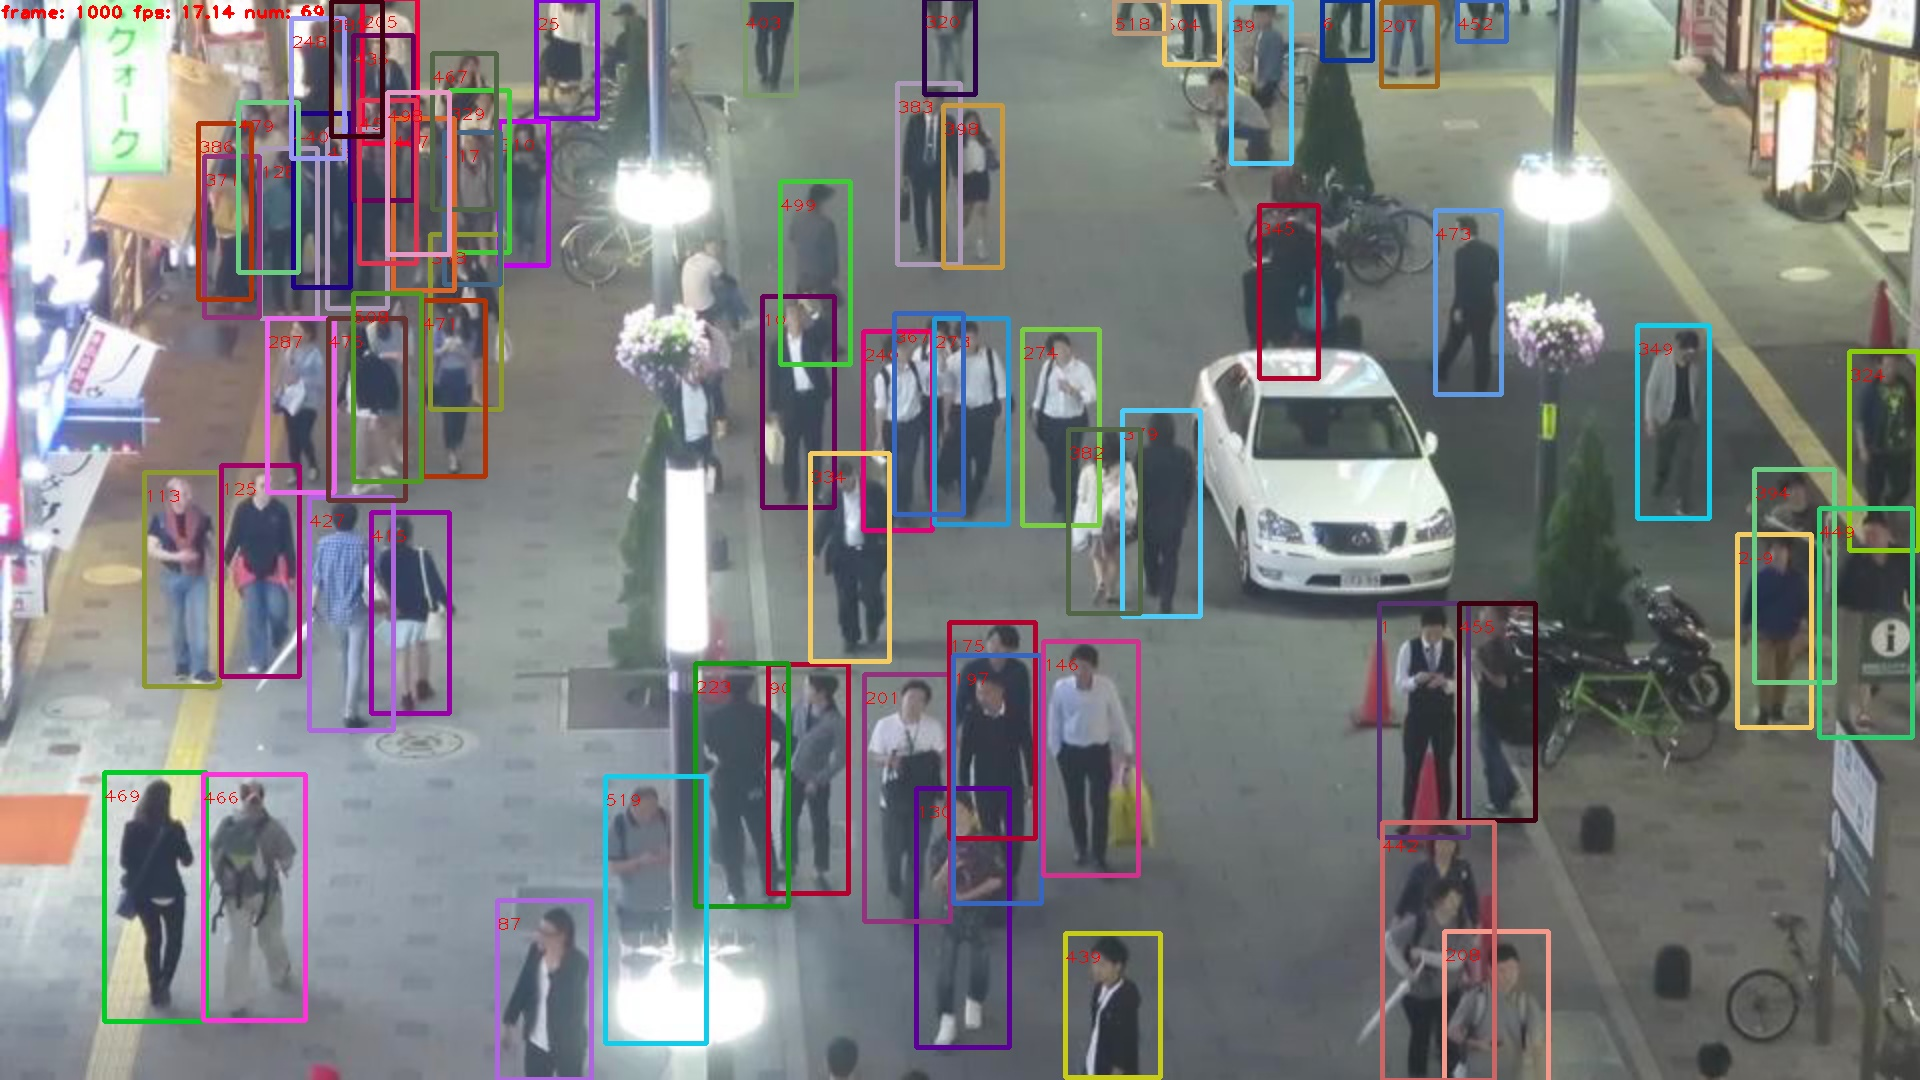
\includegraphics{figures/MOT-16-03_01000.jpg}
				}
				%\includegraphics[scale=1.0]{figurefile}
				\caption{多目标跟踪示例}
				\label{fig:campus}
			\end{figure}
		\end{column}
		\hfill%
		\begin{column}<0->{.65\textwidth}
			\begin{itemize}
				\item<1-> 复杂场景下的多目标跟踪是计算机视觉领域中基础且重要的研究方向
				\begin{itemize}
					\item<1-> 也是全球大学、研究所和公司所亟待解决的核心问题
				\end{itemize}
				% 数字表示出现的顺序
				\item<1-> 主要的应用领域
				\begin{itemize}
					\item<1-> 智能视频监控
					\item<1-> 智能驾驶
					\item<1-> 智能机器人
					\item<1-> 体育视频分析
				\end{itemize}
			\end{itemize}
		\end{column}%
	\end{columns}
\end{frame}


\begin{frame}
	\frametitle{主要问题和挑战}
	\begin{columns}[T] % align columns
		\begin{column}<0->{.40\textwidth}
			\begin{figure}[thpb]
				\centering
				\resizebox{1\linewidth}{!}{
					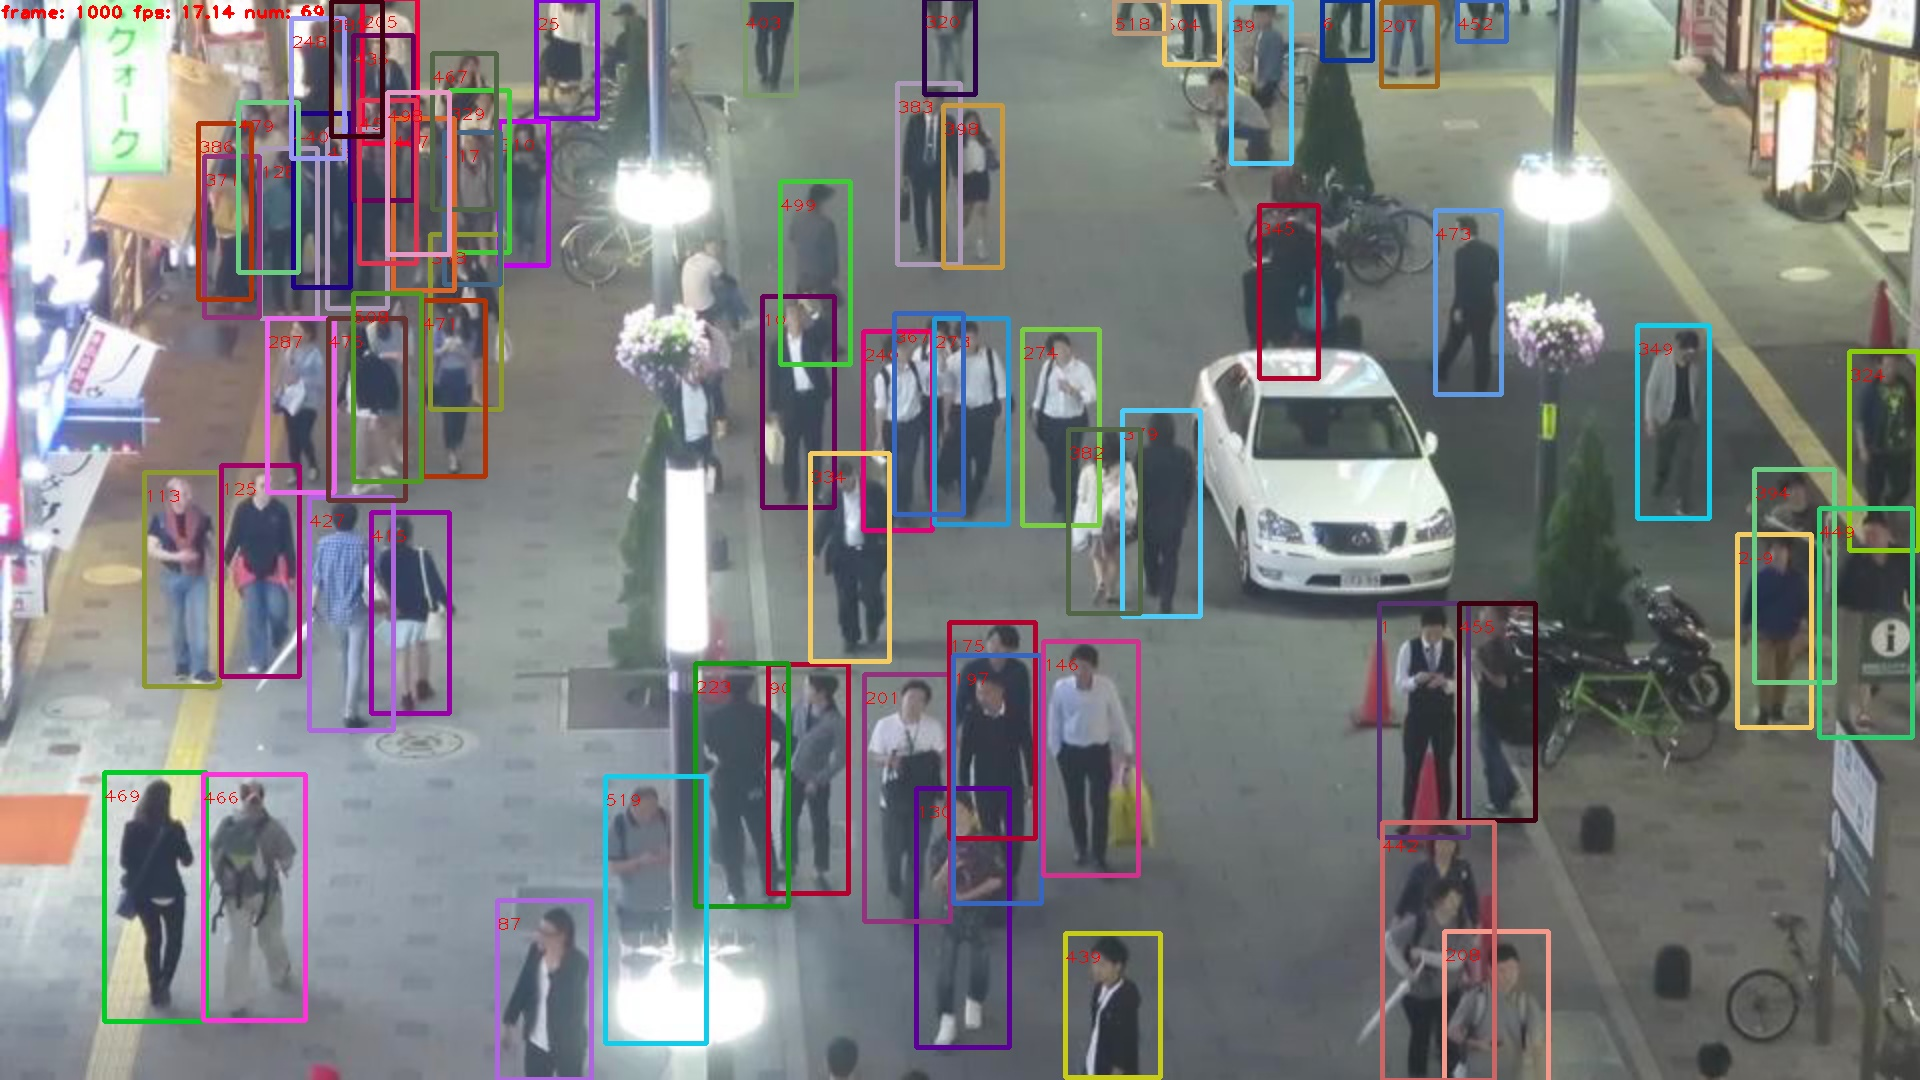
\includegraphics{figures/MOT-16-03_01000.jpg}
				}
				%\includegraphics[scale=1.0]{figurefile}
				\caption{多目标跟踪示例}
			\end{figure}
		\end{column}
		\hfill%
		\begin{column}<0->{.65\textwidth}
			\begin{itemize}
				\item<1-> 单目标跟踪算法扩展到多目标场景中的问题
				\begin{itemize}
					\item<1-> 模型复杂程度和可理解性问题
					\item<1-> 跟踪漂移问题
				\end{itemize}
				\item<1-> 基于检测的数据关联多目标跟踪算法的缺陷
				\begin{itemize}
					\item<1-> 时空特征建模的复杂性问题
					\item<1-> 检测和跟踪任务相互独立问题
				\end{itemize}
			\end{itemize}
		\end{column}%
	\end{columns}
\end{frame}


\begin{frame}
	\frametitle{本文的解决方案}
	\begin{columns}[T] % align columns
		\begin{column}<0->{.40\textwidth}
			\begin{figure}[thpb]
				\centering
				\resizebox{1\linewidth}{!}{
					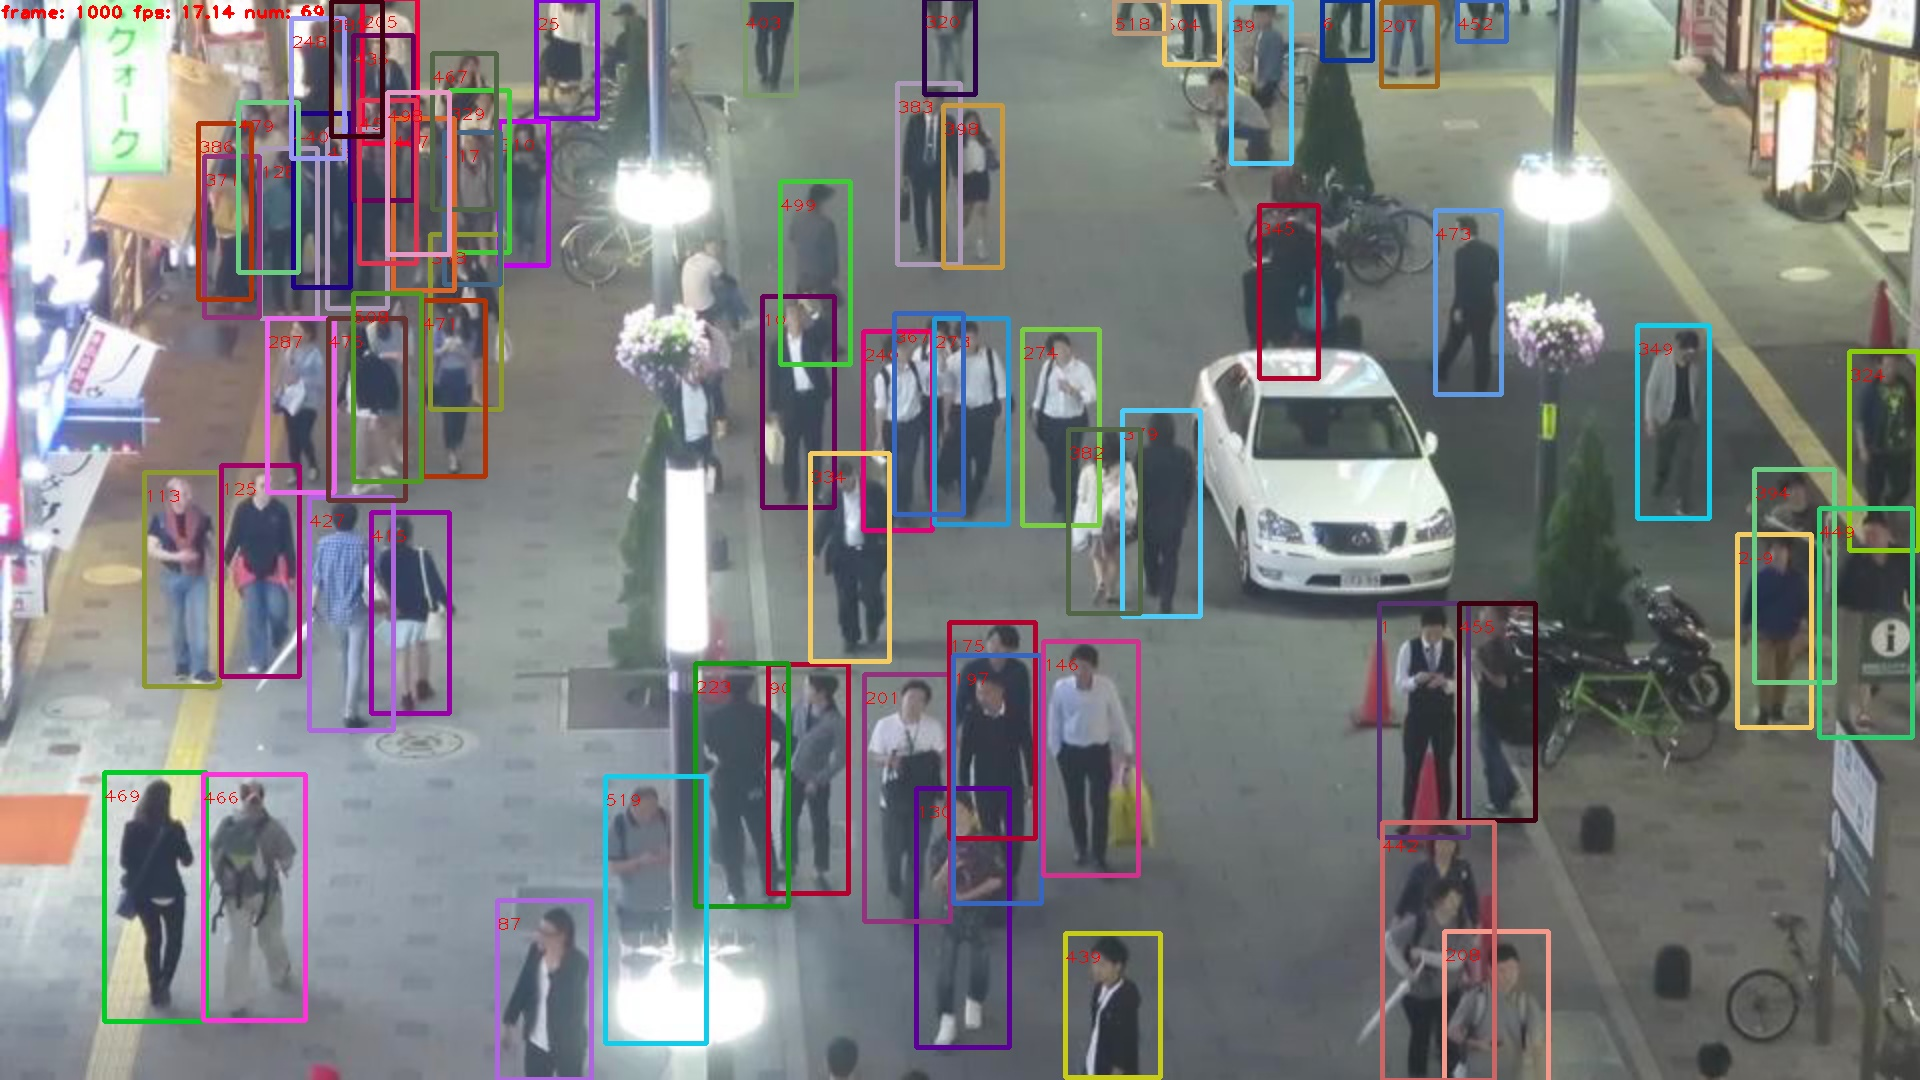
\includegraphics{figures/MOT-16-03_01000.jpg}
				}
				%\includegraphics[scale=1.0]{figurefile}
				\caption{多目标跟踪示例}
			\end{figure}
		\end{column}
		\hfill%
		\begin{column}<0->{.65\textwidth}
			\begin{itemize}
				\item<1-> 神经解剖对齐的类脑跟踪模型,来进行单目标跟踪
				% 2,3都是解决时空特征建模问题 + 漂移
				\item<1-> 跨时范围的全局注意力的模型,提升关联效果并解决漂移问题
				\item<1-> 时空互学习方法,以解决当前和历史特征不平衡的问题
				\item<1-> 端到端模型架构和训练方法,来联合检测和跟踪
				
			\end{itemize}
		\end{column}%
	\end{columns}
\end{frame}
			\section{类脑注意力机制}
\subsection{平滑跟踪大脑皮层通路解剖对齐的视觉跟踪模型}


\begin{frame}{DNN 和带有BTS的神经解剖学对齐之间的协同设计}
	\begin{figure}[!t]
		\centering
		\includegraphics[width=4.5in]{../figures/C2Fig/introduction.pdf}
		%		\caption{DNN 和带有BTS的神经解剖学对齐之间的协同设计}
		\label{ch2_introduction}
	\end{figure}
\end{frame}


\begin{frame}{类脑视觉目标跟踪的网络架构}
	\begin{figure}[!t]
		\centering
		\includegraphics[width=4.5in]{../figures/C2Fig/pipeline.pdf}
		%		\caption{类脑视觉目标跟踪的网络架构}
		\label{ch2_pipeline}
	\end{figure}
\end{frame}


\begin{frame}{大脑——神经网络中各个模块的建模}
	\begin{columns}[T] % align columns
		\begin{column}<0->{.40\textwidth}
			\begin{block}{运动信号处理}
				视网膜
				\begin{itemize}
					\item<0-> $ f_t = M_t^y F_t (M_t^x)^T $
				\end{itemize}
				
				腹侧通路
				\begin{itemize}
					\item<0-> 卷积神经网络
				\end{itemize}
				
				背侧通路
				\begin{itemize}
					\item<0-> $ \left\{ \phi _t ^i \right\}_{i=1}^N = \text{FC}(\alpha_t) $
				\end{itemize}
				
				腹/背侧整合
				\begin{itemize}
					\item<0-> $ m_t = \text{FC}(conc(v_t \odot d_t)) $
				\end{itemize}
			\end{block}
			
		\end{column}
		\hfill%
		
		\begin{column}<0->{.65\textwidth}
			\begin{figure}[!t]
				\centering
				\includegraphics[width=2.8in]{../figures/C2Fig/pipeline.pdf}
				%			\caption{类脑视觉目标跟踪的网络架构}
			\end{figure}
		\end{column}%
	\end{columns}
	
\end{frame}


\begin{frame}{大脑——神经网络中各个模块的建模}
	\begin{columns}[T] % align columns
		\begin{column}<0->{.40\textwidth}
			
			\begin{block}{运动信号转化}
				额叶视区
				\begin{itemize}
					\item<0-> $ h_t, o_t = \text{LSTM}(h_{t-1}, m_t) $
				\end{itemize}
				
				脑干和小脑
				\begin{itemize}
					\item<0-> $ \Delta p_t, \Delta a_{t+1}, \alpha_{t+1} = \text{FC}(conc(d_t), o_t) $
					\item<0-> $ a_{t+1} = a_t + tanh(c) \Delta a_{t+1} $
					\item<0-> $ p_t = a_t + \Delta p_t $
					\item<0-> $ \Delta p_t = \Delta p $
				\end{itemize}
			\end{block}
			
		\end{column}
		\hfill%
		
		\begin{column}<0->{.65\textwidth}
			\begin{figure}[!t]
				\centering
				\includegraphics[width=2.8in]{../figures/C2Fig/pipeline.pdf}
				%				\caption{类脑视觉目标跟踪的网络架构}
			\end{figure}
		\end{column}%
	\end{columns}
	
\end{frame}


\begin{frame}{损失函数设计}
	\begin{columns}[T] % align columns
		\begin{column}<0->{.40\textwidth}
			\begin{block}{}
				跟踪损失
				\begin{itemize}
					\item<0-> $ L_t = -\log(\mbox{IoU} ( \frac{p_t \cap \hat{p}_t}{p_t \cup \hat{p}_t} )) $
				\end{itemize}
				
				背侧通路
				\begin{itemize}
					\item<0-> $ L_d = -\log (\frac{a_t \cap p_t}{p_t}) - \log (1 - \frac{a_t \cap F_t}{a_t \cup F_t}) $
				\end{itemize}
				
				腹侧流损失
				\begin{itemize}
					\item<0-> $ L_v = - r(a_t, p_t) \log(d_t) $
				\end{itemize}
				
				辅助损失
				\begin{itemize}
					\item<0-> $ L_a = 
					\frac{1}{2} \left\vert \left\vert \theta \right\vert \right\vert _2 ^2 + 
					\frac{1}{2} \left\vert \left\vert \phi_t \right\vert \right\vert _2 ^2
					- \sum_{i} \log (\lambda_i^{-1}) $
				\end{itemize}
			\end{block}
		\end{column}
		\hfill%
		
		\begin{column}<0->{.65\textwidth}
			\begin{figure}[!t]
				\centering
				\includegraphics[width=2.8in]{../figures/C2Fig/pipeline.pdf}
				%				\caption{类脑视觉目标跟踪的网络架构}
			\end{figure}
		\end{column}%
	\end{columns}
	
\end{frame}


\begin{frame}{大脑数据分析}
	\begin{block}{\textbf{基本思路}}
		\begin{itemize}
			\item<0-> 为了比较DNN 的视觉目标跟踪和人脑平滑跟踪的相似性,首先需要从各种眼球运动中提取平滑跟踪,然后选择相应的大脑区域和激活用于相似性计算。
		\end{itemize}
	\end{block}
	
	\begin{block}{\textbf{实现步骤}}
		\begin{enumerate}
			\item<0-> 视频刺激的运动估计
			\item<0-> 平稳跟踪样本的提取
			\item<0-> 回归变量建模
			\item<0-> 核磁共振数据分析
		\end{enumerate}
	\end{block}
\end{frame}


\begin{frame}{评价指标:类脑跟踪分数}
	为了在统一指标上评估BTN,该指标计算了眼动行为预测性指标和皮层神经皮层
	预测性指标的平均值,眼动行为预测性表示为:
	\[  s_b=\frac{area(S_{roi}^a \cap S_{roi}^b) }  { area(S_{roi}^a \cup S_{roi}^b) }   \]
	皮层神经预测性表示为:
	\[  s_r=\frac{\sum_{i=1}^{n} (y_i-\bar{y}) (y_i^\prime - \bar{y}^\prime) }{\sqrt{\sum_{i=1}^{n} (y_i - \bar{y})^2 (y_i^\prime - \bar{y}^\prime)^2 }}  \]
	总分数 $s_{t}$ 是两个分数的平均值:
	\[  s_{t} = \frac{s_b + s_r}{2}  \]
	\begin{center}
		\textcolor{mymauve}{BTS 的设计没有在各个分数大小上进行归一化,因为归一化可能会惩罚方差较小的分数。}
	\end{center}
\end{frame}


\begin{frame}{实验结果}
	\begin{columns}[T] % align columns
		\begin{column}<0->{.40\textwidth}
			\begin{figure}[!t]
				\centering
				\includegraphics[width=2.0in]{../figures/C2Fig/comp_sim.pdf}
				\caption{BTN捕获的MT/MST神经响应}
			\end{figure}
		\end{column}
		\hfill%
		
		\begin{column}<0->{.65\textwidth}
			\begin{figure}[!t]
				\centering
				\includegraphics[width=2.0in]{../figures/C2Fig/structure_analysis.pdf}
				\caption{BTN架构分析}
			\end{figure}
		\end{column}%
	\end{columns}
	
\end{frame}

\begin{frame}{实验效果可视化}
	\begin{figure}[!t]
		\centering
		\includegraphics[width=4.5in]{../figures/C2Fig/tracking.pdf}
		\caption{在Tracking-Gump 数据集上跟踪测试所提出模型效果的示例}
	\end{figure}
\end{frame}
			\section{全局注意力机制}
\subsection{基于全局注意力的在线多目标跟踪数据关联策略}

\begin{frame}
	\frametitle{主要问题和挑战}
	\begin{columns}[T] % align columns
		\begin{column}<0->{.46\textwidth}
			\begin{figure}[thpb]
				\centering
				\resizebox{1\linewidth}{!}{
					\includegraphics{../figures/C3Fig/tracking_problem.pdf}
				}
				%\includegraphics[scale=1.0]{figurefile}
				\caption{数据关联的动机}
			\end{figure}
		\end{column}
		\hfill%
		\begin{column}<0->{.65\textwidth}
			\begin{itemize}
				\item<1-> 不完美的检测器
				\begin{itemize}
					\item<1-> 如果检测结果不准确、遗漏或错误,则跟踪对象容易丢失
					\item<1-> 可以将单目标跟踪器和数据关联的优点结合在一个统一的框架中来解决这个问题
				\end{itemize}
				\item<1-> 传统的卷积操作只关注局部特征和检测区域
				\begin{itemize}
					\item<1-> 历史轨迹中的不准确和被遮挡的结果很可能会导致单目标跟踪模型的错误更新
					\item<1-> 专注于跨时空范围的全局特征,而不是局部区域的特征。
				\end{itemize}
			\end{itemize}
		\end{column}%
	\end{columns}
\end{frame}


\begin{frame}
	\frametitle{方法框架}
	\begin{columns}[T] % align columns
		\begin{column}<0->{.46\textwidth}
			\begin{figure}[thpb]
				\centering
				\resizebox{1\linewidth}{!}{
					\includegraphics{../figures/C3Fig/MOT_pipline.pdf}
				}
				\caption{在线多目标跟踪流程}
			\end{figure}
		\end{column}
		\hfill%
		\begin{column}<0->{.65\textwidth}
			\begin{itemize}
				\item<1-> 三个子任务
				\begin{itemize}
					\item<1-> 单目标跟踪
					\item<1-> 目标检测
					\item<1-> 注意力关联
				\end{itemize}

				\item <1-> 漂移时需要基于轨迹的重新识别
				\begin{itemize}
					\item<1-> 关键因素是将轨迹的时空特征合并到特征中
					\item<1-> 非局部注意力层引入传统卷积神经网络以学习图像序列的时空依赖性
				\end{itemize}
			\end{itemize}
		\end{column}%
	\end{columns}
\end{frame}


\begin{frame}
	\frametitle{方法框架}
	\begin{columns}[T] % align columns
		\begin{column}<0->{.33\textwidth}
			\begin{figure}[thpb]
				\centering
				\resizebox{1\linewidth}{!}{
					\includegraphics{../figures/C3Fig/attention_network.pdf}
				}
				\caption{全局注意力网络}
			\end{figure}
		\end{column}
		\hfill%
		\begin{column}<0->{.65\textwidth}
			\begin{itemize}
				\item<1-> 全局注意力网络架构
				\begin{itemize}
					\item<1-> 五个非局部注意力层
					\item<1-> 一系列 ResNet-50网络
					\item<1-> 三维平均池化
				\end{itemize}

			\end{itemize}
		\end{column}%
	\end{columns}
\end{frame}


\begin{frame}
	\frametitle{非局部注意力层的细节}
	\begin{columns}[T] % align columns
		\begin{column}<0->{.33\textwidth}
			\begin{figure}[thpb]
				\centering
				\resizebox{1\linewidth}{!}{
					\includegraphics{../figures/C3Fig/attention_layer.pdf}
				}
%				\caption{全局注意力网络}
			\end{figure}
		\end{column}
		\hfill%
		\begin{column}<0->{.65\textwidth}
			\begin{itemize}
				\item<1-> 非局部注意力机制
				\begin{itemize}
					\item<1-> $ C\left(x\right)=\sum_{\forall j}f\left(x_i,x_j\right) $
					\item<1-> $ f\left(x_i,x_j\right)=e^{ \theta \left(x_i\right)^T \phi \left(x_j\right) } $
					\item <1-> $ y^i=\frac{1}{\sum_{\forall j} e^{\theta\left(x_i\right)^T \phi \left(x_j\right)}} \sum_{\forall j} e^{\theta\left(x_i\right)^T \phi \left(x_j\right)} g\left(x_j\right) $
					\item <1-> 最终整个非局部层最终被形式化为 $ Z=W_{Z}Y+X $
				\end{itemize}
				
			\end{itemize}
		\end{column}%
	\end{columns}
\end{frame}


\begin{frame}
	\frametitle{注意力关联}
	\begin{columns}[T] % align columns
		\begin{column}<0->{.46\textwidth}
			\begin{figure}[thpb]
				\centering
				\resizebox{1\linewidth}{!}{
					\includegraphics{../figures/C3Fig/tracking_problem.pdf}
				}
				%\includegraphics[scale=1.0]{figurefile}
				\caption{数据关联的动机}
			\end{figure}
		\end{column}
		\hfill%
		\begin{column}<0->{.65\textwidth}
			\begin{itemize}
				\item<1-> 将跟踪目标的状态定义为:
				\begin{itemize}
					\item<1-> 如果 $ s > \tau_s $ 且 $ o_{m} > \tau_o $,为跟踪状态,否则为漂移。
				\end{itemize}
			
				\item<1-> 历史轨迹 $o_{m}$ 的平均重叠定义为:
				\begin{itemize}
					\item<1-> $ o_{m}=\frac{\sum_{1}^{L} o\left(t_l,D_L\right)}{L} $
				\end{itemize}
				
				\item <1-> 跟踪目标和检测之间的重叠率定义为:
				\begin{itemize}
					\item<1-> 如果 $ \ max \left(IOU \left(t_l,D_l\right) \right) > \tau_o $,$ o \left(t_l,D_L\right) $ 为 1, 否则为 0。
				\end{itemize}
				
				\item <1-> 当前帧 $k$ 中跟踪目标的坐标预测为:
				\begin{itemize}
					\item <1-> $ c_k=c_{k-1}+v_{k-1} $
					\item <1-> 其中速度 $ v_{k-1}=\frac{c_{k-1}-c_{k-K}}{K} $
				\end{itemize}
			\end{itemize}
		\end{column}%
	\end{columns}
\end{frame}


\begin{frame}
	\frametitle{消去实验结果}
	\begin{columns}[T] % align columns
		\begin{column}<0->{.50\textwidth}
			\begin{figure}[thpb]
				\centering
				\resizebox{1\linewidth}{!}{
					\includegraphics{../figures/C3Fig/ablation.pdf}
				}
				\caption{消去实验结果}
			\end{figure}
		\end{column}
		\hfill%
		\begin{column}<0->{.65\textwidth}
			\begin{itemize}
				\item<1-> 消去的模块
				\begin{itemize}
					\item<1-> B1 表示禁用所提出的 NAAN 并使用跟踪分数来关联历史轨迹和当前检测结果。 
					具体来说,将跟踪器的卷积滤波器应用于候选检测,并直接使用置信图中的最大跟踪分数作为注意力关联的外观相似度
					\item<1->B2 表示禁用非局部注意力层,并使用标准的卷积神经网络架构提取历史轨迹段的特征,将其用于轨迹的身份验证
				\end{itemize}
				
			\end{itemize}
		\end{column}%
	\end{columns}
\end{frame}



\begin{frame}
	\frametitle{网格搜索超参数}
	\begin{columns}[T] % align columns
		\begin{column}<0->{.50\textwidth}
			\begin{figure}[thpb]
				\centering
				\resizebox{1\linewidth}{!}{
					\includegraphics{../figures/C3Fig/grid_search.pdf}
				}
				\caption{网格搜索超参数}
			\end{figure}
		\end{column}
		\hfill%
		\begin{column}<0->{.65\textwidth}
			\begin{figure}[thpb]
				\centering
				\resizebox{1\linewidth}{!}{
					\includegraphics{../figures/C3Fig/parameter.pdf}
				}
				\caption{每个超参数对实验性能的影响}
			\end{figure}
		\end{column}%
	\end{columns}
\end{frame}


\begin{frame}{测试效果}
	\begin{figure}[!t]
		\centering
		\includegraphics[width=3.7in]{../figures/C3Fig/tracking_result.pdf}
		\caption{不同环境下的跟踪结果示例}
	\end{figure}
\end{frame}


			\section{时空互表征学习方法}
\subsection{基于时空互表征学习的鲁棒目标关联在线多目标跟踪}


\begin{frame}
	\frametitle{方法动机}
	\begin{columns}[T] % align columns
		\begin{column}<0->{.50\textwidth}
			\begin{figure}[thpb]
				\centering
				\resizebox{1\linewidth}{!}{
					\includegraphics{../figures/C4Fig/introduction.pdf}
				}
				\caption{时空相互学习和鲁棒的目标关联}
			\end{figure}
		\end{column}
		\hfill%
		\begin{column}<0->{.65\textwidth}
			\begin{itemize}
				\item<1-> 检测结果丢失、忽略或不准确
				\begin{itemize}
					\item<1-> 遵循跟踪预测范式,使用最新的高精度单目标跟踪器来缓解。
					\item<1-> 当跟踪的分数低于阈值时,将使用目标关联方法解决漂移问题
				\end{itemize}
				\item<1-> 当前检测结果的时间特征被忽略的问题,即数据关联双方特征的不平衡问题
				\begin{itemize}
					\item<1-> 通过所提出的时空相互学习方法,序列学习网络学习的时间信息被转移到检测学习网络
%					\item<1-> 由于学习到了时间信息,使得当前检测特征对各种复杂环境具有较好的鲁棒性
				\end{itemize}
			\end{itemize}
		\end{column}%
	\end{columns}
\end{frame}


\begin{frame}{数据关联中时空互学习方法的体系结构}
	\begin{figure}[!t]
		\centering
		\includegraphics[width=4.5in]{../figures/C4Fig/network.pdf}
		%		\caption{DNN 和带有BTS的神经解剖学对齐之间的协同设计}
	\end{figure}
\end{frame}


\begin{frame}
	\frametitle{目标关联流程}
	\begin{columns}[T] % align columns
		\begin{column}<0->{.50\textwidth}
			\begin{figure}[thpb]
				\centering
				\resizebox{1\linewidth}{!}{
					\includegraphics{../figures/C4Fig/i2vtesting.pdf}
				}
				\caption{当前检测结果和历史轨迹序列的数据关联流程}
			\end{figure}
		\end{column}
		\hfill%
		\begin{column}<0->{.65\textwidth}
			\begin{itemize}
				\item<1-> 相似性关联
				\begin{itemize}
					\item<1-> 当单个目标跟踪过程变得不可靠时,将跟踪目标标记为漂移状态,并根据历史目标序列与当前检测结果的相似度得分进行检测到序列的目标关联。
				\end{itemize}
				\item<1-> 目标出现和消失
				\begin{itemize}
					\item<1-> 当当前检测结果与所有跟踪目标的重叠率低于阈值时,将被视为新的潜在目标。
					\item<1-> 当单个目标保持漂移状态超过 $\tau_t$ 帧或直接移出视野时,将终止跟踪单目标跟踪过程。
				\end{itemize}
			\end{itemize}
		\end{column}%
	\end{columns}
\end{frame}



\begin{frame}
	\frametitle{实验}
	\begin{columns}[T] % align columns
		\begin{column}<0->{.50\textwidth}
			\begin{figure}[thpb]
				\centering
				\resizebox{1\linewidth}{!}{
					\includegraphics{../figures/C4Fig/ablation.pdf}
				}
				\caption{基础模块的消去实验}
			\end{figure}
		\end{column}
		\hfill%
		\begin{column}<0->{.65\textwidth}
			\begin{figure}[thpb]
				\centering
				\resizebox{1\linewidth}{!}{
					\includegraphics{../figures/C4Fig/T.pdf}
				}
				\caption{在 MOT16 数据集上使用不同 $T$ 的效果}
			\end{figure}
		\end{column}%
	\end{columns}
\end{frame}


\begin{frame}{测试效果}
	\begin{figure}[!t]
		\centering
		\includegraphics[width=3.7in]{../figures/C4Fig/tracking_result.pdf}
		\caption{在基准数据集上的跟踪结果示例}
	\end{figure}
\end{frame}
			% !Mode:: "TeX:UTF-8"

\chapter{联合检测和数据关联的实时在线多目标跟踪方案}
\label{chap:jdan}

% 翻译参考:https://www.pianshen.com/article/20191669270/
\section{引言}
% 摘要
%近年来目标检测方法和数据关联方法取得了巨大的进步,这两种子任务对于一阶段在线目标跟踪必不可少。
%但是传统上这两个分离的模块是分别进行处理和优化,这导致了动态开放的模型设计,并需要冗余的模型参数需要学习。
%除此之外,这个领域中很少关注将两个子任务整合成一个端到端的模型来优化模型。
%在研究中,提出了一个端到端的检测关联网络,训练和推断都是在同一个网络模型中。
%检测关联网络的所有网络层都是可微的,并联合进行优化来学习有区分性的实体特征,同时使用网络输出的分配矩阵来进行鲁棒的多目标跟踪。
%模型直接使用检测和多目标跟踪的真实值所得到的损失来进行模型优化。
%所提出的方法在几个多目标跟踪的数据集上进行评估,与最好的方法相比取得了较好的跟踪性能。

% 引言
% 多目标跟踪简介
近年来目标检测方法和多目标跟踪方法都取得了巨大的进步~\cite{RN1002,RN1215,mahmoudi2019multi}。
在实际的许多应用中都会从多目标跟踪解决方案中受益,比如智能驾驶~\cite{auto_driving}、视频监控~\cite{deep_sort}、行人动作识别~\cite{mot16}等。
目前为了能在视频序列中进行多目标跟踪,按照处理流程可以将主流方法粗略分为两阶段方法和一阶段方法。


%\begin{figure*}[ht]
%	\centering
%	\includegraphics[width=0.7\textwidth]{./figures/C5Fig/end-to-end.pdf}
%	\vspace{0.2em}
%	\caption{端到端的目标检测和数据关联}
%	\label{fig:jdan_end-to-end}
%\end{figure*}

% 两阶阶段方法
两阶段方法~\cite{fang2018recurrent,nonlocal_association,poi} 包括两个互相分离的阶段,第一阶段的目标检测首先在当前视频帧中定位所跟踪的目标的位置和大小,然后在第二阶段的数据关联中抽取目标的再识别特征用于关联当前跟踪目标和历史的的轨迹段。
目前目标检测~\cite{faster,point,redmon2018yolov3}、再识别~\cite{k_reciprocal,expanded_re} 和数据关联~\cite{nonlocal_association}~的研究已取得了巨大的进步,同时也提高了多目标跟踪任务的性能。
然而由于两阶段模型目标特征的提取进行了两次,该方法在实际跟踪应用中并不能达到实时性的要求。

% 一阶段方法
% 两阶段
不同于两阶段方法,一阶段方法~\cite{jde,voigtlaender2019mots} 尝试将在线检测和关联两者集成到一个框架中,
如图~\ref{fig:jdan_consistency}(b)所示,两个子任务可以在目标表征提取中共享模型参数,以降低跟踪成本~\cite{jde,memory_improved}。
然而,几个明显的缺点阻碍了端到端多目标跟踪模型的实现。
首先,与图~\ref{fig:jdan_consistency}(a)所示的两阶段方法相比,目标检测和数据关联之间存在形态差异。
阶段一只涉及单张图像空间信息的处理,阶段二涉及时间序列上的数据关联。
这些差异使得端到端多目标跟踪模型的设计更加困难。
% 一阶段
其次,常见的一阶段方法采用独立的处理模式进行检测和关联,包括训练有效的检测模型,然后使用复杂的关联技巧来生成轨迹。
关联结果很大程度上取决于检测器的精度。
换句话说,检测和关联在训练过程中是相互独立的,
并且无法实现端到端的训练。
导致目标检测的误差会传播到关联阶段,从而降低了多目标跟踪的准确性。
% 端到端训练的数据问题
最后,对于如图~\ref{fig:jdan_consistency}(a)第一阶段的离线检测模块,多目标跟踪数据集中现有的检测结果或标签没有对应的检测网络模型参数用于构建端到端的检测跟踪模型,即检测网络的输出和关联网络的输入之间的边界框不一致阻止了整个端到端多目标跟踪模型中的训练过程。
因此,必须实现两个子模块之间的数据一致性。
此外,随着检测子模块的训练过程的继续,第二阶段预测的边界框没有相应的真实关联标签。

%而一阶段方法~\cite{jde,voigtlaender2019mots}~是在单个网络中执行目标检测和目标跟踪。
%因此,两个子任务可以在目标表征提取中共享模型参数,显著降低多目标跟踪的成本~\cite{jde,memory_improved}。

\begin{figure*}[ht]
	\centering
	\includegraphics[width=1.0\textwidth]{./figures/C5Fig/consistency.pdf}
	\vspace{0.2em}
	\caption{两阶段、一阶段和端到端方法的对比}
	\label{fig:jdan_consistency}
\end{figure*}


受上述分析的启发,本文提出了一个联合检测和关联网络(Joint Detection and Association Network,JDAN)的端到端训练框架来解决上述问题。
该框架主要由三部分组成:检测子模块、联合子模块和关联子模块。
具体来说,首先使用预训练的双流检测网络来提取初始目标候选及其表征。
然后,使用连接子模块来合并两帧之间所有可能的表征组合,以生成混淆张量。
最后,关联子模块将张量转换为关联矩阵,它表示来自两个帧的多个目标之间的匹配关系。
要联合训练前面的子模块,一个挑战在于不一致的目标问题,
与多目标跟踪任务的跟踪真实标签相比,检测子模块可能会在预测目标的位置和大小上和关联子模块所需要的数据不一致。
为了弥合这一差距,所提出的方法放弃了现有的真实跟踪标签,
如图~\ref{fig:jdan_consistency}(c)所示,利用传统的关联方法~\cite{welch1995introduction} 为检测结果生成伪标签,
然后将其输入到关联子模块以生成跟踪结果。
因此,所提出的模型可以以端到端的方式联合训练所有子模块,以生成稳健的一阶段模型。
此外,由于伪标签仅用于训练阶段而不是测试,因此它们对推理阶段的预测速度没有影响。


与之前的一阶段方法不同,所提出的方法可以以端到端的方式联合训练检测子模块和关联子模块,达到了缓解误差传播的目的。
在 MOT15~\cite{mot15} 和 MOT17~\cite{mot16} 数据集上评估所提出的方法,
并发现所提出的方法优于多个在线多目标跟踪器。
除了精度高之外,端到端方法简单且效率高,适合于实时场景的应用。
相信这项研究将对一阶段在线多目标跟踪有很好的启发作用。


总而言之,该工作的主要贡献如下:
\begin{itemize}
	\item 提出了一个端到端的架构来联合处理目标检测和关联,以缓解检测误差的传播问题。 
	该工作是第一次尝试为多目标跟踪任务进行端到端的模型训练。
	\item 所提出的方法使用伪标签来解决对象不一致问题,并提出了一个连接子模块并进行关联预测,并基于这些伪样本产生精确的跟踪结果。
	\item 通过消去研究在多目标跟踪基准数据集上进行了大量实验。
	结果表明,与几种流行的模型相比,所提出的方法可以实现实时在线跟踪,并实现具较好的跟踪精度。
\end{itemize}


\section{相关工作}
本章总结最近多目标跟踪中所取得的进展,将其分为两阶段方法和一阶段方法进行介绍,并分析了这些方法和之前所提方法的优缺点。
 
\subsection{两阶段方法}
传统的多目标跟踪方法~\cite{deep_sort,mahmoudi2019multi,zhou2018online} 通常将目标检测和数据关联作为两个独立的步骤。
首先,利用目标检测器~\cite{he2017mask,redmon2018yolov3} 以边界框的形式找出每一帧中所有的目标,并在原始图像帧中裁剪出检测结果。
第二阶段通常采用一般的数据关联方法,根据检测结果的交并比和外观表征计算相似度矩阵,
然后在视频帧之间进行状态估计~\cite{multi_pattern,local_sparse,dynamic_fusion} 和数据关联~\cite{kuhn1955hungarian,zhou2018online},以产生各个目标的运动轨迹。
已有许多研究~\cite{mahmoudi2019multi}~利用诸如图匹配~\cite{zhou2018online}、循环神经网络~\cite{fang2018recurrent} 等最新的数据关联方法。

两阶段方法的优势在于它能针对每一阶段分别利用最合适的方法来尽可能提高跟踪性能。
除此之外,两阶段多目标跟踪方法根据检测框裁剪视频帧,并在抽取目标特征之前将目标缩放成相同的大小。
这个缩放操作能较好的解决跟踪目标之间的尺度差异。
最终,这个方法~\cite{poi}在多目标跟踪基准数据集上取得了很好的跟踪效果。
然而,两阶段方法由于在目标检测中的特征抽取和目标跟踪中的特征抽取都非常耗时,在没有模型参数共享时该方法非常慢。
因此该方法很难达到实际场景中所需的实时性要求。

\subsection{一阶段方法}
随着深度学习中目标检测、多目标跟踪和多任务学习~\cite{ranjan2017hyperface,kokkinos2017ubernet} 的发展,多目标跟踪研究的一个趋势是将目标检测和目标跟踪组合在一个单独的处理框架中。
主要的思想是在一个单独的模型中利用参数共享减少模型的运行时间,以达到同时进行目标检测和数据关联。
例如,TrackR-CNN~\cite{voigtlaender2019mots} 在 Mask-RCNN~\cite{he2017mask} 的基础之上添加了一个再识别分支来预测边界框和目标特征。
基于 YOLOv3~\cite{redmon2018yolov3} 的 JDE~\cite{jde} 获得了接近视频帧率的跟踪速度。
FairMOT~\cite{fairmot} 发现基于基于锚框的检测器预测出的目标边界框可能会和实际的目标中心没有对齐,这将会产生严重的歧义和许多的身份切换。

然而目前的一阶段多目标跟踪方法没有实现完全端到端的模型,仍然会导致检测器的误差传播到数据关联步骤,不能进行两个任务的联合优化,
为了进一步解决这个问题,该工作提出了一个联合目标检测和目标关联的真正端到端的跟踪方法,在某种程度上提高了在线多目标跟踪的精度和速度。


\section{端到端跟踪框架}
为了介绍所提出的算法,首先介绍网络的处理流程,
然后描述检测子模块的信息,
再介绍所提出的连接子模块和保持数据一致性的策略。
最后,提出关联子模块和在线跟踪策略来进行端到端多目标跟踪。
本章使用了以下符号。

\begin{itemize}
	\item $ A $ 表示关联矩阵,它指定当前帧 $F_t$ 中所有目标与历史帧 $F_{t-n}$ 中所有目标之间的关联概率。
	\item $B_{t-n, t}$ 是作为历史轨迹真实标签和当前帧真实标签之间的二进制关联矩阵。
	\item $D$ 表示偏移头的输出。
	\item $E$ 表示表征头生成的表征图。
	\item $F$、$F_t$ 和$F_{t-n}$ 分别代表任意帧、当前帧和前 $n$ 帧。
	\item $M_t$, $M_{t-n}$, $M_{t-n,t}$ 和 $M_a$ 分别表示当前帧中的表征张量,前 $n$ 帧中的表征张量,当前帧和前 $n$ 帧之间的混淆张量,以及关联矩阵。
	\item $N_m$ 表示每个视频帧中跟踪目标的最大数量。
	\item $R_t$ 和 $R_{t-n}$ 分别是当前帧和前 $n$ 帧中的表征矩阵。
	\item $S_D$、$S_J$ 和 $S_A$ 分别代表目标检测子模块、检测跟踪连接子模块和数据关联子模块。
\end{itemize}


\subsection{方法流程}
本章所提出的联合检测和关联的多目标跟踪流程如图~\ref{fig:jdan_pipeline} 所示。
由分隔 $n$ 个时间戳的一对视频帧 $F_t$ 和 $F_{t-n}$ 被输入主干网络中。
两个输入视频帧被共享参数的双流检测网络所处理,其中每个流是一个检测子模块,通过它们来学习鲁棒且高分辨率的目标表征。
%
骨干网络中的数字表示相对于原始特征的比例,
后面附加了定位头和表征头,用于预测目标边界框和目标表征 $R_t$。
%$R_t$ 是为关联子模块学习的,如 章节~\ref{sec:association_submodule} 中所述。
%
所有目标表征都连接起来形成表征矩阵 $R_t \in \mathbb{R}^{128 \times N_m}$ 和 $R_{t-n} \in \mathbb{R}^{128 \times N_m}$(没有目标的位置占位符用零进行填充),其中 $N_m$ 是输入帧中所允许的最大目标的数量。
然后,将 $R_t$ 和 $R_{t-n}$ 分别沿垂直和水平方向复制 $N_m$ 次,形成 $M_t \in \mathbb R^{128 \times N_m \times N_m}$ 和 $M_ {t-n} \in \mathbb R^{128 \times N_m \times N_m}$。
这些表征张量 $M_t$ 和 $M_{t-n}$ 的一对一组合被连接成一个混淆张量 $M_{t-n,t} \in \mathbb R^{(128+128) \times N_m \times N_m}$。
随后,使用关联预测器将 $M_{t-n,t}$ 转换为关联矩阵 $M_a \in \mathbb R^{N_m \times N_m}$。
同时,通过使用所获得的关联矩阵来回顾历史视频帧并执行在线多目标跟踪。
此外,利用现有的目标检测和数据关联方法来设计满足要求的子模块。
如图~\ref{fig:jdan_consistency}~所示,为了利用检测子模块,对应于基准数据集的未知检测网络实现与提出的检测子模块之间存在许多不一致。
为了解决检测子模块的输出和关联子模块的输入之间边界框位置和大小不一致的问题,首先在训练的第一阶段中训练检测子模块,
然后使用经过训练的检测子模块生成所有边界框,
并利用传统的关联方法在视频中产生轨迹。
因此,在训练的第二阶段中,通过固定检测子模块的参数,可以利用上一步的输出来训练所提出的关联子模块。
然后继续阶段一和阶段二的循环训练迭代,直到损失函数收敛。
最后,在线多目标跟踪是通过使用关联子模块的输出将当前帧与几个单独的历史帧相关联来执行的。
因此,这些策略可以实现两个拆分子模块之间的数据一致性,以完成训练和端到端实时检测跟踪。


\begin{figure*}[ht]
	\centering
	\includegraphics[width=1.0\textwidth]{./figures/C5Fig/pipeline.pdf}
	\vspace{0.2em}
	\caption{联合检测关联的网络架构图}
	\label{fig:jdan_pipeline}
\end{figure*}

\subsection{目标检测子模块}
\label{sec:detection_submodule}
检测子模块将单个视频帧 $F \in \mathbb{R} ^ {W \times H \times 3}$ 作为输入并获得每个视频帧的目标边界框和相应的表征。
特别是,在主干模型中添加了两种类型的预测头。
使用定位头来定位目标边界框。
此外,如图~\ref{fig:jdan_pipeline} 所示,表征头用于计算目标表征,
将其输入到 JDAN 的后半部分以获得每对视频帧的关联矩阵 $M_a$。

\subsubsection{主干网络}
\label{sec:backbone}
主干网络对于多目标跟踪任务至关重要,因为目标表征需要同时利用低分辨率和高分辨率表征来适应各种尺度的跟踪目标。
FairMOT~\cite{fairmot} 注意到深层聚合有利于减少一阶段方法的身份切换次数,因为编解码网络可以有效处理不同的目标大小。
然而,深层聚合在两阶段方法中并不重要,因为边界框通过裁剪和缩放将具有相同的大小。

在本研究中,为了同时考虑模型复杂性和精度,采用了 ResNet-34~\cite{resnet}。
如图~\ref{fig:jdan_pipeline} 所示,利用深层聚合~\cite{point} 的变体作为检测子模块的主干来适应各种尺度的目标。
与原始深层聚合~\cite{dla} 相比,它在低层和高层表征之间有额外的旁路。
另外,上采样过程中的所有卷积块都被可变形卷积模块~\cite{deformable}所替换,因为它可以自适应地适应目标尺寸的变化,
这些修改同样有利于缓解对齐问题。


\subsubsection{定位头}
\label{sec:detection_head}
定位头的输入是骨干网络的输出表征。
每个定位头使用大小为 $3\times3$ 的卷积核和 $256$ 输出通道,然后是 $1\times1$ 卷积以产生定位输出。
具体来说,它会生成一个低分辨率的位置和大小。

首先,使用热力图头来预测目标中心。
当它与真正的中心目标位置重叠时,该头部在某个位置的输出为 $1$。
输出值随着到目标中心位置的距离增加而减小~\cite{cornernet}。
对于视频帧中的真实边界框 $b^i = (x_1^i,y_1^i,x_2^i,y_2^i)$,目标的中心位置为
$ p^i = (\frac{x_1^i+x_2^i}{2}, \frac{y_1^i+y_2^i}{2})$。
因此,通过将中心位置除以下采样因子来计算表征图上的位置:$q^i = \lfloor \frac{p^i}{G} \rfloor $,其中 $G=4$。
形式上,位置 $q \in \mathbb{R}^2$ 处的热图响应定义为:
$r_{q} = \mathop{max}\limits_{i} ( \mathrm{exp}^{-\frac{(q - q^i)^2}{2\sigma ^2}} ) $,
其中 $\sigma$ 是高斯核,它是目标大小的函数~\cite{cornernet}。
根据焦点损失~\cite{lin2017focal} 设计热图损失函数 $ \mathcal{L}_{h} $ 作为训练目标:
\begin{align}
\mathcal{L}_{h} = -\frac{1}{N} \sum _{q} \begin{cases} (1-\hat{r}_{q})^\alpha \text{log}(\hat{r}_{q}), & \text{如果 } r_{q}=1 \\ (\hat{r}_{p})^\alpha \text{log}(1-\hat{r}_{q}) (1-r_{q})^\beta, & \text{否则}
\end{cases}
\end{align}
其中 $N$ 表示当前帧中目标的数量,$\hat{r}_{q} \in [0,1]^{\frac{W}{G} \times \frac{H}{ G} \times C_h}$ 是位置 $q$ 处的预测热图响应,类别号 $C_h=1$ 和 $\alpha, \beta$ 是焦点损失的超参数。

尺寸头用于预测目标围绕其中心位置的宽度和高度。
尺寸头的输出定义为: $\hat{Z} \in \mathbb{R}^{\frac{W}{G} \times \frac{H}{G} \times C_z} $,其中类别号 $C_z=2$ 表示宽度和高度。
虽然定位精度与目标表征没有直接的关系,但它会影响检测子任务的性能。
对于视频帧中的一个真实框 $b^i$,可以根据 $z^i = (x_2^i-x_1^i, y_2^i-y_1^i)$ 得到框的大小,
并且预测的边界框大小定义为 ${\hat{z}}^i$。

此外,FairMOT~\cite{fairmot} 表明具有中心位置的细化边界框对于提高多目标跟踪精度很重要。
骨干网络中的下采样因子 $G$ 将发挥巨大的量化效果。
偏移头用于更准确地检测目标。
虽然检测精度提升的优势微乎其微,但是多目标跟踪中的目标表征是基于极其精确的边界框学习的,因此在这里引入偏移头,
将偏移头的输出表示为 $\hat{D} \in \mathbb{R}^{\frac{W}{G} \times \frac{H}{G} \times C_d} $,其中类别号 $C_d=2$。
表征图上的真实位移表示为: $d^i = \frac{p^i}{G} - \lfloor \frac{p^i}{G} \rfloor $。
将中心位置位移表示为 ${\hat{d}}^i$。
因此,表示尺寸头和偏移头的 $L_1$ 损失表示为:
\begin{equation}
\mathcal{L}_{s} = \frac{1}{N} \sum_{i=1}^{N} \|z^i - \hat{z}^i\|_1 + 
\frac{1}{N} \sum_{i=1}^{N} \|d^i - \hat{d}^i\|_1.
\end{equation}

因此,定位损失 $\mathcal{L}_{p}$ 表示为前两个损失的组合:
\begin{equation}
\mathcal{L}_{p} = \mathcal{L}_{h} + \mathcal{L}_{s}.
\end{equation}


\subsubsection{表征头}
表征头的目的是提取可以区分各种跟踪目标的外观表征。
在理想情况下,不同身份的目标之间的差异大于同一身份目标之间的差异。
为了实现这一目标,骨干网络的输出为检测目标的表征,
生成的表征图为 $E \in \mathbb{R}^{\frac{W}{S} \times \frac{H}{S} \times C_e}$,其中输出通道 $C_e=128$。
通过表征头学习在中心位置 $p$ 的目标的表征 $E_{p}\in\mathbb{R}^{C}$。
将跟踪目标识别视为分类问题。
同时训练数据集中所有相同身份的目标都被视为一个标签。
对于视频帧中的真实框 $b^i$,获得了热图上的目标中心位置 $\hat{p}^i$。
在某个位置学习一个身份表征 $E_{p^i}$ 并输出到一维分类概率向量 $v(k)$,
并将真实分类标签表示为 $u^i{(j)}$。
因此,身份分类损失被构造为:
\begin{equation}
\mathcal{L}_{c} = \frac{1}{N \times J} \sum_{i=1}^{N} \sum_{j=1}^{J} u^i{(j)} \text{log}(v(j)),
\end{equation}
其中 $J$ 是数据集中所有身份的数量。

最后,总的检测损失 $\mathcal{L}_{d}$ 表示为前两个损失的组合:
\begin{equation}
\mathcal{L}_{d} = \mathcal{L}_{p} + \mathcal{L}_{c}.
\end{equation}



\subsection{连接子模块和数据一致性}
JDAN 训练输入是没有目标边界框的当前帧 $F_t$ 和历史帧 $F_{t-n}$。
此外在关联子模块 $S_A$ 的训练中,JDAN 需要一个真实的二进制关联矩阵 $B_{t-n, t}$ 作为历史帧和当前帧之间的真实标签来计算关联损失。
在图~\ref{fig:jdan_pipeline}~的最左边显示了一对 JDAN 的输入图像帧。
下面描述连接子模块的细节和所需要解决的数据一致性问题。


\subsubsection{连接子模块}
在目标检测子模块 $S_D$ 和关联子模块 $S_A$ 之间,所提出的连接子模块 $S_J$ 将当前帧中的目标表征 $R_t$ 沿垂直方向复制到张量 $M_t \in \mathbb{R}^{128 \times N_m \times N_m}$,
并将历史帧中的目标表征 $R_{t-n}$ 沿水平方向复制到张量 $M_{t-n} \in \mathbb{R}^{128 \times N_m \times N_m}$。
随后如图~\ref{fig:jdan_pipeline} 所示,目标表征 $M_t$ 和 $M_{t-n}$ 沿着目标表征的通道方向合并到 $M_{t-n,t} \in \mathbb{R}^{(128 + 128) \times N_m \times N_m}$。
注意到,垂直和水平复制用于尽可能多地将两组目标进行排列组合,这确保了历史帧 $F_{t-n}$ 中的目标可能与当前帧 $F_t$ 中的所有目标相关联,反之亦然。
然后通过包含的关联预测器五个卷积块~\cite{inception} 将扩展的混淆矩阵 $M_{t,t-n}$ 转换为关联矩阵 $M_a \in R^{N_m \times N_m}$。
在表~\ref{tab:compression_net} 中详细描述了关联预测器的有关信息。
%I.C 是每一层的通道数目, 
%O.C 表示输出通道的数目, 
%$Stride$ 表示步长的大小, 
卷积核是 $1 \times 1$ 的卷积核来压缩维度,卷积核的大小表示感受野的大小; 
BN (Y/N) 表示是否使用批量正则化;
ReLU (Y/N) 表示是否使用 ReLU。
步长和填充在空间维度上都是相同的,卷积核的步长代表提取的精度。

\begin{table}[t]
	\centering
	\tabcolsep=3.5pt
	\caption{关联预测器压缩网络框架的详细信息}
	\label{tab:compression_net}
	\tabcolsep=0.15cm
	\begin{tabular}{c|cccccccc}
%		\hline
		\hline
%		\toprule[1.5pt]
		{子模块}	&{索引} &{输入通道数} &{输出通道数} &{卷积核} &{步长} & {填充} &{BN} &{ReLU} \\
		\hline
%		\midrule[1.5pt]
		\multirow{2}{*}{}
		&	1     & 1024  & 512  	& $1 \times 1$ 	& 1 & 0 &	Y	&	Y\\
		&	2     & 512   & 256   	& $1 \times 1$	& 1 & 0 &	Y	&	Y\\
		\multirow{1}{*}{关联预测器}
		&	3     & 256   & 128   	& $1 \times 1$ 	& 1 & 0 &	Y	&	Y\\
		\multirow{1}{*}{}
		&	4     & 128   & 64   	& $1 \times 1$ 	& 1 & 0 &	N	&	Y\\
		&	5    & 64    & 1    	& $1 \times 1$ 	& 1 & 0 &	N	&	Y\\
%		\bottomrule[1.5pt]
		\hline
%		\hline
	\end{tabular}%
\end{table}%


\subsubsection{训练数据的连接一致性}
在连接子模块中,所有目标表征 $R_t$、$R_{t-n}$ 都来自检测子模块,并且可能与多目标跟踪基准数据集上的跟踪真实值存在数据不一致。
因此,很难进行端到端的模型训练。
为了解决这个问题,在该研究中不使用数据集中跟踪的真实值,采用了一种简单而有效的传统关联方法,称为卡尔曼滤波器~\cite{welch1995introduction}来预测轨迹的位置,从而生成目标表征 $R_t$ 和 $R_{t-n}$ 之间的伪关联标签。
根据伪标签得到一个伪关联矩阵 $B_{t-n,t} \in \mathbb{R}^{(N_m+1) \times (N_m+1)}$,其中每个元素 $b_{k,l}$ 表示目标 $k$ 和 $l$ 之间的匹配关系,增加一列/行($B_{t-n,t}$记为“+1”)表示对象消失/出现在当前帧中。
为 $b_{k,l}$ 定义了三个值:$1$ 表示目标 $k$ 和 $l$ 之间的相同身份(称为“伪正对”),$0$ 表示不同的身份(称为“伪负对”) "),$0.5$ 表示不确定。
在具体的实现中,为卡尔曼滤波器中设置了高阈值以减少伪正对的错误匹配,并设置低阈值以增加伪负对的真实不匹配,余下的配对设置为不确定。

%多目标跟踪基准数据集中的真实边界框和所提出的的检测子模块的输出结果在位置和大小上不一致,
%并且在端到端多目标跟踪中所需的多目标跟踪基准数据中的相应检测器模型参数也无法获取到。
%因此如图~\ref{fig:jdan_consistency}所示,利用经过训练的检测子模块提供的边界框和身份轨迹信息以及多目标跟踪基准数据集中的传统关联方法来解决如的真实值边界框不一致的问题。
%有许多不一致的边界框,包括边界框真实值~\cite{dpm,faster,sdp}和所提出的的检测模块在多目标跟踪基准数据集中的输出之间的数量和位置。
%虽然多目标跟踪基准数据集中提供的训练数据缺乏这些检测模型的实现,但有必要实现一个阶段的多目标跟踪,如章节~\ref{sec:two_stage} 和一阶段多目标跟踪。
%
%首先,使用预训练的检测子模块和传统的关联方法在多目标跟踪数据集中生成一系列轨迹。
%然后,利用这些轨迹结果形成二进制关联矩阵 $B_{t-n,t}$ 跟随 章节~\ref{sec:similarity_loss},
%然后利用它来训练关联子模块。
%最后,使用两阶段训练策略,如章节~\ref{sec:two_stage} 中描述的那样训练整个JDAN,在检测子模块的输出和关联子模块。


\subsection{关联子模块}
\label{sec:association_submodule}
JDAN 中的目标关联子模块 $S_A$ 的目的是使用连接的混淆张量计算 $F_{t-n}$ 和 $F_t$ 这两个目标组之间的关联 $M_{t-n,t}$。

\subsubsection{关联预测器}
\label{sec:similarity_estimator}
如表~\ref{tab:compression_net}所示,关联预测器的结构是根据 $M_{t-n,t}$ 和 $M_a$ 的实际含义设计的。
该模块将目标表征的组合 $M_{t-n,t}$ 转换为关联矩阵 $M_a$,表示这些帧间跟踪目标的关联信息~\cite{dan}。
因此,它沿着目标表征的方向使用卷积核大小为 $1\times 1$ 的卷积逐步实现了从 $256$ 到 $1$ 的维度压缩,同时它不会相互影响特征图中的相邻通道。



\begin{figure*}[ht]
	\centering
	\includegraphics[width=1.0\textwidth]{./figures/C5Fig/loss.pdf}
	\vspace{0.2em}
	\caption{目标消失和出现的处理}
	\label{fig:jdan_loss}
\end{figure*}


\subsubsection{关联矩阵} \label{sec:association_matrix}
如图~\ref{fig:jdan_pipeline} 的后半部分所示,通过利用所提出的关联子模块获得帧间关联,并利用每帧中允许的最大目标数 $N_m$ 预测 $F_{t-n}$ 和 $F_t$ 之间的目标关联矩阵 $M_a$。
如章节~\ref{sec:maximum_object} 中所述,在本研究中 $N_m = 150$ 是多目标跟踪数据集的单帧中目标数目上限。
沿水平和垂直方向在目标相似性关联矩阵 $M_a$ 中插入零向量(作为目标占位符)以进行泛化。
这些零出现在 $F_{t-n}$ 和 $F_t$ 之间,因此任何视频帧最终都由 $N_m$ 个目标组成,并且 $M_a$ 的形状是 $N_m \times N_m$。

$M_a$ 中的行表示历史帧中的目标,其中的列表示当前帧中的目标。
$M_a$ 表示具有水平和垂直目标占位符的两个视频帧的关联矩阵。
在 $M_1$ 和 $M_2$ 中,在末尾矩阵附加了一个额外的水平和垂直向量,称为未识别的目标~\cite{dan}。
如图~\ref{fig:jdan_loss} 所示,最后附加的垂直向量负责建模从历史帧 $F_{t-n}$ 中消失的当前跟踪目标,最后一行中附加的水平向量负责建模在当前帧 $F_t$ 中进入视野的新目标。
对于输入的历史帧和当前帧,JDAN 预测得到相似性关联矩阵 $M_a$。
考虑到历史帧和当前视频帧之间的多目标消失和出现,通过向 $M_a$ 添加额外的列和行来设计 $M_1$ 和 $M_2$。
然后,分别对 $M_1$ 和 $M_2$ 进行水平和垂直 softmax 操作,以保证出现和消失的总概率都为 1,裁剪后的矩阵 $A_c$ 和 $A_r$ 用于与真实关联矩阵计算损失 $ L_m $。
最后,总关联损失 $\mathcal{L}_s$ 由 $\mathcal L_m$、$\mathcal L_b$ 和 $\mathcal L_d$ 所构成。
所以所提出的网络可以表示相机视野中多个目标消失和出现。
例如,可以在最后附加的垂直向量中的一行,从 1 变成 0 来表示消失,
并在最后附加的水平向量的列处,从 1 变成 0 表示出现。



\subsubsection{消失和出现} \label{sec:similarity_loss}
可以计算预测的关联矩阵 $M_a$ 和真实的二进制关联矩阵 $B_{t-n,t} \in \mathbb{R}^{(N_m+1) \times ( N_m+1)}$。
关联矩阵的标签最终用于训练所提出的的关联子模块 $S_A$。
然而,$M_a$ 忽略了历史和当前帧之间的目标消失和出现。
因此,利用历史帧和当前帧之间的相似性关联编码来考虑多个目标的消失和出现。

如图~\ref{fig:jdan_loss} 顶部所示,考虑到目标消失,在 $M_a$ 后附加一列以构建 $M_1 \in \mathbb R^{N_m \times (N_m + 1)}$。
扩展矩阵 $M_{1}$ 的第 $m^{\text{th}}$ 行将帧 $F_{t-n}$ 中的 $m^{\text{th}}$ 目标与 $F_t$ 帧中 $N_m+1$ 个的目标进行关联,其中 $+1$ 表示当前帧 $F_t$ 中未检测到的目标。
然后,通过执行 softmax 操作~\cite{train_mot} 对 $M_1$ 的水平方向上的扩展概率向量进行归一化。
因此,输出关联矩阵 $A_{1} \in \mathbb R^{N_m \times (N_m +1 )}$ 的水平向量表示视频帧 $F_{t-n}$ 中所有目标与在视频帧 $F_t$ 中的所有目标之间的关联概率,包括当前视频帧中未识别的目标。
同理如图~\ref{fig:jdan_loss}~底部所示,目标外观是通过向 $M_a$ 附加一行以构建 $ M_2 \in \mathbb R^{ (N_m + 1) \times N_m}$ 而形成的。
然后,对 $M_2$ 执行垂直 softmax 操作得到 $A_2 \in \mathbb R^{(N_m +1) \times N_m}$,其列表示来自视频帧 $F_{t-n}$ 到 $F_t$ 的关联概率~\cite{train_mot}。


此外,向目标关联矩阵 $M_a$ 添加了额外的列和行以获得可理解的损失设计。
关联矩阵 $M_a$ 添加的向量是 ${\bf u} \in \mathbb R^{N_m} = \lambda {\bf 1} $,其中 $\lambda$ 是超参数,${\bf 1}$ 是一个全为 1 的单位向量~\cite{dan}。
添加向量的这种设计意味着所有跟踪目标都有消失或出现的概率。
此外,二进制关联矩阵 $B_{t-n,t}$ 以相同的方式实现。

具体来说,使用方向性损失 $\mathcal L_{d}$ 来抑制消失和出现的错误目标关联:
\begin{align}
\mathcal L_d = \frac{\sum_{i=1}^{N_m} \sum_{j=1}^{N_m+1} \left( \left(-\log { A_1} \right) \odot {B}_1 \right)}{ \sum_{i=1}^{N_m} \sum_{j=1}^{N_m+1} B_1 }  
\notag  \\
+ \frac{ \sum_{i=1}^{N_m+1} \sum_{j=1}^{N_m} \left( \left(-\log { A_2} \right) \odot {B}_2 \right)}{\sum_{i=1}^{N_m+1} \sum_{j=1}^{N_m} B_2},
\end{align}
其中 $B_1$ 和 $B_2$ 分别通过删除 $B_{t-n,t}$ 的最后一个水平和垂直向量来进行定义,
运算符 $\odot$ 表示哈达玛积~\cite{hadamard},
\textit{log} 函数作用于参数中的每个元素。

此外,利用非极大值损失和平衡损失来训练关联子模块~\cite{dan}。
非极大值损失 $\mathcal L_{m}$ 在关联计算的消失和出现中惩罚非最大关联:
\begin{equation}
\mathcal L_m = \frac{ \sum_{i=1}^{N_m} \sum_{j=1}^{N_m} \left( \left(-\log A_m \right) \odot {B}_3 \right)}{\sum_{i=1}^{N_m} \sum_{j=1}^{N_m} B_3}.
\end{equation}
同理,$B_3$ 是同时删除 $B_{t-n,t}$ 的最后一个垂直向量和最后一个水平向量,
$A_m = max (A_c, A_r)$。
\textit{max} 函数也会作用于输入参数的每个元素。
对损失 $L_m$ 进行 $max$ 操作以获得 $A_c$ 和 $A_r$ 中的最大值,
如图~\ref{fig:jdan_loss}~所示,其中 $A_c$ 和 $A_r$ 分别表示矩阵 $A_1$ 和 $A_2$ 通过删除最后一个垂直向量和最后一个水平向量被裁剪到 $N_m \times N_m$ 的维度。
在视频过程中出现的目标数和消失的目标数应该相等,所以平衡损失 $\mathcal L_b$ 惩罚消失和出现之间的任何不平衡:
\begin{equation}
\mathcal L_b =  \sum_{i=1}^{N_m} \sum_{j=1}^{N_m} \lvert A_c^{ij} - A_r^{ij} \rvert. 
\end{equation}

最后,将总关联损失 $\mathcal L_s$ 定义为上述三项损失的总和:
\begin{equation} \label{equ:association_loss}
\mathcal L_{s} = \mathcal L_d + \mathcal L_m + \mathcal L_b.
\end{equation} 
在这里,关联子模块的训练目标是最小化关联损失 $\mathcal{L}_s$。
因此,上述三个损失是有效的,并拟合了真实目标关联。


\subsection{端到端跟踪}
这一部分描述所提出的端到端模型的训练和用法,以及在没有输入边界框的视频序列中执行多目标跟踪的详细步骤。

\subsubsection{两阶迭代段训练}
\label{sec:two_stage}
在该研究中采用迭代训练过程来训练所提出的模型,包括两个步骤:
首先,在几个检测数据集上采用预训练的目标检测模型~\cite{zhang2017citypersons,xiao2017joint,zheng2017person},并根据检测损失 $\mathcal{L}_{d}$ 对其参数进行微调;
其次,利用卡尔曼滤波器~\cite{welch1995introduction} 进行跟踪,得到目标的轨迹和身份标签,以及当前检测结果和历史轨迹之间的伪标签,
并根据方程~\ref{equ:association_loss} 中的 $\mathcal{L}_{s}$ 更新检测子模块和关联子模块。
反复重复上述两个步骤,直到损失 $\mathcal{L}_{s}$ 收敛。
与以前的方法相比,检测误差可以反向传播回来以更新检测子模块和关联子模块,
因此所提出的训练方法可以实现端到端模型训练以缓解误差传播的问题。

%为了验证基于之前的在线多目标跟踪研究所提出的模型 JDAN,它包含两个可训练的子模块,名为检测子模块 $S_D$ 和关联子模块 $S_A$。
%最后,执行端到端推理。
%首先如~\ref{sec:detection_submodule}节所示,使用边界框框和身份信息和检测损失 $\mathcal{L}_{d}$ 来训练定位头和表征头。
%其中一些数据没有身份信息只有真实边界框,但它们可以被用来训练定位头。
%
%然后,根据预训练的检测子模块生成的边界框对多目标跟踪数据集执行传统的数据关联方法,
%并利用输出生成二进制关联矩阵 $B_{t-n,t}$ 作为训练关联子模块 $S_A$ 的真实数据。
%在第二个训练阶段,通过 $S_D$ 固定检测子模块 $S_D$ 的参数与生成的边界框一致,
%并使用关联子模块 $S_J$ 产生的混淆矩阵和传统数据关联方法生成的二进制关联矩阵训练 $S_A$。
%由于使用了预训练的检测子模块和固定参数,第二个训练阶段和端到端推理阶段生成的表征和框是相同的。
%这些策略确保检测子模块生成的边界框和目标表征在第二个训练阶段在 $S_D$ 和 $S_A$ 之间是一致的。


\label{sec:dep}
\subsubsection{模型预测}
尽管 JDAN 中的目标检测子模块在训练时为两个并行分支,但在线多目标跟踪使用的是同一个网络。
这样做是合理的,因为两个并行检测子模块的权重相互共享。
如图~\ref{fig:tracking} 所示,所提出的网络的预测通过有序的方式呈现主要模块。
JDAN 的输入是一个视频帧 $F_t$,尺寸大小为 $1088 \times 608$。
基于根据章节~\ref{sec:detection_head} 预测出的热力图,由热图响应进行非极大值抑制操作以获得最强点,
选择热图最强响应超过极限值的位置。
然后,根据模型推断结果的大小和偏移量预测相应的框。

此外,检测子模块中的表征头学习当前帧和历史帧的目标表征 $R_t$ 和 $R_{t-n}$。
复制并组合这两个表征矩阵为这两个图像的混淆张量 $M_{t-n,t}$。
然后如章节~\ref{sec:similarity_estimator} 所示,张量 $M_{t-n, t}$ 通过关联预测器的前向传播转换为关联矩阵 $M_a$。

\begin{figure*}[ht]
	\centering
	\includegraphics[width=1.0\textwidth]{./figures/C5Fig/tracking.pdf}
	\vspace{0.2em}
	\caption{JDAN 执行在线多目标跟踪的过程}
	\label{fig:jdan_tracking}
\end{figure*}

\subsubsection{在线跟踪}
在初始化跟踪过程并在第一帧中生成表征 $R_0$ 后,可以预测出当前帧目标和响应历史帧目标表征之间的关联矩阵 $M_{t-n:t-1,t}$。
如图~\ref{fig:jdan_tracking} 所示,推断出的关联矩阵通过回顾历史帧信息来刷新先前的跟踪结果。
在输入视频帧 $F_t$ 中,通过 JDAN 中具有单个流检测子模块,并由定位头和表征头分别得到目标框和目标表征。
目标表征 $R_t$ 用于与最近的 $n$ 个历史表征 $R_{t-n:t-1}$ 进行配对,并且每对表征都通过关联预测器来估计相应的关联矩阵 $M_{t-n:t-1,t}$。
此外,表征 $R_t$ 保存到轨迹记录器中用于估计下 $n$ 帧中的关联矩阵。
最后,通过使用预测的关联矩阵将当前图像目标与 $n$ 个历史图像目标联系起来并更新轨迹记录器。

在这里描述了图~\ref{fig:jdan_tracking} 所示的详细在线多目标跟踪过程。
记录器 $T_0$ 具有相同数量的轨迹,因为识别的目标在第一个视频帧 $F_0$ 中被初始化。
此外,每条轨迹都是一个键值对的记录器,其中的每一项都包含视频帧索引和目标表征。
使用 Kuhn-Munkres 方法更新当前帧的轨迹记录器~\cite{Munkres1957},并通过最大化当前目标和历史轨迹的关联,来进行关联推断。
此外,将其记录到累加器 $Y_{t}$ 中。
累积器矩阵中的每个元素都是历史轨迹记录器 $T_{t-1}$ 中的目标与当前帧中的目标的相似度总和。

因此,视频中的每一帧图像仅使用检测子网络提取一次特征。
然而,目标表征被保存并重复使用多次来评估与剩余图像的相似性。
所以基于关联矩阵可能将许多轨迹分配给累积器矩阵中的特定未检测目标列。
这个问题是通过复制累加器矩阵的最后一列来解决的,直到 $T_{t-1}$ 中的每个估计都分配给唯一的一列~\cite{dan}。
因此,该策略能使每个未检测到的轨迹与未检测到的目标相关联。

总之,所提出的检测跟踪器是一种在线多目标跟踪方法,它不利用任何未来信息来预测目标轨迹。
因此,它可以应用于在线应用中。
一个潜在的问题是过长的轨迹可能会导致大量的存储和计算成本。
因此,阈值 $\mu_m$ 用于限制在现有轨迹中查看的历史帧数。
如果轨道中的图像数量超过 $\mu_m$,则最远的目标信息将被丢弃。
此外,如果跟踪目标从视野中消失超过 $\mu_r$ 帧,它将从跟踪列表中删除~\cite{train_mot}。
在提出的多目标跟踪方法中使用这些有物理含义的参数,可以根据运行时内存和计算资源的限制进行更改。

 
\section{实验}
在这一节分三步展示所提出的 JDAN 实验和结果。
首先,介绍了所使用的数据集和所提出模型的实现细节。
其次,分析了不同训练方法在同一多目标跟踪数据集上的性能。
最后,将所提出的方法与经典和最新的多目标跟踪方法进行比较。

\subsection{数据集和度量标准}
基于已有的研究~\cite{jde,fairmot},通过合并来自多个行人检测数据集的训练数据来利用一个大型训练集来训练所提出的检测子模块。
CityPersons~\cite{zhang2017citypersons} 和 ETH~\cite{ess2008mobile} 数据集仅提供框信息,仅可以使用这些数据集来训练定位头。
CUHK~\cite{xiao2017joint}、Caltech~\cite{dollar2009pedestrian}、MOT16~\cite{mot16} 和 PRW~\cite{zheng2017person} 提供了行人边界框和身份信息,便可以联合训练定位头和表征头。
最后,基于训练好的检测子模块和传统的关联方法~\cite{kernelized,fairmot},通过执行多目标跟踪过程构建训练数据来训练目标关联子模块。

在两个不同的多目标跟踪基准数据集 MOT15 和 MOT17 上对所提出方法的各个组件进行了大量的测试。
MOT17 包含七个训练视频和七个测试视频。
MOT16 包含与 MOT17 数据集相同的视频序列。
而 JDAN 的输入是没有检测信息的纯图像。
因此,该研究中只使用 MOT17 数据集。
另外,使用标准多目标跟踪准确度(MOTA)和 多目标跟踪精度(MOTP),
而 IDF1~\cite{ristani2016performance} 综合了 ID 准确率和 ID 召回率。
评估指标还包括 ID\_Sw、ID Precision(IDP)、误报总数(FP)、遗漏目标总数(FN)和碎片轨迹总数(Frag)~\cite{clear}。
在多目标跟踪基准测试中利用这些指标来衡量多目标跟踪性能。

\subsection{实现细节}
\label{sec:implementation_details}
在该研究中使用 PyTorch 1.2.0~\cite{pytorch} 实现所提出的 JDAN,在 Quadro RTX 6000 GPU 上花费 20 小时进行训练。
使用训练数据集来训练所提出的模型,并基于 MOT17 选择所提出网络的超参数。
因为基准数据集 MOT17 的数据规模不大,选择它进行超参数调整。
最后,实验中使用的超参数描述如下。

如章节~\ref{sec:backbone} 中所述,修改后的 DLA~\cite{point} 被用作检测子模块的主干。
使用在微软 COCO~\cite{lin2014microsoft} 上训练的权重初始化检测子模块。
%输入帧缩放到 $1088\times 608$。
%提议的网络的输入帧尺寸为 $1088\times608$。
在将输入帧输入到 JDAN 之前,这些训练和测试样本被重新缩放到指定的大小,表征图的大小为 $272 \times 152$。
如图~\ref{fig:jdan_consistency} 训练阶段一所示,用 SGD 优化器~\cite{sgd} 训练检测子模块 50 次迭代,初始学习率为 $1e-4$,在第 25 和 40 次迭代时乘以 0.1。
%
每帧允许的最大目标数 $N_m$ 设置为 150,最小批次大小 $B$ 设置为 4,迭代轮次设置为 160,单位向量 $\lambda$ 的乘数因子设置为 10。
将历史帧和当前帧 $N_a$ 之间的最大间隙帧数设置为 30。
然后如图~\ref{fig:jdan_consistency} 训练阶段二所示,使用 SGD 优化器~\cite{sgd} 训练关联子模块,其动量和权重衰减分别设置为 0.9 和 5e-4。
以 0.01 的学习率开始训练,并在第 60、100 和 140 次迭代时乘以 0.1。
训练检测子模块和关联子模块时,需要优化超参数 $\mu_r$ 和 $\mu_m$。
使用网格搜索技术选择两个超参数的最佳值,以在 MOT17 验证数据集上获得最佳 MOTA 性能。
利用 $[3, 30]$ 范围内以 3 为步长来构建网格。
因此,在实际跟踪过程中使用这种方法选择了 $\mu_m=15$ 和 $\mu_r=12$。


%\subsubsection{数据增强}
\label{sec:PP}
同时利用了一系列数据增强方法,例如调整图像尺寸、裁剪和像素值抖动等。
首先,使用 1.0-1.25 范围内的随机采样率增加图像帧的大小,并用多目标跟踪训练集中的平均像素值填充扩展图像中的像素。
同时,裁剪了在 0.75-1.0 随机采样范围内的视频帧。
此外,图像中的每个像素值都乘以范围 0.75-1.25 内的随机值。
输出帧转换到 HSV 空间,饱和分量乘以范围 0.75-1.25 内的随机值。
最后参照 SSD~\cite{Liu2016} 将图像变换回 RGB 空间并乘以随机因子样本。
%
注意到历史帧 $F_{t-n}$ 和当前视频帧 $F_t$ 在视频序列中不一定是连续的,
可以让它们有 $n$ 帧的分隔,其中 $n \in [0, N_a-1] $。
然而,所提出的 JDAN 用于关联连续帧中的目标。
使用跳跃的视频帧进行训练有利于在当前帧与一系列历史视频帧之间的数据关联中使用现有的多目标跟踪方法。
以 0.25 的概率对每个轨迹上的历史和当前视频帧进行采样。
然后,这些视频帧被重新调整为指定的大小 $W \times H \times 3$。
同时,使用了概率为 0.5 的水平翻转。
此外,多目标跟踪中使用的训练数据~\cite{mot16,Lyu2017} 缺乏捕捉背景变化、相机失真和许多现实效果以保持多目标跟踪鲁棒性的能力。
在所提出的跟踪方法中,至关重要的是训练数据涉及足够多的不相关跟踪属性,以增强多目标跟踪模型的鲁棒性。
%因此,对多目标跟踪训练数据集进行后续的数据增强。
%
%所有数据增强方法都在章节~\ref{sec:implementation_details} 中描述
%修改多目标跟踪训练集的方法受到~\cite{Liu2016}的启发,他修改了视频帧以增强训练过程。
%然而,使用先前报告的数据增强方法同步处理历史和当前帧~\cite{Liu2016}。



\subsection{消去实验和讨论}

\subsubsection{训练方法}

\vspace{0.5em}
\renewcommand\arraystretch{1.5}
\begin{table}[htbp]\wuhao
	\centering
	\caption{在 MOT17 基准数据上测试各种训练配置}
	\vspace{0.3em}
	\begin{tabular}
%		{p{3.0cm}<{\centering} p{1.2cm}<{\centering} p{1.0cm}<{\centering} p{1.0cm}<{\centering}
%	p{1.0cm}<{\centering}
%	p{1.0cm}<{\centering}
%	p{1.0cm}<{\centering}
%	p{1.0cm}<{\centering}}
		{c|ccccccc}
%		\toprule[1.5pt]
%		\hline
		\hline
		方法 & MOTA$\uparrow$ & MOTP$\uparrow$ & IDF1$\uparrow$ & MT$\uparrow$ & ML$\downarrow$ &  ID\_Sw$\downarrow$ & Frag$\downarrow$\\
%		\midrule[1.5pt]
		\hline
		{基准模型} & 20.7 & 38.3 & 38.2 & 17.6 & 48.8 & 24,875 & 6,731\\
		{预训练的检测模型} & 34.6 & 42.8 & 40.4 & 19.9 & 46.7 & 18,264 & 4,084\\
		{精调的检测模型} & {42.9} & {52.8} & {48.3} & {21.5} & {45.8} & {13,236} & {3,387}\\
		{精调的关联模型} & {53.0} & {65.2} & {49.7} & {23.4} & {44.3} & {11,875} & {2,845}\\
		JDAN & {\bf58.1} & {\bf79.8} & {\bf59.2} & {\bf27.7} & {\bf32.9} & {\bf6,129} & {\bf1,515}\\
%		\hline
		\hline
%		\bottomrule[1.5pt]
	\end{tabular}
	\label{tab:jdan_training_methods}
\end{table}

在这个阶段,通过使用所提出的几个组件来评估训练过程的效果。
如表~\ref{tab:jdan_training_methods} 所示,执行了五种消去实验,包括基准模型、{预训练的检测模型}、{精调的检测模型}、精调的关联模型和所提出的 JDAN。

基准模型首先采用在微软 COCO~\cite{lin2014microsoft} 上预训练的检测子模块,然后使用生成的伪标签进行关联子模块的微调。
在此基础上,预训练的检测模型表示在检测数据集上重新训练{检测子模块},然后使用在生成的伪标签上训练的{关联子模块}。
考虑到多目标跟踪和检测数据集之间的视觉差距,在多目标跟踪检测数据集上对检测子模块进行微调来提高检测性能,
而精调的关联模型不对{检测子模块}使用多目标跟踪数据集,而是在多目标跟踪数据集上微调{关联子模块}。
JDAN 是在多目标跟踪数据集上对{检测子模块}和{关联子模块}进行端到端训练的整个模型。

表~\ref{tab:jdan_training_methods} 报告了上述训练范式之间的性能比较结果,分析如下:
\begin{enumerate} 
	\item 与{基准模型}相比,{预训练的检测模型}实现了显著的性能提升,MOTA 从 $20.7\%$ 增加到 $34.6\%$,MOTP 从 $38.3\%$ 增加到 $42.8\%$。
	这种改进表明在检测数据集上重新训练{检测子模块}的有效性,因为微软 COCO 上的预训练无法为多目标跟踪任务中的拥挤场景提供准确的行人结果。
	
	\item {精调的检测模型}与{预训练的检测模型}相比进一步提升了 MOTA 性能,MOTP 从 $42.8\%$ 上升到 $52.8\%$,ID\_Sw 从 $18,264$ 降低到 $13,236$。
	这种改进源于在{检测子模块}上使用多目标跟踪数据集来弥合检测和多目标跟踪数据集之间的视觉差距。
	同时,由于使用多目标跟踪数据集更新{关联子模块},{精调的关联模型}也实现了与{精调的检测模型}相同的改进。
	
	\item 从实验结果可以看出 JDAN 以最佳的效果改进了所有指标。
	这种增强不仅归功于精调的{检测子模块},还归功于精调的{关联子模块}。
	具体来说,JDAN 在 MOTA 上达到了 $58.1\%$,这反映了跟踪的准确性。
	如前所述,JDAN 采用{端到端}训练来缓解误差传播问题,并可以获得强大的对象关联能力。
\end{enumerate}

% 
%在这个阶段,使用所提出的子模块评估两个训练阶段的效果。
%并执行各种训练配置,包括“基准模型”、“检测模型训练”、“未精调检测网络”、“未精调关联网络”和提出的 “JDAN” 训练方法。
%这些方法的组件在每种训练方法中仅更改一次。
%将 MOT17 分为 7 个训练集和 7 个验证集来训练目标关联子模块。
%这里没有使用其他更多的数据来验证所提出的训练方法的有效性。
%
%跟踪性能结果显示在表格~\ref{tab:jdan_training_methods} 中。
%在加粗字体中展示了最佳性能。
%“未训练”是基线原始模型。
%“用基础数据训练”是从除 MOT17 以外的各种数据集训练的初始模型。
%“未精调检测网络”是从 MOT17 关联数据而非 MOT17 检测数据训练的微调模型。
%“未精调关联网络” 是从除 MOT17 关联数据之外的多目标跟踪检测数据训练的微调模型。
%JDAN 是在多目标跟踪检测和关联数据上微调的整个模型。
%对“未训练” 和 “用基础数据训练”的分析表明,一定数量的数据会提升整个 MOTA 的性能。
%目标检测和关联极大地受益于更大的训练数据集。
%例如,MOTA 从 $20.7\%$ 增加到 $34.6\%$,
%和 MOTP 从 $38.3\%$ 增加到 $42.8\%$ 对于“用基础数据训练”。
%这些性能改进证明,通过使用更多的训练数据,基本数据集在提高目标检测和关联精度方面具有巨大优势。
%
%“未精调检测网络”仅在“用基础数据训练”的基础上对关联子模块进行微调,获得良好的 MOTA 性能。
%特别是,MOTP 从 $42.8\%$ 显著提高到 $65.2\%$,同时将 ID\_Sw 从 $18264$ 减少到 $11875$。
%跟踪性能表明通过使用更多的训练数据增强了联想能力。
%同时,“未精调关联网络” 与 “用基础数据训练”实现了相同的效果。


\vspace{0.5em}
\renewcommand\arraystretch{1.5}
\begin{table}[htbp]\wuhao
	\centering
	\caption{在 MOT17 数据集上评估目标表征的维度对性能的影响}
	\vspace{0.3em}
	\begin{tabular}
%		{
%			p{2.0cm}<{\centering} p{1.5cm}<{\centering} p{1.3cm}<{\centering} p{1.3cm}<{\centering}
%			p{1.3cm}<{\centering}
%			p{1.3cm}<{\centering}}
		{c|ccccc}
%		\toprule[1.5pt]
%		\hline
		\hline
		特征维度 & MOTA $\uparrow$ & MOTP $\uparrow$ & IDF1 $\uparrow$ & ID\_Sw $\downarrow$ & FPS$ \uparrow$\\
		\hline
%		\midrule[1.5pt]
		1024 & 55.3 & 76.3 & 57.3 & 8,107 & 15.3\\
		512 & 54.7 & 75.1 & 57.1 & 6,810 & 18.7\\
		256 & 56.2 & 78.9 & {\bf59.7} & 7,657 & 19.6\\
		128 & {\bf58.1} & \bf{79.8} & 59.2 & {\bf6,129} & 21.7\\
		64 & 58.1 & 71.6 & 56.7 & 11,675 & {\bf21.9}\\
%		\bottomrule[1.5pt]
		\hline
%		\hline
	\end{tabular}
	\label{tab:jdan_dimension}
\end{table}





%此外,评估了整个训练过程,在 表~\ref{tab:jdan_training_methods} 中命名为 JDAN。
%可以看出,所提出的方法的所有指标都比其他方法更好。
%这种增强不仅归功于微调的检测子模块,还归功于经过训练的关联子模块。
%例如,JDAN 的 MOTA 从 $53.0\%$ 提高到 $58.1\%$。
%特别是 JDAN 表现出最好的 MOTA 性能,因为它获得了强大的目标关联能力。
%此外,JDAN 比“未精调关联网络”具有更强的联想能力。
%因此,认为在 JDAN 中利用关联训练是性能改进的主要来源,因为它可以提高多目标跟踪中的目标关联能力。


\subsubsection{目标表征维度} \label{sec:dimension}
目前已有的行人重新识别方法通常利用高维的目标表征,例如 $1024$,并在没有探究表征维度这个超参数的情况下在数据集上获得了优异的性能。
直到 FairMOT~\cite{fairmot} 发现了表征维度在目标跟踪中起着重要作用。
因为重识别数据集中缺少原始视频帧,所以多目标跟踪方法无法利用它。
故合适的低维目标表征在多目标跟踪中有更好的性能,因为与重新识别任务相比,多目标跟踪缺乏足够的公共训练数据集。
提取低维表征减轻了较小数据集的模型欠拟合问题,并提高多目标跟踪性能。
已有的两阶段多目标跟踪方法不受数据不足的影响,因为它们可以利用丰富的只提供裁剪行人图像的重新识别数据。
而一阶段多目标跟踪方法需要原始未裁剪的视频帧,它无法利用这些重新识别数据,
解决这个数据依赖问题的一种方法是降低目标表征的维数。

在表~\ref{tab:jdan_dimension} 中测试各种维度配置,可以看出当维度从 $1024$ 减少到 $128$ 时,MOTA 不断增加,这证明了多目标跟踪训练数据中低维表征的优点。
此外,当维数减少到 64 时,MOTA 开始减少,因为过低的目标表征已开始导致表征受损。
尽管 MOTA 分数的改进很小,而 ID\_Sw 改进了很多,从原先的 $8107$ 减少到 $6129$,这在提高整体多目标跟踪性能方面起着重要作用。
通过减少目标表征维度,模型运行速度也略有提高。
然而,只有在缺乏训练数据集时,使用低维目标表征才有效。
随着训练数据集的增加,可以缓解表征维度带来的问题。


\vspace{1.0em}
\renewcommand\arraystretch{1.5}
\begin{table}[htbp]\wuhao
	\centering
	\caption{最大目标数阈值 $N_m$ 对目标关联性能的影响}
	\vspace{0.3em}
	\begin{tabular}
%		{
%			p{2.0cm}<{\centering}
%			p{1.5cm}<{\centering}
%			p{1.3cm}<{\centering}
%			p{1.3cm}<{\centering}
%			p{1.3cm}<{\centering}
%			p{1.3cm}<{\centering}
%		}
		{c|ccccc}
%		\hline
		\hline
%		\toprule[1.5pt]
		特征维度 & Det-1024 & Det-512 & Det-256 & Det-128 & Det-64 \\
		\hline
%		\midrule[1.5pt]
		MOTA$^S$ & 56.3 & 55.7 & \bf 57.8 & 58.1 & 53.6 \\
		MOTA$^M$ & \bf{57.8} & \bf 57.9 & 55.3 & \bf 58.4 & \bf 55.3 \\
		MOTA$^L$ & 52.1 & 56.0 & 52.8 & 49.8 & 47.3 \\
		\hline
		ID\_Sw$^S$ & 8,519 & \bf 7,236 & \bf 7,083 & \bf 6,129 & 8,913 \\
		ID\_Sw$^M$ & \bf 2,107 & 8,013 & 7,657 &  6,346 & \bf 6,675 \\
		ID\_Sw$^L$ & 10,397 & 9,281 & 9,597 &  7,475 & 7,286 \\
%		\bottomrule[1.5pt]
		\hline
%		\hline
	\end{tabular}
	\label{tab:jdan_max_obj}
\end{table}




\subsubsection{最大目标数} \label{sec:maximum_object}
由于各种多目标跟踪环境中的目标密度不同,利用适当的最大目标数 $N_m$ 来适应不同的多目标跟踪环境。
与章节~\ref{sec:dimension} 类似,从表~\ref{tab:jdan_max_obj} 中最大目标数的各种配置中可以发现它会影响多目标跟踪性能。
上标~{S} 表示最大目标数为 100; 上标~{M} 表示最大目标数为 150; 上标~{L} 表示最大目标数为 200。
%{Feature dim} 是目标表征维度。
%在加粗中展示了最佳的多目标跟踪性能。
发现当根据章节~\ref{sec:dimension} 将最大目标数设置为 $ 150 $ 且目标表征维度设置为 $128$ 时,可以获得更好的结果。
可以看出过大的最大目标数将导致关联子模块中的欠拟合并降低多目标跟踪性能。





%\vspace{1.0em}
%\renewcommand\arraystretch{1.5}
%\begin{table}[htbp]\wuhao
%	\centering
%	\caption{提出的方法在 MOT15 和 MOT17 基准上与最新的一阶段方法比较}
%	\vspace{0.3em}
%	\begin{tabular}{p{2.0cm}<{\centering} p{1.8cm}<{\centering} p{1.3cm}<{\centering} p{1.2cm}<{\centering}p{1.3cm}<{\centering}p{1.2cm}<{\centering}}
%		\toprule[1.5pt]
%		Benchmark & Tracker & IDF1$\uparrow$ & MOTA$\uparrow$ & ID\_Sw$\downarrow$ & Hz$\uparrow$\\
%		\midrule[1.0pt]
%		MOT15 & JDE \cite{jde} & \bf 66.7 & \bf 67.5 & \bf 218 &  22.5\\
%		& \emph{JDAN}(ours) & { 61.8} & {57.8} & { 494} & {\bf 23.5}\\
%		\hline
%		MOT17 & JDE \cite{jde} & 55.8 & {\bf 64.4} & \bf 1,544 & 18.5\\
%		& \emph{JDAN}(ours) & {\bf 59.2} & 58.1 & {6,129} & {\bf 21.7}\\
%		\bottomrule[1.5pt]		
%	\end{tabular}
%	\label{tab:jdan_onestage}
%\end{table}


\vspace{0.5em}
\renewcommand\arraystretch{1.5}
\begin{table}[htbp]\wuhao
	\centering
	\caption{与其他在线多目标跟踪方法进行比较}
	\vspace{0.3em}
	\begin{tabular}{c|c|cccccc}
%		\hline
		\hline
		数据集 & 方法 & IDF1$\uparrow$ & MOTA$\uparrow$ & MT$\uparrow$ & ML$\downarrow$ & ID\_Sw$\downarrow$ & FPS$\uparrow$\\
		\hline
		MOT15 
		& MDP\_SubCNN\cite{xiang2015learning} & 55.7 & 47.5 & 30.0\% & 18.6\% & 628 & 2.1\\
		& CDA\_DDAL\cite{bae2017confidence} & 54.1 & 51.3 & 36.3\% & 22.2\% & 544 & 1.3\\
		& EAMTT\cite{sanchez2016online} & 54.0 & 53.0 & 35.9\% & 19.6\% & 7,538 & 11.5\\ 
		& AP\_HWDPL\cite{chen2017online} & 52.2 & 53.0 & 29.1\% & 20.2\% & 708 & 6.7\\
		& RAR15\cite{fang2018recurrent} & 61.3 & 56.5 & 45.1\% & 14.6\% & {\bf 428} & 5.1\\
		& {JDE\cite{jde}\textsuperscript{*}} & {56.9} & {{\bf 62.1}} & {34.4\%} & {16.7\%} & {1,608} & {22.5}\\
		& JDAN\textsuperscript{*} & {\bf 61.8} & 57.8 & {\bf 45.3\%} & {\bf 12.9\%} & 494 & {\bf 23.5}\\
		\hline
		MOT17 
		& DMAN~\cite{dual_matching} & 55.7 & 48.2 & 19.3\% & 38.3\% & 2,193 & 0.3\\
		& MTDF~\cite{gm_phd} & 45.2 & 49.6 & 18.9\% & 33.1\% & 5,567 & 1.3\\
		& FAMNet~\cite{famnet} & 48.7 & 52.0 & 19.1\% & 33.4\% & 3,072 & 0.6\\
		& Tracktor++~\cite{tracktor} & 52.3 & 53.5 & 19.5\% & 36.6\% & 2,072 & 2.0\\
		& SST\cite{dan} & 49.5 & 52.4 & 21.4\% & 30.7\% & 8,431 & 6.3\\
		& {JDE\cite{jde}\textsuperscript{*}} & {55.8} & {{\bf 64.4}} & {{\bf 32.8\%}} & {{\bf 17.9\%}} & {{\bf 1,544}} & {18.5}\\
		& JDAN\textsuperscript{*} & {\bf 59.2} & 58.1 & 27.7\% & 32.9\% & {6,129} & {\bf 21.7}\\
		\hline
%		\hline
	\end{tabular}
	\label{tab:jdan_sota}
\end{table}


\vspace{1.0em}
\renewcommand\arraystretch{1.5}
\begin{table}[htbp]\wuhao
	\centering
	\caption{在 MOT17 上每个视频中跟踪效果的详细信息}
	\vspace{0.3em}
	\begin{tabular}{c|ccccccc}
%	\begin{tabular}{p{2.5cm}<{\centering} | p{1.2cm}<{\centering} p{1.2cm}<{\centering} p{1.2cm}<{\centering}p{1.3cm}<{\centering}p{1.2cm}<{\centering}p{1.2cm}<{\centering}p{1.2cm}<{\centering}}
%		\hline
		\hline
		视频序列 & MOTA$\uparrow$ & IDF1$\uparrow$ & MOTP$\uparrow$ & MT$\uparrow$ & ML$\downarrow$ & FP$\downarrow$ & FN$\downarrow$\\
		\hline
%		\midrule[1.0pt]
		MOT17-01 & 55.57 & 53.88 & 80.49 & 33.33\% & 20.83\% & 249 & 2,507\\
		MOT17-03 & 77.09 & 73.35 & 80.69 & 75.68\% & 7.43\% & 10,102 & 13,533\\
		MOT17-06 & 26.68 & 18.91 & 64.54 & 2.25\% & 62.16\% & 6,017 & 8,464\\
		MOT17-07 & 51.53 & 41.13 & 80.60 & 20.67\% & 18.33\% & 512 & 5,767\\
		MOT17-08 & 34.49 & 29.95 & 81.18 & 19.74\% & 38.16\% & 287 & 12,706\\
		MOT17-12 & 50.90 & 54.45 & 80.08 & 28.57\% & 28.57\% & 792 & 3,310\\
		MOT17-14 & 41.83 & 41.56 & 75.13 & 23.17\% & 21.95\% & 739 & 7,696\\
		\hline
		所有 & 58.05 & 59.22 & 79.84 & 27.73\% & 32.99\% & 18,698 & 53,983\\
%		\hline
		\hline	
	\end{tabular}
	\label{tab:jdan_mot17_detailed}
\end{table}



\subsection{性能比较}
在这一部分中,通过与现有的一阶段方法和两阶段方法在内的多目标跟踪方法进行比较来评估和分析所提出的方法。


\subsubsection{两阶段多目标跟踪方法}
本节通过与许多现有的在线多目标跟踪方法进行性能比较来测试和分析 {JDAN}。
为了证明所提出的端到端检测跟踪方法的有效性,在表~\ref{tab:jdan_sota} 中包含了一些关于 MOT15 和 MOT17 的一阶段和两阶段方法。
值得注意的是,两阶段多目标跟踪方法中的跟踪速度(Hz)只包含跟踪阶段而不包括的检测阶段的时间。
然而,在一阶段方法的测试中,所花费的时间同时包括检测和关联。
请注意,用“*”标记了一阶段多目标跟踪方法。
%最好的结果显示在加粗中。
因为不使用多目标跟踪基准数据集中提供的边界框,所以使用了私有检测器。
在 MOT15 和 MOT17 中的测试数据集上展示了多目标跟踪性能。
在评估性能之前,对训练后的模型进行了 6 个迭代轮次的微调。

在 MOT15 和 MOT17 数据上,所提出算法的性能优于其他在线多目标跟踪方法。
与之前的多目标跟踪方法相比,所提出的算法在两个多目标跟踪基准数据上获得了最好的 MOTA 分数,这显示了所提出的方法拥有出色的 MOT 性能,并且所提出的方法计算效率也非常高,所提出的方法获得了接近帧率的跟踪速度。
相比之下,许多高性能方法,例如~\cite{fang2018recurrent,poi},其预测速度低于本章所提出的方法。


\subsubsection{一阶段多目标跟踪方法}
在之前的研究中,只有 TrackR-CNN~\cite{voigtlaender2019mots}、JDE~\cite{jde} 和 FairMOT~\cite{fairmot} 都使用了行人检测和表征学习。
但是 TrackR-CNN 需要额外的图像分割真实标签,并在图像分割问题中使用不同的方法衡量跟踪性能。
%此外,由于使用传统跟踪生成关联数据并训练的关联子模块,因此跟踪精度自然会低于之前开发的方法。
因此,在研究中,将所提出的方法与 JDE 进行比较,只是为了证明提出的端到端检测跟踪方法的有效性。

为了进行合理的评估,使用了 JDE~\cite{jde} 中用于描述的类似数据集,但是没有使用 MOT16 数据集,因为它与 MOT17 具有相同的视频序列,并且它包含的原始视频帧和 MOT16 没有区别。
还利用了 IDF1~\cite{ristani2016performance} 和 CLEAR 指标~\cite{bernardin2008evaluating} 来评估跟踪性能,跟踪性能见表~\ref{tab:jdan_sota}。
容易看出在 MOT17 数据上,所提出的方法优于 JDE~\cite{jde}。
并且它将 IDF1 从 $55.8$ 上升到 $59.2$,整体提高了多目标跟踪性能,详细地跟踪效果信息如图~\ref{tab:jdan_mot17_detailed} 所示。
多目标跟踪性能证明了一阶段方法的优势。
此外,多目标跟踪速度是该算法进行实际应用的一个非常重要优势。



\section{本章小结}
在本章中设计了一个端到端的框架 JDAN 来缓解多目标跟踪任务的误差传播问题,它可以联合训练检测和关联任务,将目标检测和跟踪同时进行优化,超越现有方法。
从技术实现上讲,使用伪标签来解决目标不一致问题,并设计了一个{连接子模块}以及一个{关联预测器}来产生精确的跟踪结果。
{端到端}的架构非常简单而有效,与现有的多目标跟踪方法相比,它避免了繁琐的手动设置。
在广泛使用的多目标跟踪数基准数据集上进行的一系列实验证明了所提出的方法在精度和效率方面都有很大的优势。
相信这个工作可以启发和激励端到端多目标跟踪任务的进一步研究。

%在本章中,设计了一种端到端方法来联合解决目标检测和多目标跟踪任务。
%超越现有的 JDE 方法~\cite{jde},将目标检测和关联结合到一个单一的神经网络中。
%特别是,负责区分不同目标的目标表征嵌入被提取两次,导致两阶段多目标跟踪的重复计算。
%该工作的实现放弃了目标检测和跟踪中的显式锚点,从而提高了多目标跟踪的性能。
%此外,展示了一种明确且自然的端到端 方法,该方法直接利用目标表征将不同帧中的目标关联起来,
%解决端到端检测跟踪中{检测子模块}的输出与{关联子模块}的输入不一致的问题。
%最后,对广泛使用的多目标跟踪基准进行的大量实验证明了所提出的方法在有效性和效率方面的优越性。
%相信所提出的 {JDAN} 可以鼓励和激发一阶段多目标跟踪任务的新方法。

			% !Mode:: "TeX:UTF-8"

\externaldocument{chap2}
\externaldocument{chap3}
\externaldocument{chap4}
\externaldocument{chap5}




\chapter{智能驾驶场景下的多目标跟踪分析应用验证—— 灵动慧眼系统}

% 参考:
% /data2/whd/win10/doc/paper/doctor/doctor.Data/PDF/2687609247

%6.1  应用问题提出(多目标跟踪分析是场景理解、意图分析、预测决策的基础技术,***参考申报书***)
\section{应用问题背景}
随着国内外汽车产业的发展和城镇化的推进,智能交通技术受到世界各国政府与社会越来越广泛的重视。
2017 年 7 月,国务院颁布《新一代人工智能发展规划》~\cite{new_ai_plan},提出发展智能驾驶技术,建立智能驾驶和车路协同技术体系。
2020 年 2 月 24 日,由国家发改委、工信部、科技布等部委印发的《智能汽车创新发展战略》~\cite{car_plan_11}指出推动与人工智能、通信、互联网等行业进行深度融合,全面加速汽车产业转型。
2020 年 3 月,美国发布《智能交通系统战略规划(2020-2025)明确提出了“加速应用智能交通系统,转变社会运行方式”的愿景。
而我国人口基数大、公路网密集,由于汽车作为人们常用的交通工具,其智能化运行有着巨大的市场潜力。
同时近些年,国家“新基建”战略规划的提出和 5G 通信、人工智能等前沿技术的快速发展,为实现车对外界的信息交换(Vhicle to everything,V2X)环境下“人-车-路-云”协同的智能驾驶提供了很好的政策保证和技术支撑。
同时多目标跟踪算法作为智能驾驶实现的前提和基础,为场景理解、行为预测、意图分析等高层决策提供了强有力的支撑。
%
实现实时的多目标跟踪分析系统不仅可以提高出行的安全、运行的效率,还能加速形成具有自主知识产权的智能驾驶技术新产业集群,具有重大的经济价值和社会意义。


因此,本工作除了前面章节中多目标跟踪算法机理和技术的研究之外,也将所提出的算法在智能驾驶环境进行了工程化落地,开发出一套实时在线多目标跟踪系统——灵动慧眼。
%本项目的基本技术想定包括:智慧公共交通环境具备智能交通基础设施、智能路边单元、云中心等辅助支持,智能客车包括多传感器支持下单车智能“感知-决策-控制”技术手段,也具备V2X通信、“车-路-云”协作等技术条件。


\begin{figure*}[ht]
	\centering
	\includegraphics[width=1.0\textwidth]{figures/C6Fig/introduction.pdf}
	\caption{V2X 环境下“人-车-路-云”协同的智能驾驶跟踪感知系统示意图}
	\label{fig:introduction}
\end{figure*}


%6.2 系统需求分析   (车、路、场景的图)
% 参考:https://baijiahao.baidu.com/s?id=1708958727067894390&wfr=spider&for=pc
\section{系统需求分析}

% 系统的范围
\subsection{系统范围}
开发该系统的目的不仅仅是为了收集并保存相机采集到的实时交通场景下的画面,更是为智能驾驶场景提供支撑,对动态开放的智能驾驶场景进行实时多目标跟踪和分析,最终为行为分析、动作预测等更高层的功能提供支持。
该系统主要是一个基于视频的跟踪和分析平台,提供包括实时视频监控、目标跟踪、目标统计分析等信息。
不仅可以在线浏览和处理实时视频流信息,而且可以进行历史视频和信息的回溯。
利用“人-车-路-云”协同的方案,满足智能驾驶场景下实时感知环境的需求,成为智能驾驶场景中必不可少的模块和基础,提升交通和驾驶环境下的智能化水平。


\subsection{系统功能}
% 系统的功能(需求分析)
该系统主要的功能是为智能驾驶系统提供一套高效的感知平台,
如图~\ref{fig:introduction}所示为 V2X 环境下“人-车-路-云”协同的智能驾驶跟踪感知系统的示意图,灵动慧眼有如下几个功能:
\begin{enumerate} 
	\item \textbf{多相机支持}:可以同时配置多个 IP 相机进行同时跟踪,同时可以通过视频流来模拟 IP 相机。
	
	\item \textbf{更低的误报率}:相对于传统多目标跟踪方法,该系统使用本文所提出的多目标跟踪模型进行工程化部署,通过适量采集并标注的数据进行模型微调,并通过使用低置信度跟踪进行过滤。
	
	\item \textbf{结果显示可配置}:显示的检测结果可以进行配置选择,目前主要包括行人和车辆,但是会隐藏平均置信度,并由最常见的检测类别来确定跟踪的类别。
	
	\item \textbf{统计功能}:该系统不仅可以给出每小时的每种类别目标数的统计信息,而且记录每个计数对象交叉点详细信息,比如:相交时间、相交坐标等。	
\end{enumerate}



\subsection{性能需求}
为了实现安全高效的智能驾驶系统,需要该系统提供较高的检测、跟踪和分析的准确度,为了避免危险目标的遗漏,相比于准确率,对算法的召回率提出了更高的要求。
同时为了保证系统能够为高层功能提供实时的感知信息,该系统需要满足基本的实时性需求,实际开发和测试环境中需要达到实时的处理速度。
需要解决一系列提高运行速度的的瓶颈,包括算法性能、硬件加速、网络带宽等。

% 其他需求
%\subsection{其他需求}
%\subsection{运行环境需求}
%本系统的运行环境一般包括:

% 用户和特性
\subsection{用户和特性}
本系统根据最终所具备的功能将用户分为以下几类:
\begin{enumerate} 
	\item \textbf{算法用户}:需要为行为分析、动作预测等高层算法提供支撑;
	
	\item \textbf{监控用户}:为用户提供交通场景下实时和回放的监控画面和跟踪分析信息;
	
	\item \textbf{管理用户}:管理介入到系统中的用户和相机,保证系统的正常秩序;
	
	\item \textbf{系统管理员}:维护该系统的正常运行。
\end{enumerate}

% 系统的风险
%\subsection{系统风险}

%\subsection{安全性需求}
同时该系统在建立和运行的过程中存在一定的安全性风险:可能会产生一定的恶意用户,对建立的这个平台进行不良行为的攻击,由于该实时跟踪分析系统的有效性、实时性优于功能完备性,过多的计算请求会导致合理的跟踪分析功能不能得到实时性的满足,从而对系统的安全性产生侵害。

%\subsection{软件质量属性}




%6.3  系统架构设计   (云-边-端部署场景,软硬件平台,功能模块,功能与性能测试模块等)
\section{系统架构设计}
灵动慧眼系统的核心的实时在线多目标跟踪模块都是基于本文前面章节提出的各个模型和方法进行构建,并采用“人-车-路-云”协同的方式进行设计和部署。
该系统的检测和关联算法为第~\ref{chap:jdan} 章的联合检测关联模型,此外还以第~\ref{chap:btn}~章的类脑单目标跟踪模型作为它们的基础,
使用第~\ref{chap:nonlocal}~章和第~\ref{chap:stml}~章的基于预测的跟踪算法作为对比。
随后对前面在基准数据集上训练好的模型根据自己所采集和标注的部分视频数据进行模型微调,以增强模型的环境适应性,提高系统的跟踪和分析效果。

图~\ref{fig:system_architecture}~展示了灵动慧眼系统的架构设计。
整个多目标跟踪和分析系统主要包括三个组成模块:输入和预处理模块、云端后台处理模块、展示交互模块。
输入和预处理模块是指从各个不同的场景,包括车载摄像头、边缘端的监控摄像头、手持的智能手机摄像头等,使用 IP 相机进行数据的采集并发送到到灵动慧眼系统的流媒体服务器进行初步处理,为多目标跟踪和数据分析提供合适的输入数据。
后台处理模块是该系统最核心的部件,也是本文中各个算法及对比算法实际部署和实现的地方。
最后将跟踪和分析的结果进行页面的展示。

下面对以上每个系统子模块进行详细的介绍。

\begin{figure*}[ht]
	\centering
	\includegraphics[width=1.0\textwidth]{figures/C6Fig/pipeline.pdf}
	\caption{灵动慧眼系统的架构设计}
	\label{fig:system_architecture}
\end{figure*}


\subsection{输入和预处理模块}
由于每个相机所处的空间位置都不同,本系统采用配置好地址和端口的 IP 相机进行输入视频信息的采集,包括智能汽车上的车载摄像头、路边边缘端安装的监控摄像头、行人手持的移动智能手机摄像头等设备,并将不同数据源的视频流数据同时进行处理。
每个车载端或者边缘端的相机都作为一个实时视频数据源服务,通过 RTSP 协议,利用有线或者无线网络实时地向流媒体服务端发送视频流数据。
为了解决流媒体服务器或云端后台处理模块来不及处理视频流数据,导致视频帧堆积的问题,该系统在预处理模块采用生产者消费者模式,建立一个作为临时缓存的生产队列,队列中保存从车载端和边缘端发送过来的视频帧数据。
然后启动一个消费者线程读取生产队列前端中的最新视频帧数据,这样保证后续模块每次处理的都是最新的一帧。
同时将接收到的所有视频数据都保存到数据库服务器中进行备份,以便用户可以通过信息回放功能查看历史视频数据。
服务器端再通过应用程序路由转发给响应的后台处理模块响应的函数进行视频数据的处理,并将最新的视频帧缩放成检测跟踪模型输入所需要的尺寸。


\subsection{云端后台处理模块}
图~\ref{fig:system_architecture} 中的云端后台处理模块简要说明了灵动慧眼系统的实时在线多目标跟踪过程。
对数据传输和预处理模块传输过来的输入图像帧预测其中所有目标的当前目标表征。
然后使用第~\ref{chap:jdan} 章的联合检测关联模型,将当前目标表征和历史表征传递到连接子模块和关联子模块以生成对应的关联矩阵,并通过匹配算法将结果更新到跟踪轨迹管理器中。
跟踪轨迹管理器中存储的历史帧的跟踪信息,以及历史轨迹与当前帧中检测到的目标的相似度之和。
在云端后台处理模块中一个跟踪轨迹对应于一个被跟踪目标的实体。
当接收到一个新的目标表征后,跟踪轨迹管理器将保留表征并将所有历史表征输出到关联子模块以生成每个历史帧和当前帧之间的关联矩阵。
之后更新跟踪轨迹管理器,并生成当前帧中的跟踪结果,传递给展示交互模块。
同时在跟踪过程中将原始视频和所产生的跟踪和以及分析统计信息保存到数据库服务器,用于后面对历史信息进行回放和查询。

该模块使用的联合检测关联模型属于一阶段的端到端在线多目标跟踪模型,其中每个被跟踪目标的外观特征在整个系统的处理流程中只提取了一次,同时将提取到的外观特征保存下来供将来的关联步骤使用。
为了提高系统的响应速度,在测试和部署时使用高性能的计算机硬件进行加速,特别是使用计算能力强的显卡优化联合检测关联模块的计算过程,使灵动慧眼系统能在实际运行中基本达到工程化的实时性要求。
这对于智能驾驶系统的及时感知和预测有着至关重要的作用,提升了系统的实时性和安全性。

为了保证该系统对其他检测跟踪算法的可扩展性,可以使用其他检测跟踪算法替换本文所提出的方法,以便进行不同算法的测试和对比,实现系统模块内的高内聚和模块间的低耦合。
主要可以替换和测试一些经典的检测跟踪算法和最新的且精度较高的算法,测试不同算法在不同驾驶场景下的跟踪和分析效果,便于找出算法的不足之处以便进行优化和改进。



\subsection{展示交互模块}
由于根据函数路由返回的流式响应视频流需要在网页中显示,所以展示交互模块使用客户端浏览器显示跟踪和分析结果的视频流来自动更新页面中的图像元素。
可以使用不同的客户端,比如 PC 终端、智能手机等从 Web 服务器获取跟踪和统计分析信息并进行实时地显示。
在该系统中,对于每个检测并跟踪到的目标都会对当前目标的总计数进行记录的更新。
当相机视野中出现一个新的类别,即每检测到一个新的类别还会创建一个新的类计数器。
灵动慧眼系统除了跟踪和分析常见的行人,还可以通过配置进行比如行人、车辆等多个类别的多目标跟踪和统计分析。
使该系统能很好地对变化中的需求进行适应,以达到更好的应用效果,对高层应用和用户使用提供了更高的支撑。

该模块仅仅用于用户与系统的展示和交互上,对于多目标跟踪的过程和为其场景分析功能的添加只起到调试和显示效果,在真实工程化部署时可以进行配置并省略,以减少系统的开销,提高系统的运行速度和增强实时响应能力。


\subsection{系统部署和性能评测}
灵动慧眼系统的运行环境包括操作系统及其版本,服务器端采用 Ubuntu 18.04 及以上版本,客户端可以为任意的 PC 终端、手机移动端等;
系统数据传输和预处理模块的输入端基于 RTSP 实时流协议使用 IP 相机收集车载端、边缘端以及其他视频数据,并向流媒体服务端发送视频流数据。
服务器端的云端后台处理模块使用 OpenCV、TensorFlow~\cite{abadi2016tensorflow}、Pytorch~\cite{paszke2019pytorch} 等 Python 库进行实现。
整个云端后台处理模块部署在 128G 内存的 20 核且拥有 4 块 RTX 2080 GPU 的高性能服务器上,可以为其他更高级的场景分析和用户浏览提供实时服务。
目前主要的跟踪服务主要运行在云端,并测试多路相机输入时的跟踪情况。
系统展示交互模块的网页前端~\footnote{https://flask.palletsprojects.com/en/2.0.x/}及服务端使用轻量级的 Flask~\footnote{https://github.com/LeonLok/Multi-Camera-Live-Object-Tracking} 框架进行实现。


将高分辨率的单个摄像机流在以 30 FPS 的速度进行流式传输时,在服务器上托管下平均可提供约 15 FPS 的检测跟踪速度。
由于该系统支持多个车载端和边缘端的 IP 相机进行视频流输入,但是服务器资源有限,同时处理多个视频流将会一定程度上降低多目标检测跟踪和分析的速度。
降低处理视频流的分辨率或图像质量将提高系统的运行速度,但同时也会降低检测跟踪的精度。
在基本满足实时性的要求时,需要在速度和精度之间做出权衡,以获得最佳的系统效果。
同时还有很多其他因素会影响灵动慧眼系统的整体性能,比如网络信道质量、带宽等。




%6.4  系统测试 (按照功能、性能指标,分场景(目标密集、目标稀疏;高速、低速;场景清晰,场景复杂等),多个对比算法)
\section{系统测试和验证}
为了说明该系统的有效性,分别从定量和定性两个角度展示灵动慧眼系统的实际效果。
首先进行定量化测试和验证,将本文的方法和一些经典多目标跟踪算法在同样的智能交通场景视频进行多目标跟踪并把结果保存下来,并利用手工标注的方法获得跟踪所对应的真实值,然后如图~\ref{tab:quantitative_test} 所示计算出多目标跟踪性能评价指标,可以看出本文所提出的方法在智能驾驶场景下有较大的优势。

\vspace{0.5em}
\renewcommand\arraystretch{1.5}
\begin{figure}[htbp]
	\centering
	
	\subfigure[动态开放交通场景下车辆的跟踪和统计效果]{
		\begin{minipage}[t]{0.90\linewidth}
			\centering
			\includegraphics[width=1\textwidth]{figures/C6Fig/cidi_car.pdf}
		\end{minipage}%
	}%
	%	\subfigure[With STURE]{
		%		\begin{minipage}[t]{0.48\linewidth}
			%			\centering
			%			\includegraphics[width=1\textwidth]{figures/C6Fig/dongfanghong.pdf}
			%		\end{minipage}%
		%	}%
	
	\subfigure[动态开放场景下行人的跟踪和统计效果]{
		\begin{minipage}[t]{0.90\linewidth}
			\centering
			\includegraphics[width=1\textwidth]{figures/C6Fig/cidi_person.pdf}
		\end{minipage}
	}%
	%	\subfigure[Tracking results with STURE]{
		%		\begin{minipage}[t]{0.48\linewidth}
			%			\centering
			%			\includegraphics[width=1\textwidth]{figures/C6Fig/experiment.pdf}
			%		\end{minipage}
		%	}%
	
	\centering
	\caption{灵动慧眼系统多相机多类型跟踪统计效果展示}
	\label{fig:system_present}
\end{figure}

\vspace{0.5em}
\renewcommand\arraystretch{1.5}
\begin{table}[htbp]\wuhao
	\centering
	\caption{智能驾驶场景下不同方法之间性能的比较}
	\vspace{0.3em}
	%\vspace{0.5em}\wuhao{\textwidth}
	\begin{tabular}{c|cccccccccc}
%		\hline
		\hline
		方法   & MOTA$ \uparrow $ & MOTP$ \uparrow $  & IDF1$ \uparrow $  & IDR$ \uparrow $ & FP$ \downarrow $  & FN$ \downarrow $  & MT$ \uparrow $  & ML$ \downarrow $  & IDS$ \downarrow $  & Frag$ \downarrow $\\ 
		%		\midrule[1.0pt]
		\hline
		PHD\_DAL~\cite{2019Online}    &36.9 &68.1 &29.5 &37.2 &150 &452 &6.5 &53.7 &375 &438\\
		HISP~\citep{baisa2021robust}   &37.2 &70.8 &30.1 &39.5 &150 &366 &8.7 &43.1 &247 &347\\
		GMPHD\_ReId~\citep{baisa2021occlusion}  &37.3 &73.3 &41.2 &30.8 &114 &252 &8.6 &42.8 &165 &157\\
		DASOT17~\citep{chu2020dasot}   &40.1 &71.1 &36.2 &27.9 &217 &363 &8.2 &39.3 &121 &240\\
		NAAL   &45.2 &\bfseries73.8 &\bfseries50.1 &40.9 &151 &215 &9.2 &41.3 &92 &107\\
		STURE     &47.1 &73.2 &48.2 &34.6 &\bfseries51 &\bfseries123 &\bfseries11.2 &41.0 &73 &35\\
		JDAN     &\bfseries53.7 &73.5 &41.2 &\bfseries47.2 &143 &493 &9.16 &\bfseries36.8  &\bfseries31 &\bfseries24\\
		\hline
%		\hline
		%		\bottomrule[1.5pt]		
	\end{tabular}
	\label{tab:quantitative_test}
\end{table}

如图~\ref{fig:system_present} 所示按照功能、场景、算法等方面展示系统验证的效果。
选取了两个典型的实时场景进行多目标跟踪和统计的功能验证效果展示,其中图~\ref{fig:system_present}(a) 展示了动态开放十字路口的多目标车辆跟踪和统计的效果,图~\ref{fig:system_present}(b)展示了典型室外场景下的多目标行人跟踪和统计的效果,表明该系统在典型动态开放场景下能实现同时进行不同类型目标的跟踪和分析,很好地实现了该系统的功能需求。


\vspace{0.5em}
\renewcommand\arraystretch{1.5}
\begin{figure*}[ht]
	\centering
	\includegraphics[width=0.8\textwidth]{figures/C6Fig/system_test.pdf}
	\caption{灵动慧眼系统在具有挑战性的环境下的测试}
	\label{fig:system_test}
\end{figure*}

% Faster RCNN~\cite{b8} 和 YOLOv3~\cite{redmon2018yolov3}
图~\ref{fig:system_test} 中显示了该系统在具有各种挑战条件下进行响应的验证,选取了阴天或者雨天等光照不足的天气情况作为基本背景,以测试该跟踪分析系统应对复杂极端情况的能力。
图中第一行的两图分别表示在目标稠密和稀疏的交通场景下系统的运行效果,第二行分别表示智能汽车在高速和低速运动时的跟踪和分析结果,第三行表示使用其他方法进行测试时的效果,这里使用经典的 PHD\_DAL~\cite{2019Online} 和 DASOT17~\citep{chu2020dasot} 作为测试对比方法,这种情况下存在一定的检测和跟踪错误,反过来证明本文所提出的方法在应对有挑战的现实环境下具有较强的鲁棒性。

以上测试和验证效果均表明该系统在现实动态开放场景下能取得不错的性能并产生较大的实际应用价值。



%6.5  本章小结(应用效果,如何服务于其他模块;验证前面算法效果;从应用的角度强调内脑计算分析的有点)
\section{本章小结}
基于本文研究工作所开发的灵动慧眼系统,实现 V2X 智能驾驶环境下“人-车-路-云”的协同感知,不仅能够自动进行目标的检测和跟踪,还能提供所关注环境中的统计信息,如目标交汇、速度、方向等,同时在实际测试过程中表现出较好的效果和实时性。
该系统不仅仅提供自动实时地监控服务,极大地减少了人力消耗,同时为人和其他算法进行高层次的分析和决策提供助力,增强驾驶场景下的智能化水平,帮助智慧城市的实现。
该系统以人工智能作为促进社会智能化发展的新手段,为社会的文明和进步做出贡献。





			% !Mode:: "TeX:UTF-8"

\addcontentsline{toc}{chapter}{结论与展望} %添加到目录中\quad 
\chapter*{结论与展望}

在动态开放的多目标跟踪环境中,多目标跟踪模型的可解释性和关联特征建模的复杂性是制约跟踪算法取得好的跟踪效果的主要原因。
因此,本文根据跟踪模型在动态开放场景中的可解释性和关联特征建模复杂等挑战进行研究,设计了一系列模型来有针对性地处理这两个问题来提升多目标跟踪模型的效果。
下面简要说明本文所取得的成果以及将来的研究展望。

一、本文的主要成果

根据神经科学、深度学习、计算机视觉等领域的思想和方法来应对动态开放跟踪场景下多目标跟踪所存在的可解释性和关联特征问题,取得的主要成果包括:

(1)
提出了一种类脑跟踪模型,来解决传统深度跟踪模型进行视觉目标跟踪和人类大脑处理平滑跟踪机理之间的矛盾。
从网络结构、中间激活和行为输出三个角度来设计和衡量类脑模型的类脑相似性。
在网络结构方面,通过将平稳跟踪相关脑区映射到不同深度模型的模块,使深度网络结构与人类大脑结构一致,达到理解目前日益加深的深度跟踪模型的作用,同时能去除冗余的模块,加快跟踪模型的运行速度,以达到应用实时性的要求。
%首先,提出一种和人脑解剖结构对齐的深度跟踪神经网络模型,使其更加符合大脑皮层平稳跟踪的解剖通路。
在中间层激活方面,将大脑皮层中 MT/MST 的激活与类脑神经网络动态滤波网络层的激活进行对比,发现了它们之间激活的相关性,为模型的运动感知提供了具体的解释,激活的相似性同样为脑机接口的应用提供了可能。
在行为输出方面,主要考虑了人眼注意力范围和类脑跟踪网络输出的边界框之间的交并比。
并从中间层激活和行为输出方面定量化衡量了大脑皮层处理模式和类脑跟踪模型处理之间的相似性,发现类脑模型能较好地模拟大脑处理视觉目标跟踪的机理和行为。
所提出的类脑模型不仅能够很好地符合计算机视觉对目标跟踪的工程需求,还能对模型所具有的结构和输出行为做出合理地解释,拉近神经科学和计算机科学之间的距离,使大脑的理解和神经网络的设计得以相互促进。
%最后,设计了一种新颖的度量方法来衡量类脑跟踪模型与人脑皮层响应和人眼行为之间的相似性,以评估所提出模型的类脑性能。
%通过在公共的数据集上进行实验,深度分析了类脑模型的跟踪性能与大脑皮层响应和人眼行为之间的相似性,验证了所提出的类脑跟踪模型不仅能够取得比较好的跟踪效果,而且表明所设计的模型和人脑大脑处理平稳跟踪任务时的相关性,并从类脑模型结构、皮层激活响应和人眼行为等方面进行了解释。

(2)
提出了一种综合时空特征的非局部注意力模型。
%为了应对多目标跟踪环境种目标外观变化、频繁遮挡等问题,解决当前视频帧的检测结果与历史轨迹段进行数据关联时,当前检测结果缺乏时间特征和传统卷积操作提取特征的局部性,提出全局注意力模型,以达到更好的关联效果。
由于传统的卷积神经网络在提取视频序列的特征时不能很好地同时考虑时间和空间上的特征,无法处理动态开放场景下各种复杂的挑战,
本文提出了一种在卷积神经网络中加入全局注意力层来自适应地学习视频序列中的时空非局部特征,由于考虑了整个跟踪轨迹的全局信息,能够很好地抑制其中检测结果不准确等情况。
并使用了预测跟踪范式来很好地处理了检测器的检测结果不准确和没有利用目标的运动信息等问题,在单目标跟踪不可靠时使用注意力关联策略来对跟踪漂移进行纠正,较好地处理了目标遮挡和跟踪轨迹中存在的异常样本对跟踪性能的损害。
同时利用一系列数据增强方法和训练策略来进行模型的训练,经过各种消去研究和实验分析证明了非局部注意力机制和预测跟踪范式整体提高了动态开放场景下多目标跟踪的性能。
%,以抑制部分检测不准确和遮挡的挑战。
%其次,还提出了一种注意力关联方法来处理多目标跟踪过程中序列的相关性和遮挡,以缓解历史轨迹中不可靠样本对关联的影响。
%最后,提出一种关联训练方法和数据增强策略解决训练数据不足的问题。
%在基准数据集上进行一系列实验证明了所提出的非局部注意力机制和注意力关联网络可以取得较好的的跟踪结果。

(3)  
提出了一种时空互学习模型来处理多目标跟踪数据关联时的特征不平衡问题。
当进行数据关联时当前帧的检测结果缺少历史轨迹的时间信息,导致不能进行有效地数据关联,严重损害了多目标跟踪的性能。
%%为了解决当前检测结果缺少时间信息和历史轨迹序列特征之间的差异问题,使当前候选检测在进行数据关联时能够很好地进行关联。
而所提出的时空互表征学习方法将检测集的空间特征和序列集的时空特征置于同一时空互表征空间,并通过选择反向传播策略,使检测学习网络能够很好地学习到历史轨迹序列的时间特征,增强当前检测的表达能力,
并通过设计合理有效的损失函数来提升模型的辨别能力,使时空互表征学习能够更好地进行。
并利用单目标跟踪和数据关联方法解决了检测结果不完美和单目标跟踪器漂移的问题,
经过一系列的消去实验和性能测试表明所提出的时空互表征学习方法能很好地解决在线多目标跟踪数据关联中的特征不平衡问题,并提升了跟踪性能。
%首先,本文提出了一种时空互表征学习框架来解决当前检测结果仅包含的空间信息和历史轨迹序列包含时空信息之间的特征不平衡问题。
%其次,为了增强所提出方法的互学习和特征区分能力,设计了三种损失函数:交叉损失、模态损失和相似性损失,有助于检测学习网络获得历史序列中的时间特征。
%最后,设计了一种基于预测的多目标跟踪范式,通过使用时空互增强得到的特征来缓解单目标跟踪器的漂移现象。
%通过在多目标跟踪基准数据集上执行一系列消去试验,证明了该方法能够在复杂的跟踪场景下取得非常不错的跟踪性能。

(4)  
提出了一种联合目标检测和数据关联的在线多目标跟踪方法,解决了传统计算机视觉将检测和跟踪分开处理对目标特征重复提取的问题。
并利用检测子模块进行目标检测和特征的提取,连接子模块来进行前后帧目标特征的连接和融合,关联子模块来进行关联矩阵的预测,并进行在线多目标跟踪。
在此过程中,解决了进行联合训练时检测子模块的输出和关联子模块的输入在目标大小和位置上的不一致问题,利用传统关联方法生成伪标签的方法为端到端的模型训练提供合适的训练数据,并缓解了检测器误差会传播到数据关联步骤的问题,
经过一系列的性能实验和消去研究表明所提出的端到端方法极大提升了多目标跟踪算法的运行速度和跟踪效果,使多目标跟踪算法能在实际场景中达到实时的效果。
%端到端的模型和训练方法。
%为了解决检测和跟踪两个任务分开处理时对实时性造成的影响,本文利用端到端的模型处理了两个任务之间的矛盾,达到了实际应用实时性的要求。
%首先,设计了一种端到端的模型架构来联合处理目标检测和在线多目标跟踪任务。
%其次,为了端到端模型中目标检测子网络的输出和目标关联子模块的输入之间的不一致问题,提出了联合子模块和合适的伪标签生成方法。
%最后,设计了一种两阶段迭代训练方法来训练所提出的检测子模块和关联子模块,并以一种完全端到端的方式进行实时在线多目标跟踪。
%在公开的基准数据上进行了一系列消去研究,表明所提出的联合检测和关联的方法取得了相对于许多其他在线多目标跟踪方法有竞争力的跟踪精度和运行效率。

二、将来研究展望

本文设计的模型虽然获得了较好的测试效果,但依然存在不足之处。
比方说本文所设计的算法在类脑相似性精度和端到端模型的设计上仍有一定的改进空间。
为更好地提升跟踪模型的效果,将来会从以下三个方向进行研究:


(1)在类脑跟踪模型中融入大脑皮层腹侧流类脑结构的设计,并考虑其它模态的融合。
在本文的工作中,主要参照人类进行目标跟踪时背侧流的处理通路,然而腹侧流仅仅使用简单的卷积操作进行模拟,可以参照腹侧流通路的解剖结构,利用卷积和循环结构,构建大脑对齐的深度模型,可以设计相对应的类脑图像识别网络,并获得输入图像在深度网络中的激活响应,研究图像识别功能在大脑皮层和深度神经网络中表现的激活相似性,同时进行进行神经度量和行为度量,利用类脑识别分数进行深度神经网络和大脑的对比,并利用设计并训练好的类脑模型,确定识别的图像模式分别在深度网络和大脑皮层中的位置,寻找图像识别的类别信息在深度网络中的表征模式与大脑中的激活特征之间的映射关系。
%此外,由于人脑是一个多模态数据同时处理并相互影响的场所,如何加入其他模态的数据进行分析也是一个提高类脑模型精度的关键。

(2)
考虑大脑中其他模态的信息和视觉信息的相互作用,类比于人类感知中的“通感”。
在人所接收的所有感知信息中,听觉信息是仅次于视觉信息的第二大感知源,两者占人所有感知信息的百分之九十以上,所以在建模类脑的多模态感知时主要考虑人类的听觉。
听觉识别通路主要包括初级听觉皮层 A1、带状区 Belt、伞状区 PB、中颞/下颞区,并利用卷积神经网络和循环网络为基本结构,模拟人脑处理模式,构建大脑对齐的类脑模型,进行激活和行为之间的对比,包括大脑激活和神经网络激活之间的相似性、网络预测的音频类别和人类动作选择之间的相似性。
同时由于听觉识别的核心区域中颞/下颞区和第一阶段中的目标识别的下颞核心区有重叠部位,为视觉和听觉的融合处理提供了神经解剖基础,可以进一步在图像识别模型和音频识别模型的基础之上设计视觉/听觉融合模块,进行高层特征级别融合,有望进一步提高处理复杂环境输入的能力和提升类脑模型的预测能力。

(3)
提高基于预测跟踪范式的运行效率。
将单目标跟踪器应用到多目标跟踪的应用中,需要给每一个目标都初始化一个跟踪器,这给多目标跟踪带来了较大的运行开销。
所以未来可以考虑将多个单目标跟踪器进行合并,共享跟踪的基础模块,仅仅保存不同目标之间的差异信息,减少存储开销和运行代价,提高跟踪的速度,以更好的将基于数据关联的多目标跟踪算法应用到现实的实时系统中。
因此,这也是未来的一个重要的研究方向。

(4)
考虑设计完全端到端检测跟踪模型和训练算法,并实现像素级跟踪。
本文中提出的联合检测和数据关联的在线多目标跟踪方案虽然能把检测和关联放在一个深度模型中,但训练过程仍然是两阶段的,因此在未来的工作中可以考虑设计一种一阶段的训练方法,达到一次性训练完成整个模型。
同时,还可以将关联后的在线多目标跟踪的后处理步骤融入到端到端模型中,甚至将跟踪的精度作为损失函数加入到模型的训练过程中,进一步提高端到端检测跟踪模型的精度,
并考虑将基于锚框的跟踪升级为更加精细的像素级跟踪。
因此,提出一种能够完全端到端的跟踪模型对减少人工设计跟踪处理策略和应对复杂多变的场景具有十分重要的意义。




		}
        
        
		%%%%%%%%%% 正文部分内容  %%%%%%%%%%
		
		%%%%%%%%%%  参考文献  %%%%%%%%%%
		\defaultfont
		\bibliographystyle{HNUThesis}
		
		\phantomsection
		%\newpage
		\addcontentsline{toc}{chapter}{参考文献}          % 参考文献加入到中文目录
		%\nocite{*}                                        % 若将此命令屏蔽掉,则未引用的文献不会出现在文后的参考文献中。
		%\bibliographystyle{unsrtnat}
	    \bibliography{reference}

		% 发表论文和参加科研情况说明
		% !Mode:: "TeX:UTF-8"

\addcontentsline{toc}{chapter}{附录A  攻读学位期间所发表的学术论文}
\chapter*{附录A~~~~攻读学位期间所发表的学术论文}
\setlength{\parindent}{0em}
\begin{publist}
	
\ifthenelse{\isundefined{\review}}{
	\item \textbf{Haidong Wang}, Zhiyong Li, Jin Yuan, et al. BTN: Neuroanatomical Aligning between Visual Object Tracking in Deep Neural Network and Smooth Pursuit in Brain. Neurocomputing. 2022, 486: 16-26(对应于第二章)
	\item \textbf{Haidong Wang}, Saizhou Wang, Jingyi Lv, et al. Non-local attention association scheme for online multi-object tracking. Image and Vision Computing. 102, 2020: 103983.(对应于第三章)
	\item \textbf{Haidong Wang}, Zhiyong Li, Yaping Li, et al. STURE: Spatial-Temporal Mutual Representation Learning for Robust Data Association in Online Multi-Object Tracking. Computer Vision and Image Understanding. 2022: 103433.(对应于第四章)
	\item \textbf{Haidong Wang}, Xuan He, Zhiyong Li, et al. JDAN: Joint Detection and Association Network for Real-Time Online Multi-Object Tracking. ACM Transactions on Multimedia Computing Communications and Applications. 2022.(对应于第五章)
} {
	\item ACM Transactions on Multimedia Computing Communications and Applications(对应于第五章,第一作者)
	\item Neurocomputing(对应于第二章,第一作者)
	\item Computer Vision and Image Understanding(对应于第四章,第一作者)
	\item Image and Vision Computing(对应于第三章,第一作者)
	
}



%\item Guiji Li, Manman Peng, \textbf{Ke Nai}, et al. Multi-view correlation tracking with adaptive memory-improved update model. Neural Computing and Applications (2019).  https://doi.org/10.1007/s00521-019-04413-4. (SCI 二区)
%\item Jia Zhang, Zhiyong Li, \textbf{Ke Nai}, et al. DELR: A double-level ensemble learning method for unsupervised anomaly detection. Knowledge-Based Systems, 181(2019): 104783. (SCI 二区)
%\item Guiji Li, Manman Peng, \textbf{Ke Nai}, et al. Visual tracking via context-aware local sparse appearance model. Journal of Visual Communication and Image Representation, 2019, 56: 92-105. (SCI 三区)
%\item Song Gao, Zhiyong Li, \textbf{Ke Nai}. Robust object tracking based on adaptive templates matching via the fusion of multiple features. Journal of Visual Communication and Image Representation, 2017, 44: 1-20. (SCI 三区)
%\item Ximing Xiang, Zhiyong Li, \textbf{Ke Nai}. A spatial-aware tracker. ICIP2019. (CCF C类会议)

\end{publist}


		\ifthenelse{\isundefined{\review}}{
			\addcontentsline{toc}{chapter}{附录B  攻读学位期间参与的研究项目}
\chapter*{附录B~~~~攻读学位期间参与的研究项目}
\setlength{\parindent}{0em}
\begin{publist}
\item 城市智能客车多模态协同感知与安全高效行驶关键技术研究,国家自然科学基金区域创新发展联合重点项目(No.U21A20518),2022,1-至今,参与
\item 自动驾驶系统的 CPS 计算架构与视觉感知方法研究,国家自然科学基金面上项目(No.61976086), 2020.1-至今,参与
\item 精细化柔性灵巧机器人作业技术,国家重点研发计划“智能机器人”专项(No.2018YFB1308604),2019.6-至今,参与
%\item 基于蛙眼视觉模型的运动目标检测、跟踪及交通场景分析方法研究(No.9132013),国家自然科学基金重大研究计划培育项目,2014.1-2015.12,参与
%\item 面向动态多目标优化的量子Memetic计算策略与算法研究(No.61173107),国家自然科学基金面上项目,2012.1-2015.12,参与
\end{publist}
			% !Mode:: "TeX:UTF-8"
\addcontentsline{toc}{chapter}{致\quad 谢} %添加到目录中
\chapter*{致\quad 谢}

\quad\quad 在博士求学生涯即将完成之际,回首博士四年多时间,在学习和生活中得到了很多人的帮助和支持。

\quad\quad  首先,由衷感谢博士导师李智勇教授。
李老师待人真诚,十分关心课题组学生的生活和学习状况。
在学习和研究方面,李老师时常要求我们紧跟研究最新发展,深入探讨研究方法和思想。
该课题的实施推进一直有李老师的支持与帮助。
李老师扎实的研究理念和乐观的态度成为我今后效仿和学习的楷模。

\quad\quad  另外特别感谢袁进老师对该课题许多无微不至的支持和指导。
在论文碰到问题中,袁老师能够凭着他敏锐的专业素养一针见血地指出论文缺点,同时给出非常多专业中肯的修改意见。
并且在论文的修改全过程,袁老师也给出了许多有价值的建议。
可以说学术论文的发表在很大程度上是因为得到了袁老师细心的帮助。

\quad\quad 同时十分感谢同一实验室的乃科博士、陈一凡博士、张佳博士、付浩龙博士、林家丞博士、何璇博士、李一帆博士以及陈颖、胡晨明、吕静毅、易子越、罗水强、李俊杰、李峥嵘、李亚萍、张奎、甘毅辉、张志浩、戴贤文、肖志强、杨凡、刘畅等同门在生活和研究方面给予的支持。
和你们一道的求学经历以及开心生活将是我这一辈子宝贵的财富和弥足珍贵的回忆。

%\quad\quad 非常感谢国防科技大学的朱培栋教授、中南大学的罗三定教授、实验室的李仁发教授、徐成教授、安吉尧教授、杨高波教授、钟雄虎教授、彭蔓蔓教授、邝继顺教授和康旭东教授对本文提出的宝贵意见。你们的指导和建议令我豁然开朗,并且思考和解决了很多不曾想到的问题。

\quad\quad 最需要感谢的还是我的爸妈。
感谢爸妈对我所有无条件的理解与付出,虽然有时候你们的想法不大一致,但你们最后都是说按照我自己的想法来。
博士阶段是一个漫长而孤独的旅程,有不少困惑和迷茫的时候,是你们的支持驱动我在生活和研究中按照自己的想法去做,也如愿找到了以后的方向,有你们这样的爸妈是我这辈子最大的幸运。
在这里希望爸妈能够身体健健康康,天天开心快乐。
%我将用自己的实际行动来回馈你们的支持与关爱。

\quad\quad 最后,衷心感谢参加本论文评审的各位老师。
祝你们身体健康,工作顺利。







              % 致谢
		} {
			
		}
    	
		\clearpage
%	\end{CJK*}                                        % 结束中文字体使用
\end{document}                                    % 结束全文

% cover.text 注释掉了 \makecover

